\documentclass[aspectratio=169]{beamer}
    
    %%%% Heading
    
    %%% Packages 
    \usepackage{etoolbox}
    \usepackage{environ}
    \usepackage{xcolor}



    %%%%-----------------------------------_
    %%%%%% ---- Settting for all frames
    %%%%-----------------------------------_
    \BeforeBeginEnvironment{frame}{%
        \normalsize%
        \normalcolor%
    }
    
        %%%%% ----- Get rid of the Bottons
        %gets rid of bottom navigation bars
        \setbeamertemplate{footline}[frame number]{}
        
        %gets rid of bottom navigation symbols
        \setbeamertemplate{navigation symbols}{}
        
        %gets rid of footer
        %will override 'frame number' instruction above
        %comment out to revert to previous/default definitions
        \setbeamertemplate{footline}{}
    
    %%%% Margins
    \setbeamersize{text margin left=0mm,text margin right=0mm} 
    
    %%%% Points
    \definecolor{mypink1}{rgb}{0.858, 0.188, 0.478}
    \setbeamercolor{itemize item}{fg=mypink1} % all frames will have red bullets

    %%%%-----------------------------------_
    %%%%%% ---- Layouts Slides
    %%%%-----------------------------------_
    
    
    %%%%%% Set the text
    \makeatletter
        \NewEnviron{imagecolumn}{\expandafter\gdef\expandafter\imagecolcontent\expandafter{\BODY}}
        \NewEnviron{textcolumn}{\expandafter\gdef\expandafter\textcolcontent\expandafter{\BODY}}
        \newcommand{\printcolumns}{%
          \begin{columns}[T]
                \begin{column}{.3\textwidth}
                \textcolcontent
              \end{column}
              \begin{column}{.6\textwidth}
                \imagecolcontent
              \end{column}
            \end{columns}
        }
    \makeatother

    
      
    %%%% Slide
    \newenvironment{slide}[1]
    {
     \usebackgroundtemplate{\includegraphics[width=\paperwidth]{backs/#1.png}}%
     \begin{frame}[plain]
    }
    { 
    \end{frame}
    }
    
    %%%% Titulos
    \newcommand{\slidetitle}[1]{
     \begin{slide}{#1}
        \end{slide}
    }
    
    
    \graphicspath{ {./img/} }

\begin{document}
    
    %%% Titulo
    \slidetitle{1}
    
    %%% Principales Hightlihts
    \begin{frame}{Conclusiones Principales}
    
    \begin{itemize}
        \item Las brechas de ingreso por género son muy grandes, especialmente en los percentiles más bajos de ingreso.
        \item Las tasas de empleo de las mujeres están rezagadas 10 años con respecto al de los hombres.
        \item La tasa de mujeres jóvenes que ni estudian, ni trabajan es casi el doble que la de los hombres jóvenes. Esta brecha se agudizó con la pandemia.
        \item A pesar de que la pobreza ha disminuido, las diferencias entre regiones todavía son muy altas.
        \item La pandemia del COVID-19 causó un aumento preocupante en las tasas de pobreza en las zonas urbanas, al punto de hacerla converger con la de las zonas  rurales.
    \end{itemize}

    
    \end{frame}
    
    \section{Contexto}
    %%% Contexto
    \slidetitle{2}
        
    \subsection{Ingreso Familiar}
    %%% ----------------------------
    %%% Ingreso Familiar --
    %%% ----------------------------
    
    %%%-- Ingreso laboral p50 
    \begin{slide}{3} 
                     
            \begin{imagecolumn}
                    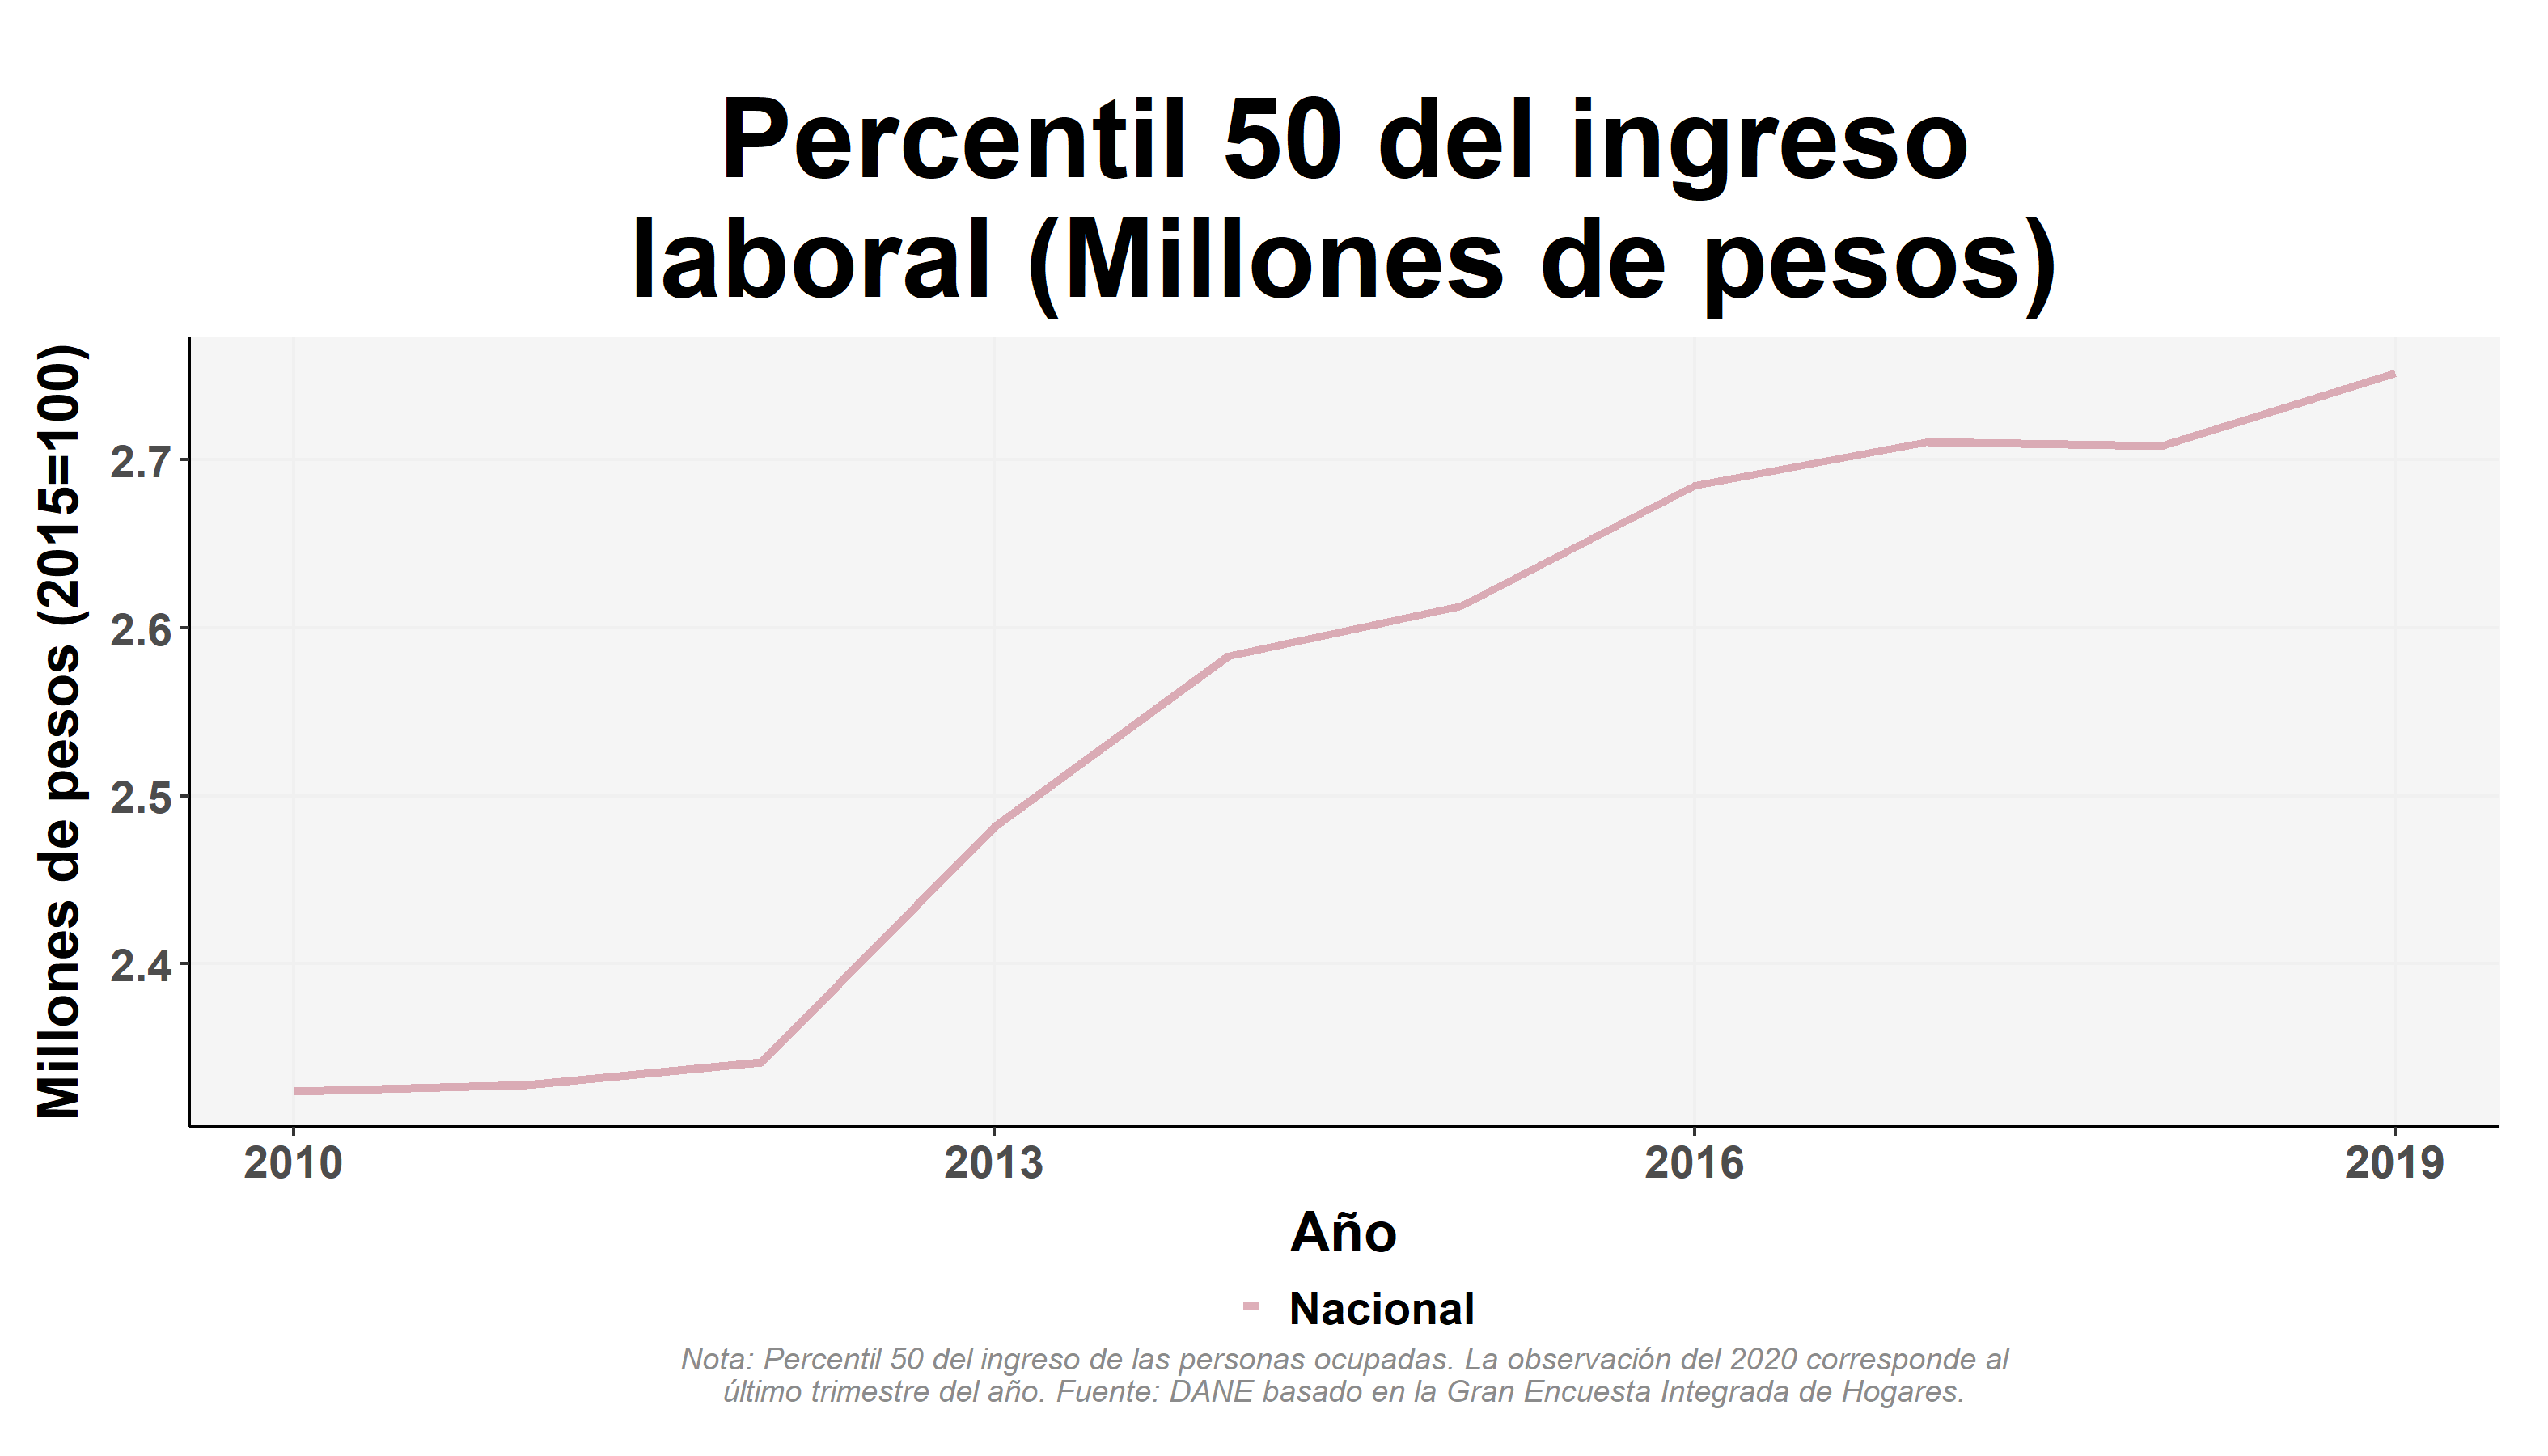
\includegraphics[width=\columnwidth]{img/var_17_trend.png}
            \end{imagecolumn}
            \begin{textcolumn}
                \begin{itemize}
                    \item El ingreso medio ha aumentado en los últimos años
                \end{itemize}
            \end{textcolumn}

    \printcolumns
    \end{slide}

    %%% Pctil 25 por genero
    \begin{slide}{3} 
            \begin{imagecolumn}
                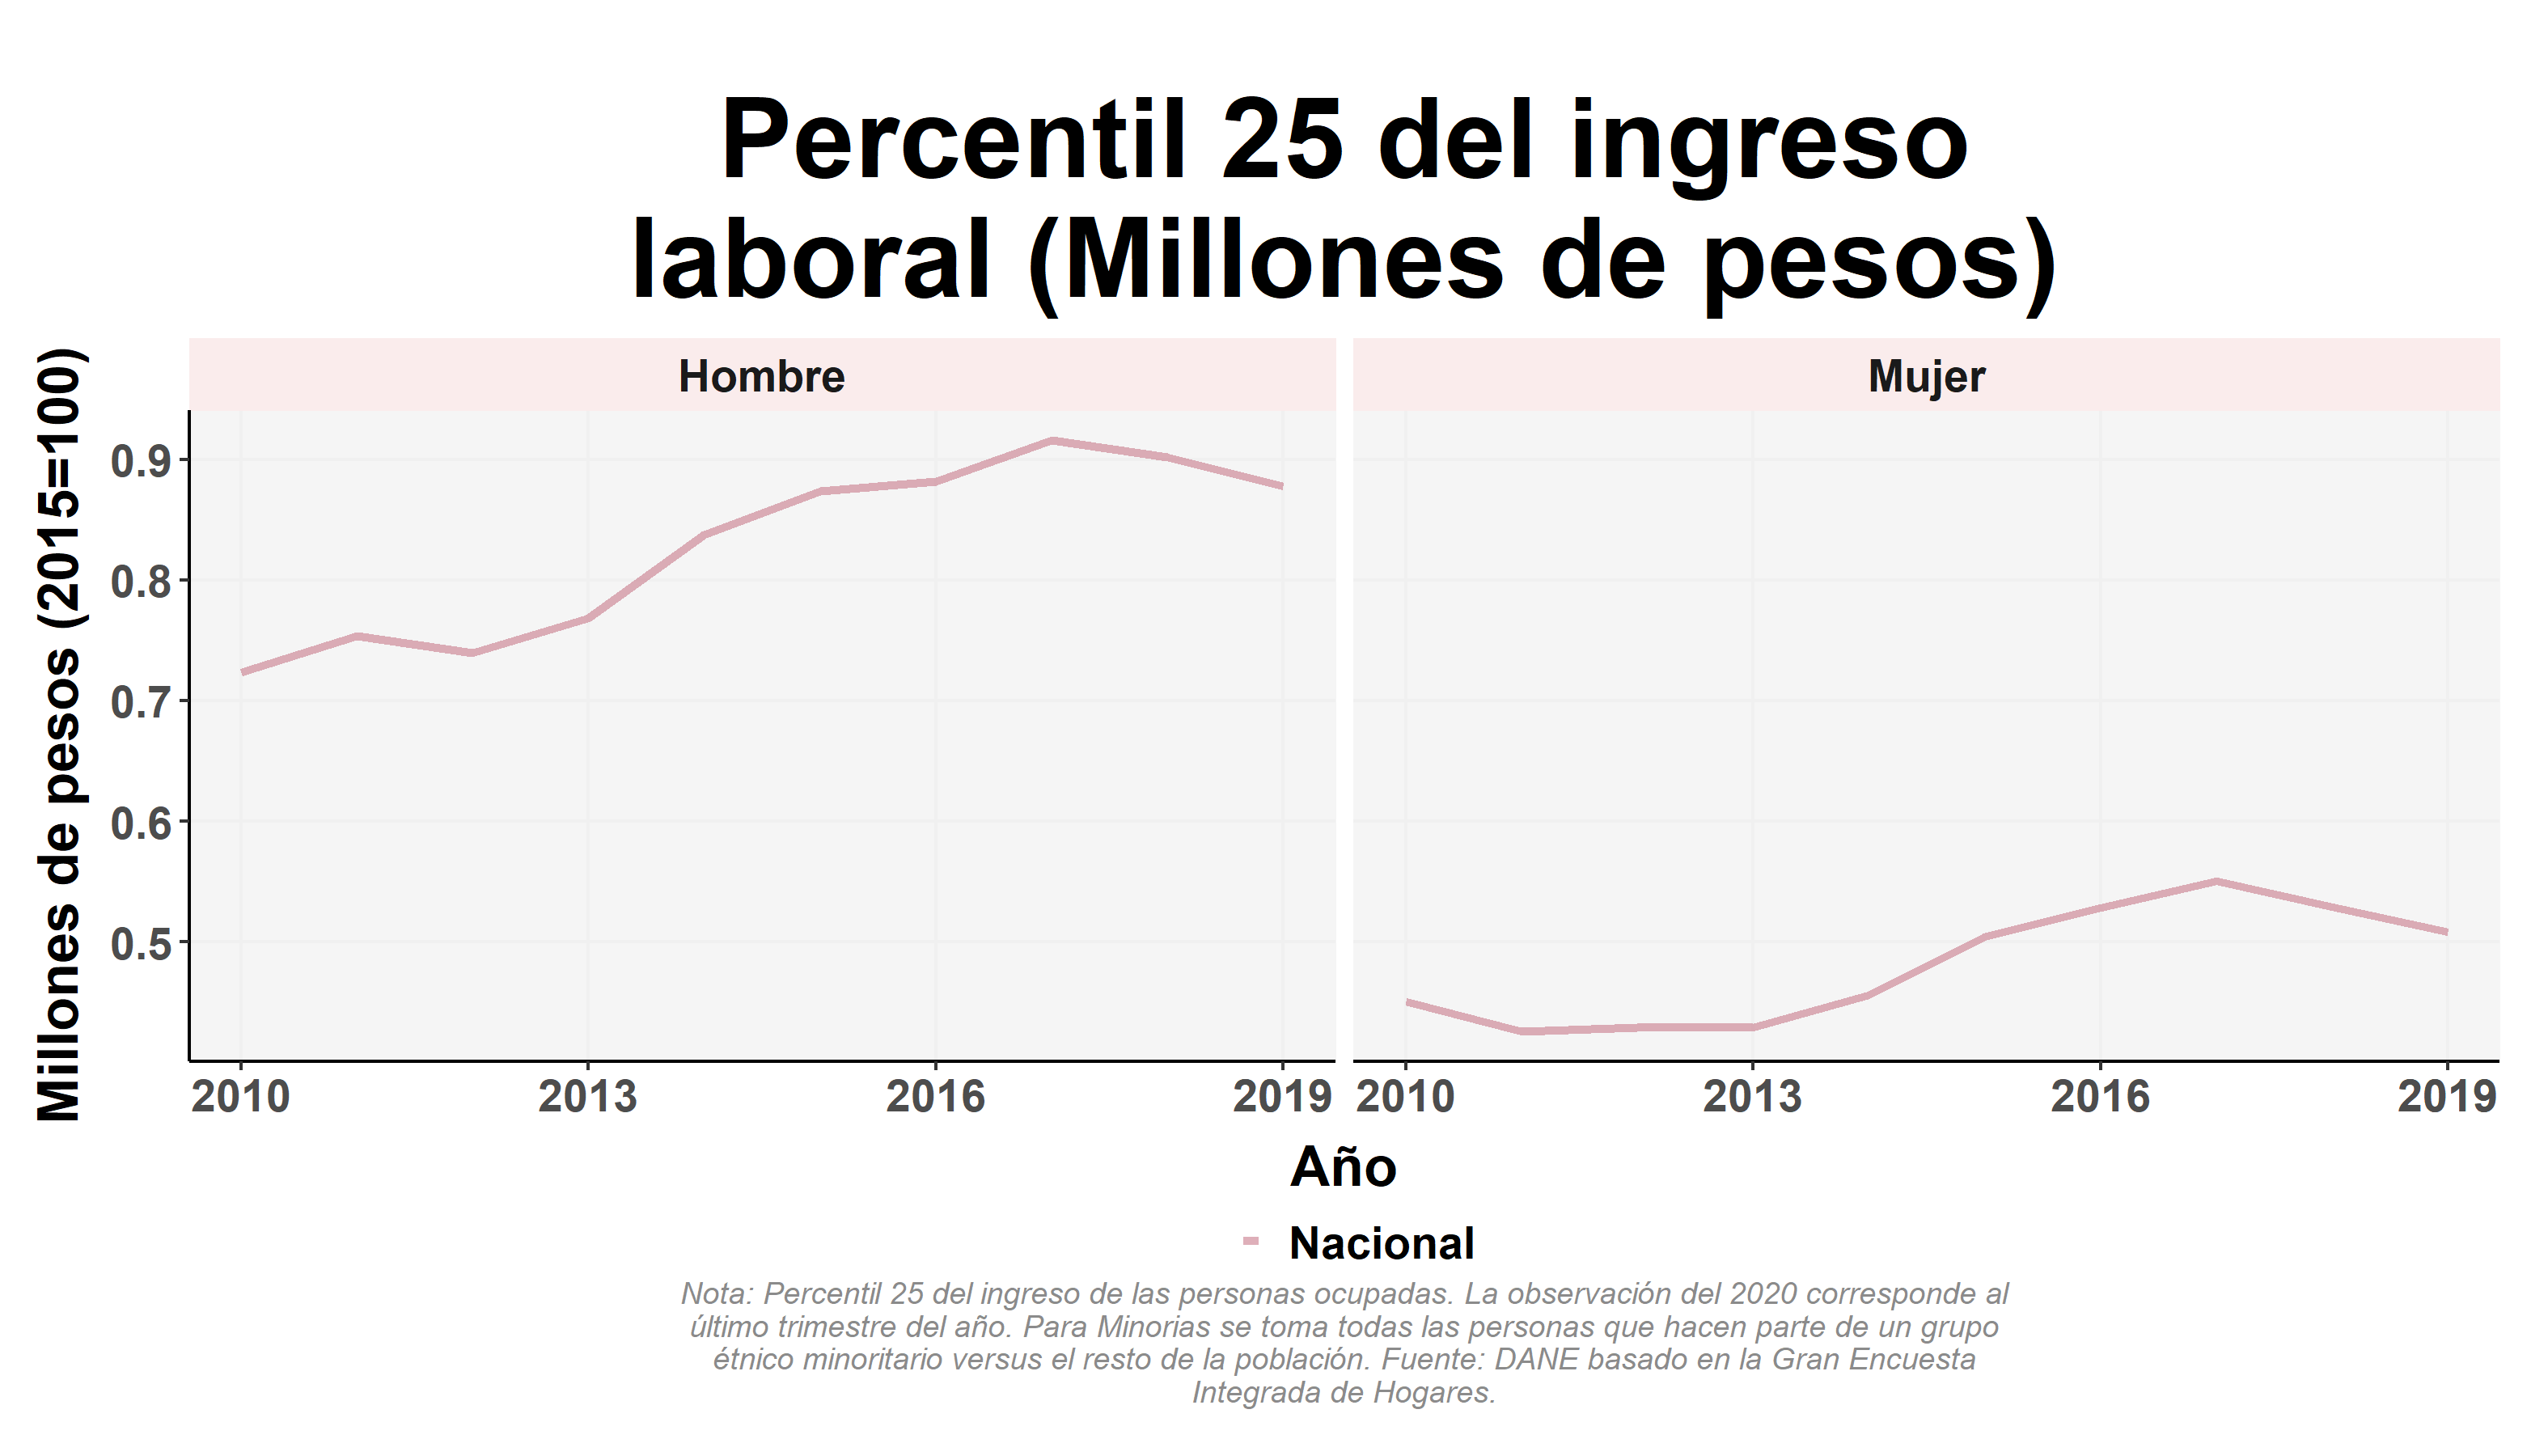
\includegraphics[width=\columnwidth]{img/var_4_trend.png}
            \end{imagecolumn}
            \begin{textcolumn}
                \begin{itemize}
                    \item Pero hay una brecha de género enorme, especialmente en los percentiles más bajos de ingreso.
                    \item Ésta brecha ha sido persistente.
                \end{itemize}
            \end{textcolumn}

    \printcolumns
    \end{slide}

    
    %%% ----------------------------
    %%% Pobreza--
    %%% ----------------------------
    \subsection{Pobreza}
    
        %%%-- No monetaria
    \begin{slide}{4} 
                      \begin{imagecolumn}
                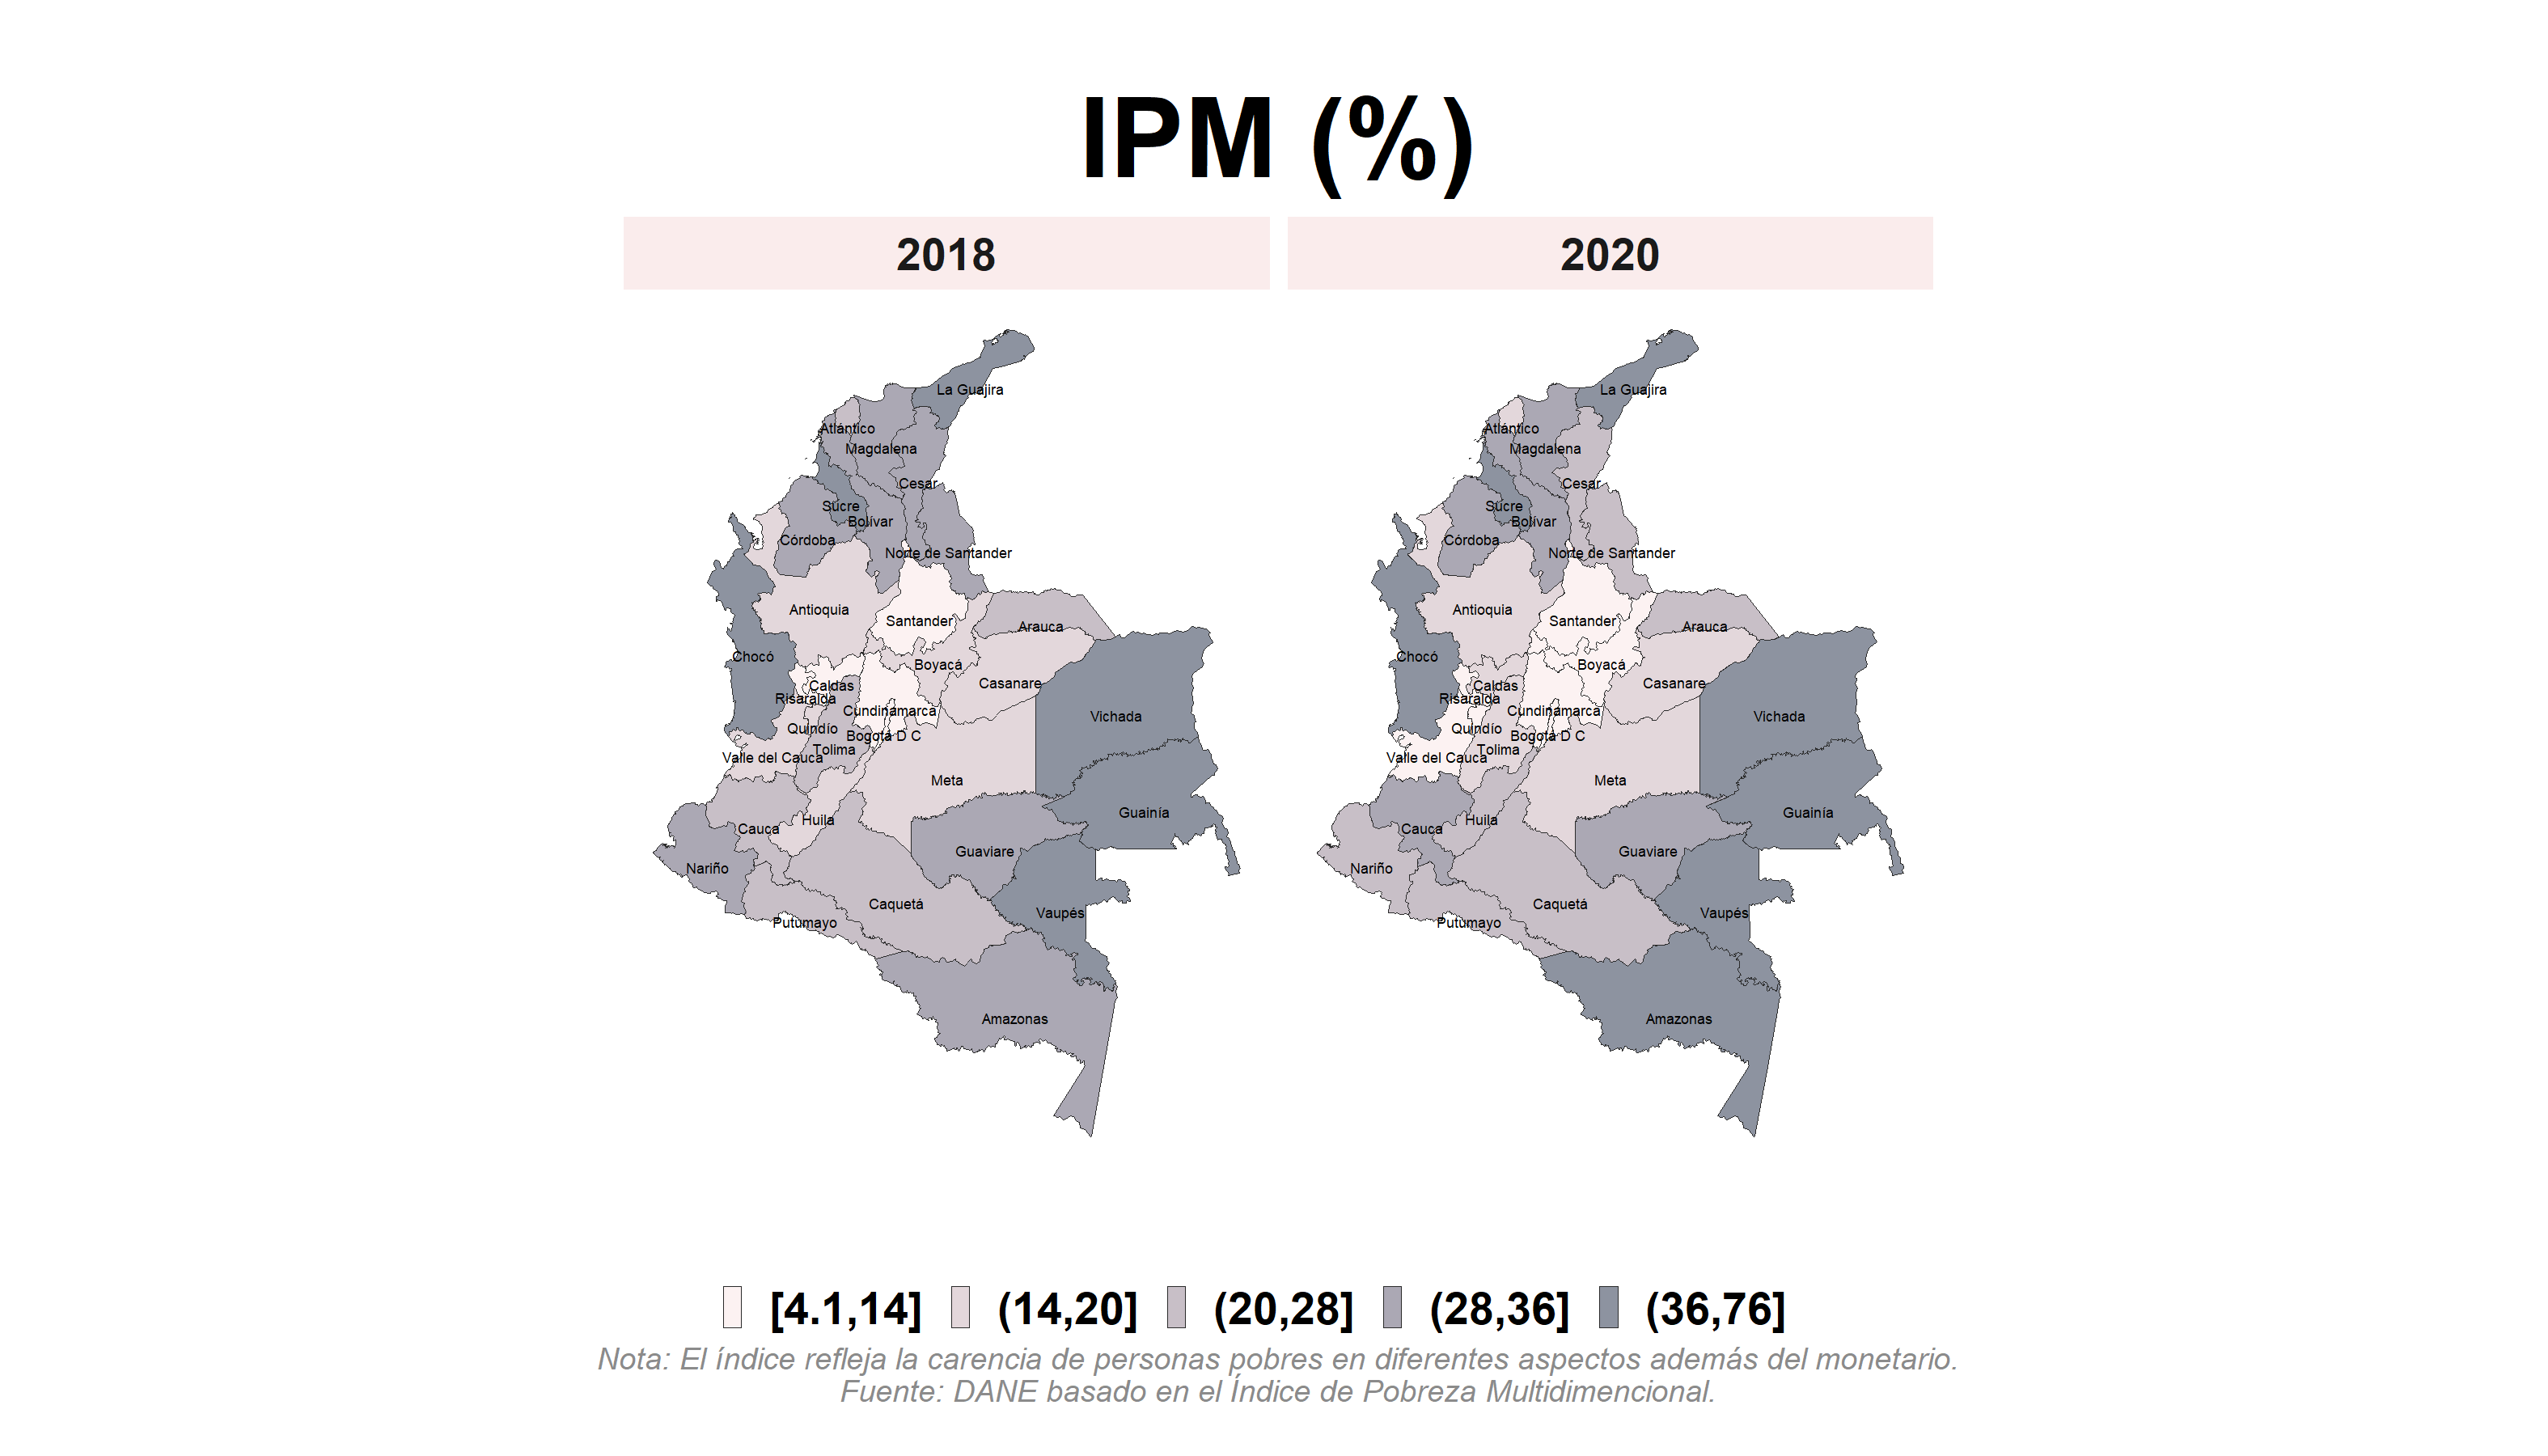
\includegraphics[width=\columnwidth]{img/var_268_map.png}
            \end{imagecolumn}
            \begin{textcolumn}
                \begin{itemize}
                    \item A nivel nacional, existe una tendencia a la baja en la pobreza no monetaria
                    \item No obstante, las brechas territoriales son grandes y persisten.
                \end{itemize}
            \end{textcolumn}

    \printcolumns
    \end{slide}
     
    %%% Monetaria
    \begin{slide}{4} 
            \begin{imagecolumn}
                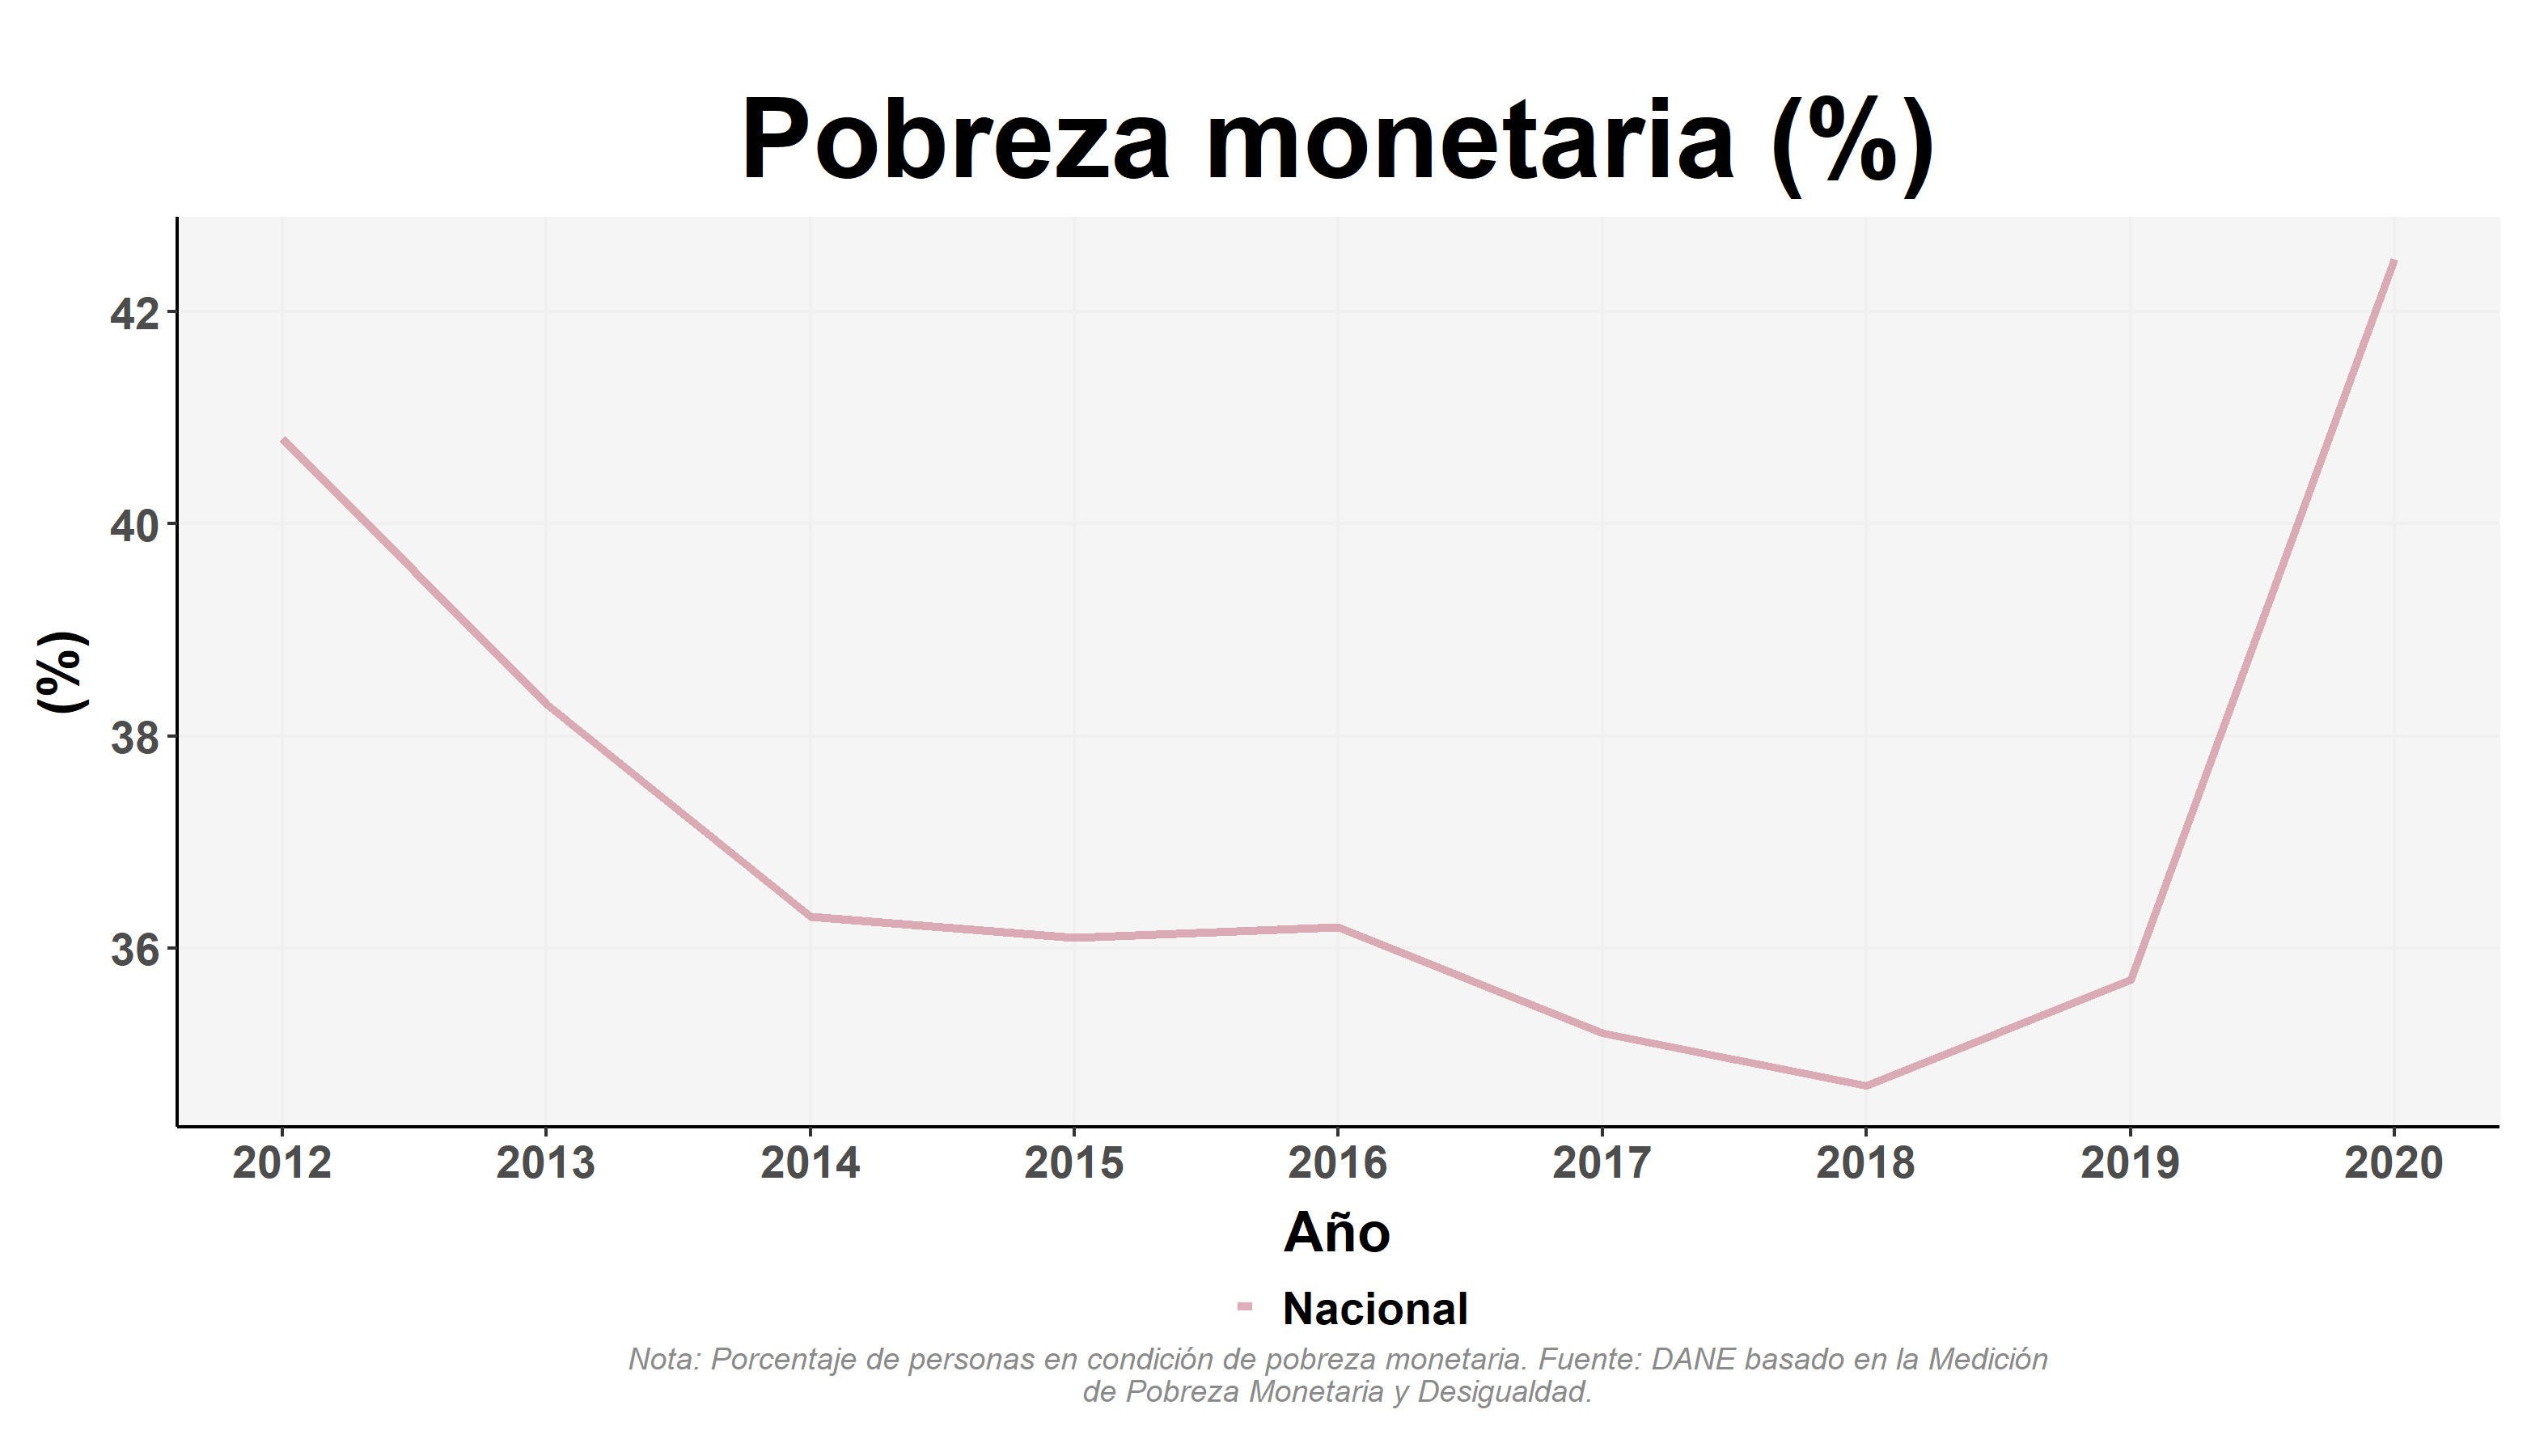
\includegraphics[width=\columnwidth]{img/var_263_trend.png}
            \end{imagecolumn}
            \begin{textcolumn}
                \begin{itemize}
                    \item La pobreza monetaria había estado bajando de forma sostenida hasta antes de la pandemia
                    \item Pero retrocedió a niveles aún mayores de los que se observaban 10 años atrás
                \end{itemize}
            \end{textcolumn}

    \printcolumns
    \end{slide}
    
        %%% Pobreza por zonas
    \begin{slide}{4} 
            \begin{imagecolumn}
                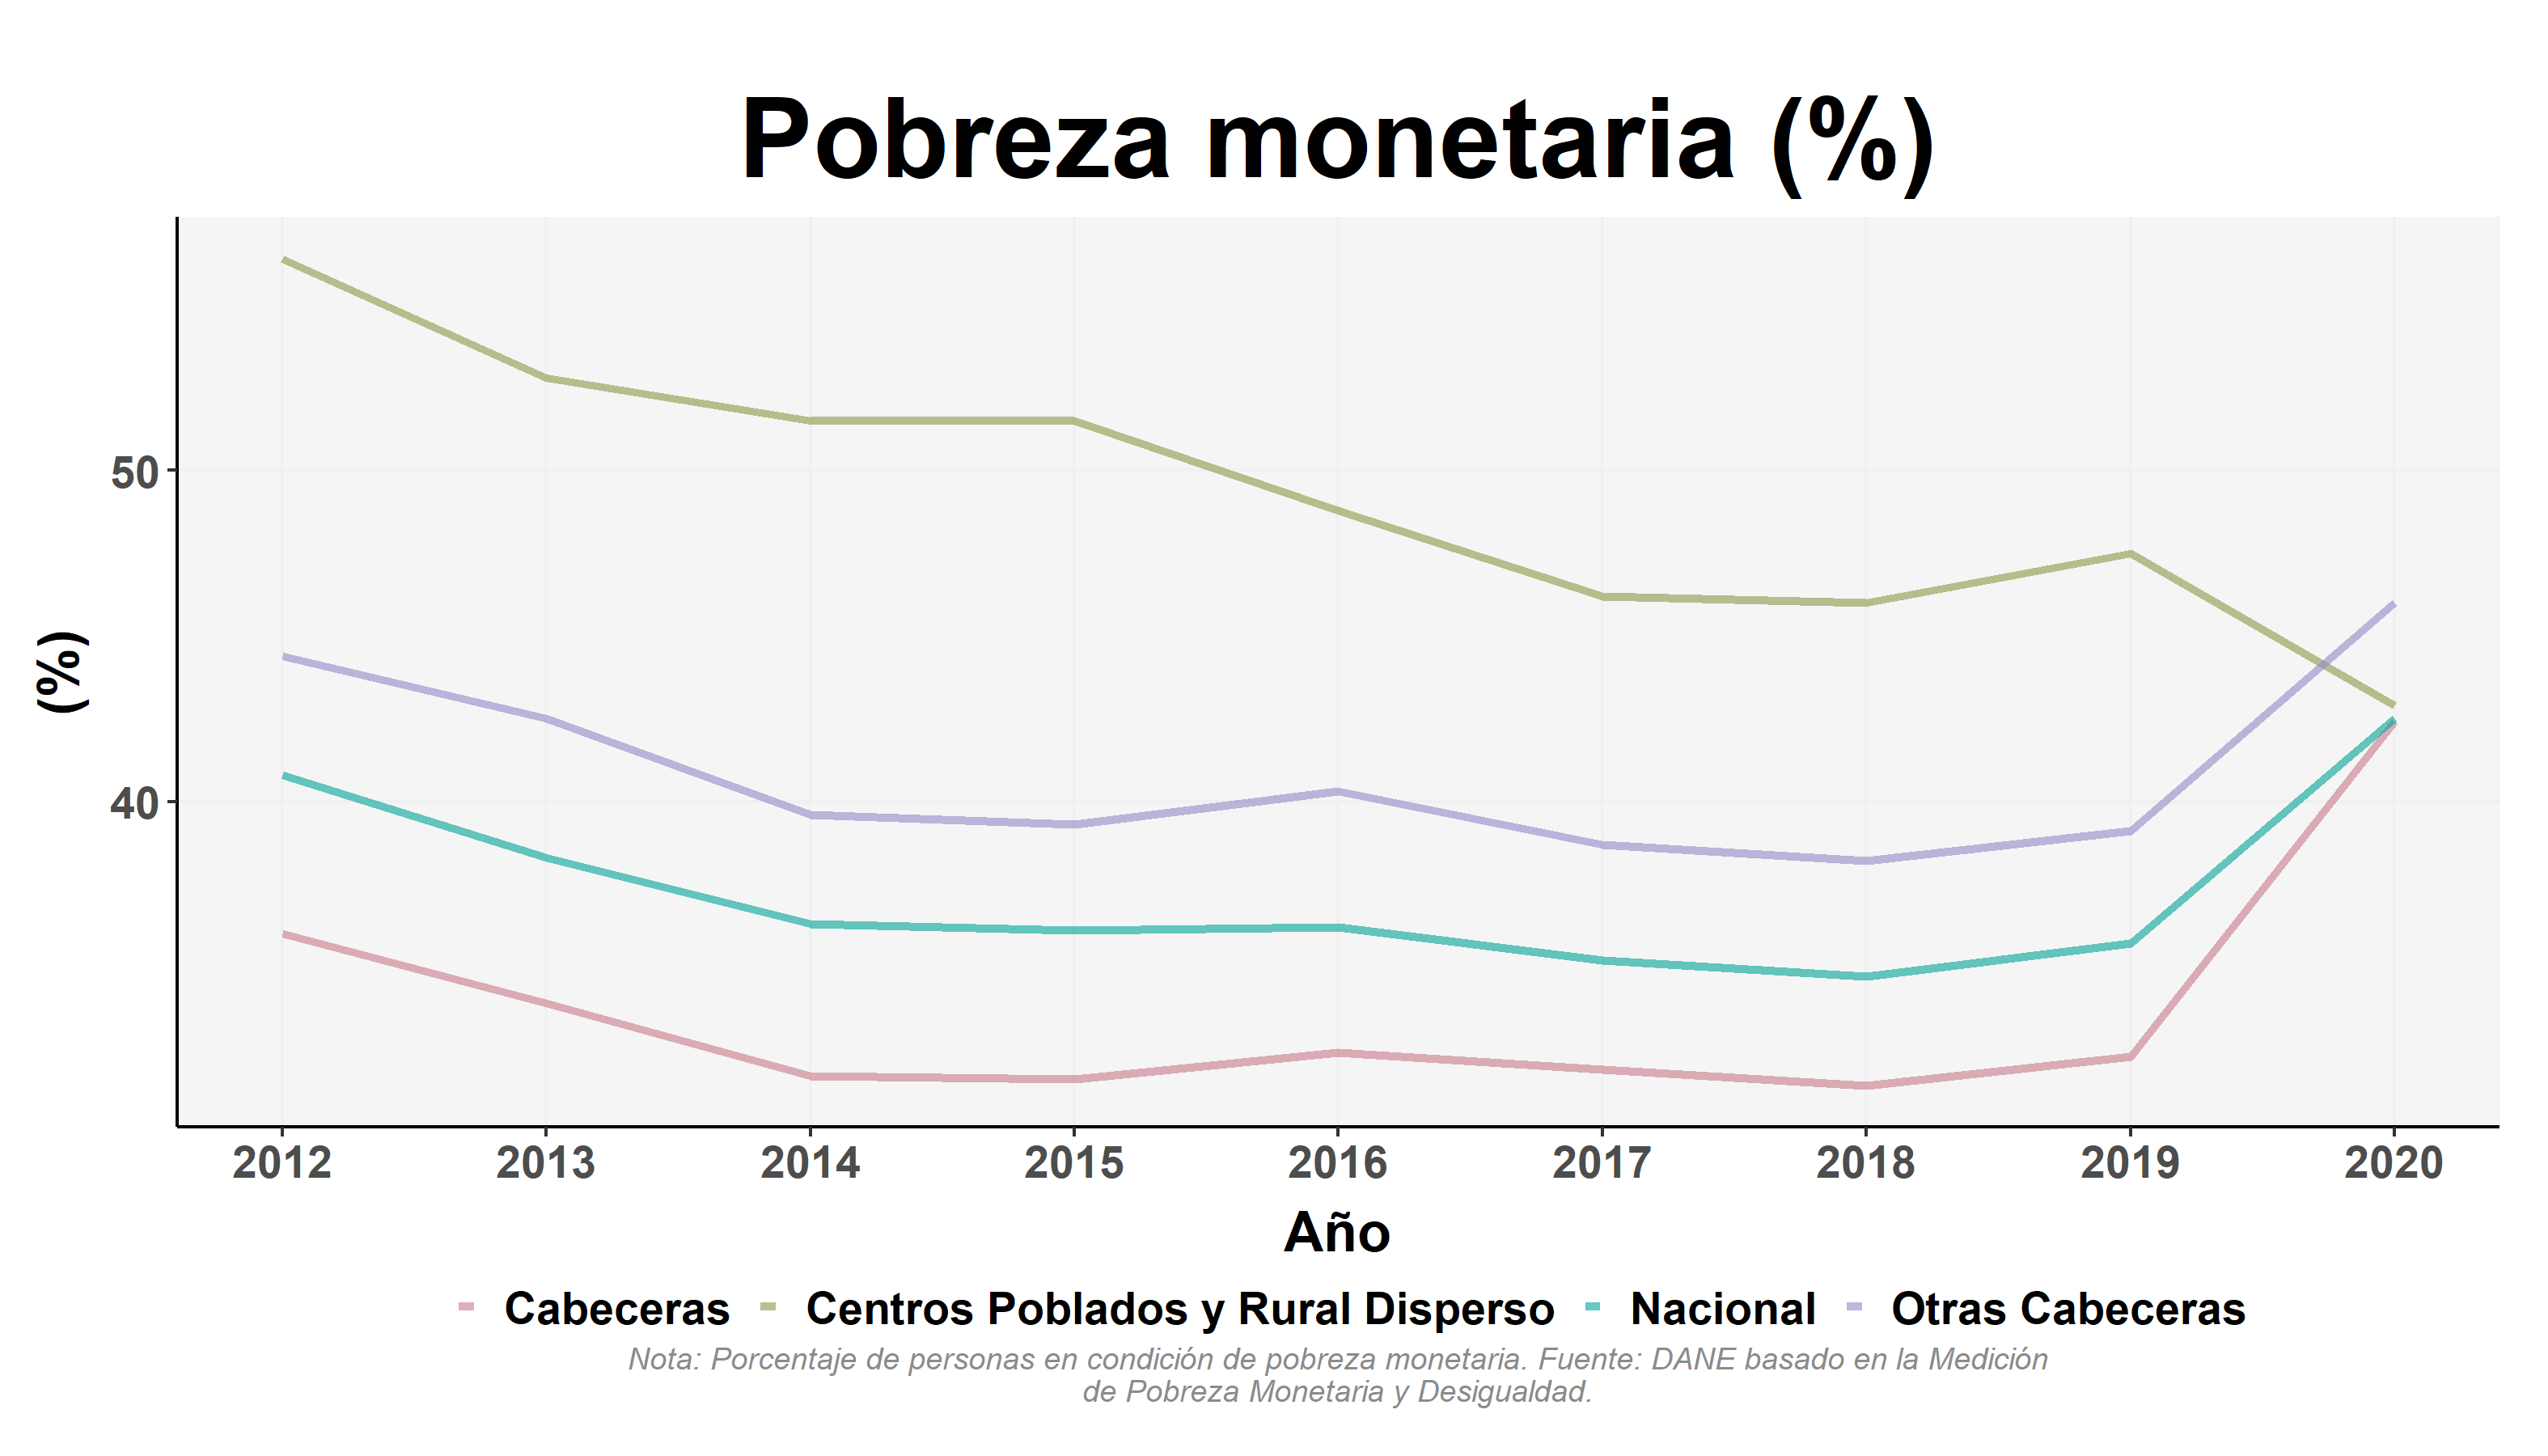
\includegraphics[width=\columnwidth]{img/var_264_trend.png}
            \end{imagecolumn}
            \begin{textcolumn}
                \begin{itemize}
                    \item La pandemia generó convergencia entre zonas urbanas y rurales, por el drástico aumento de la pobreza en las ciudades.
                \end{itemize}
            \end{textcolumn}

    \printcolumns
    \end{slide}
    
    
    %%% ----------------------------
    %%% Desigualdad--
    %%% ----------------------------
    \subsection{Desigualdad}
 
     %%% Gini zonas
    \begin{slide}{5} 
            \begin{imagecolumn}
                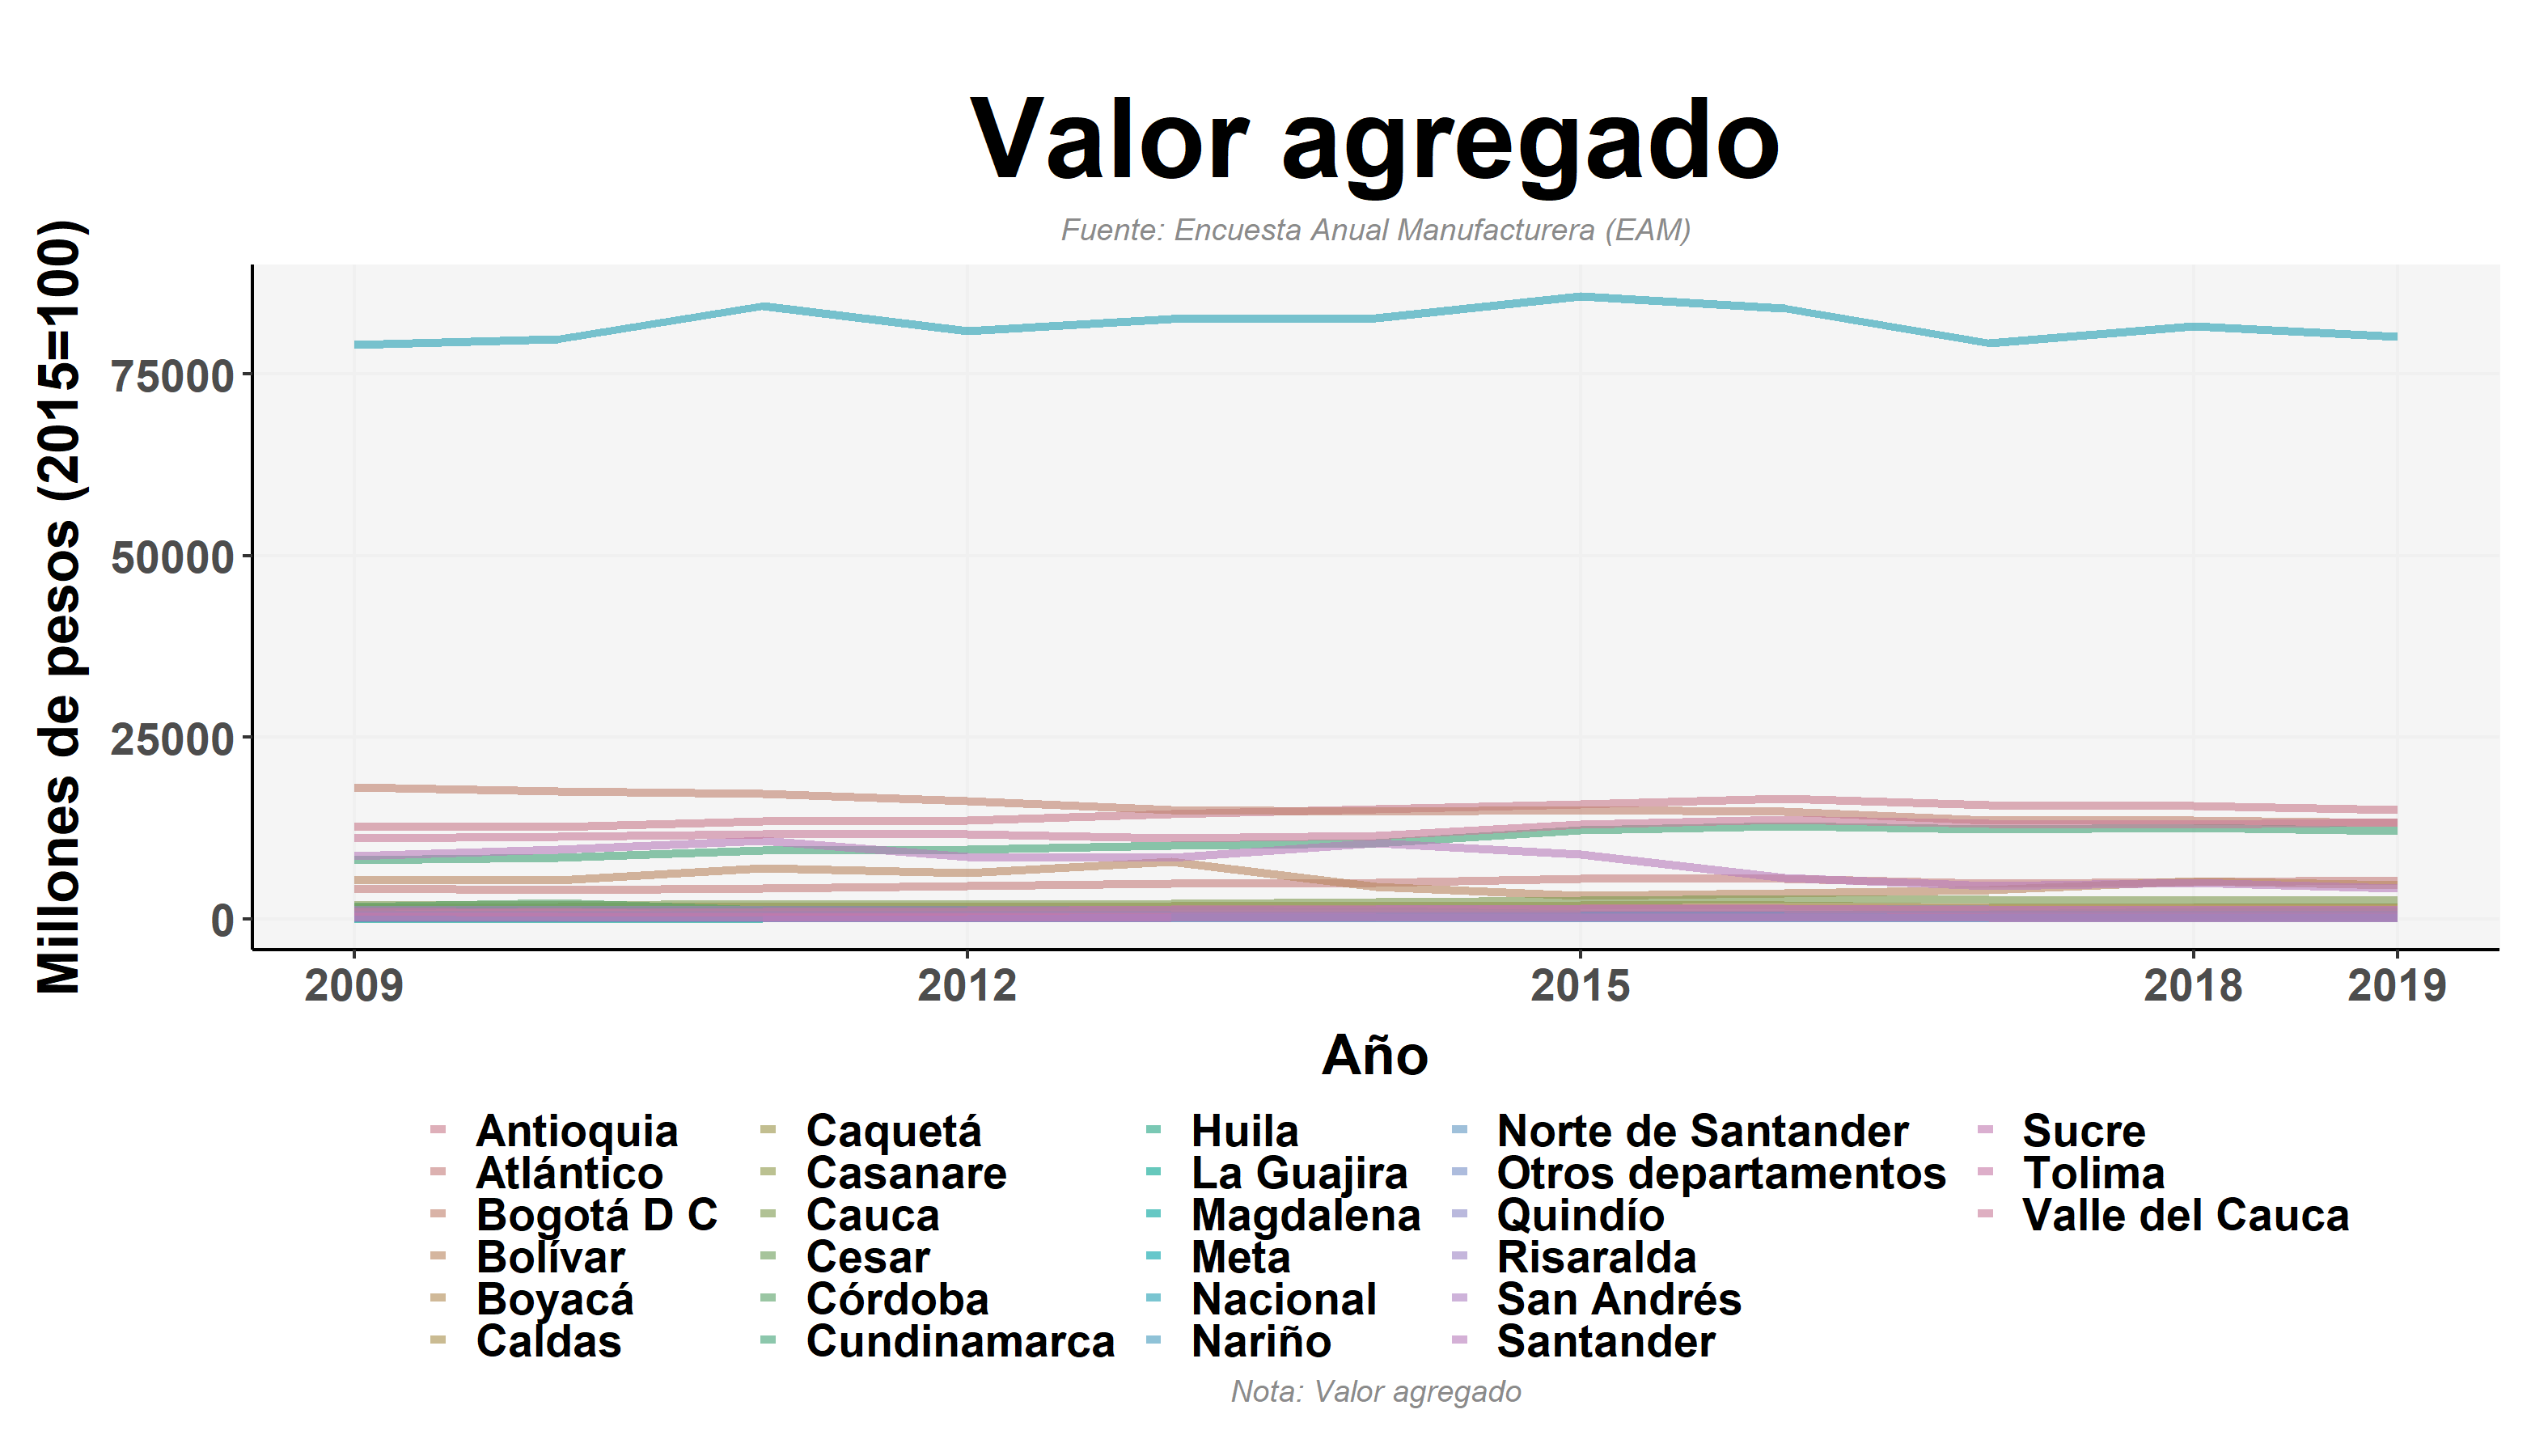
\includegraphics[width=\columnwidth]{img/var_256_trend.png}
            \end{imagecolumn}
            \begin{textcolumn}
                \begin{itemize}
                    \item Hasta 2017 la desigualdad venia disminuyendo en todas las zonas, pero la pandemia devolvió a los territorios a los niveles de desigualdad de hace 10 años.
                \end{itemize}
            \end{textcolumn}

    \printcolumns
    \end{slide}
    
        %%%-- Gini departamentos 
    \begin{slide}{5} 
                      \begin{imagecolumn}
                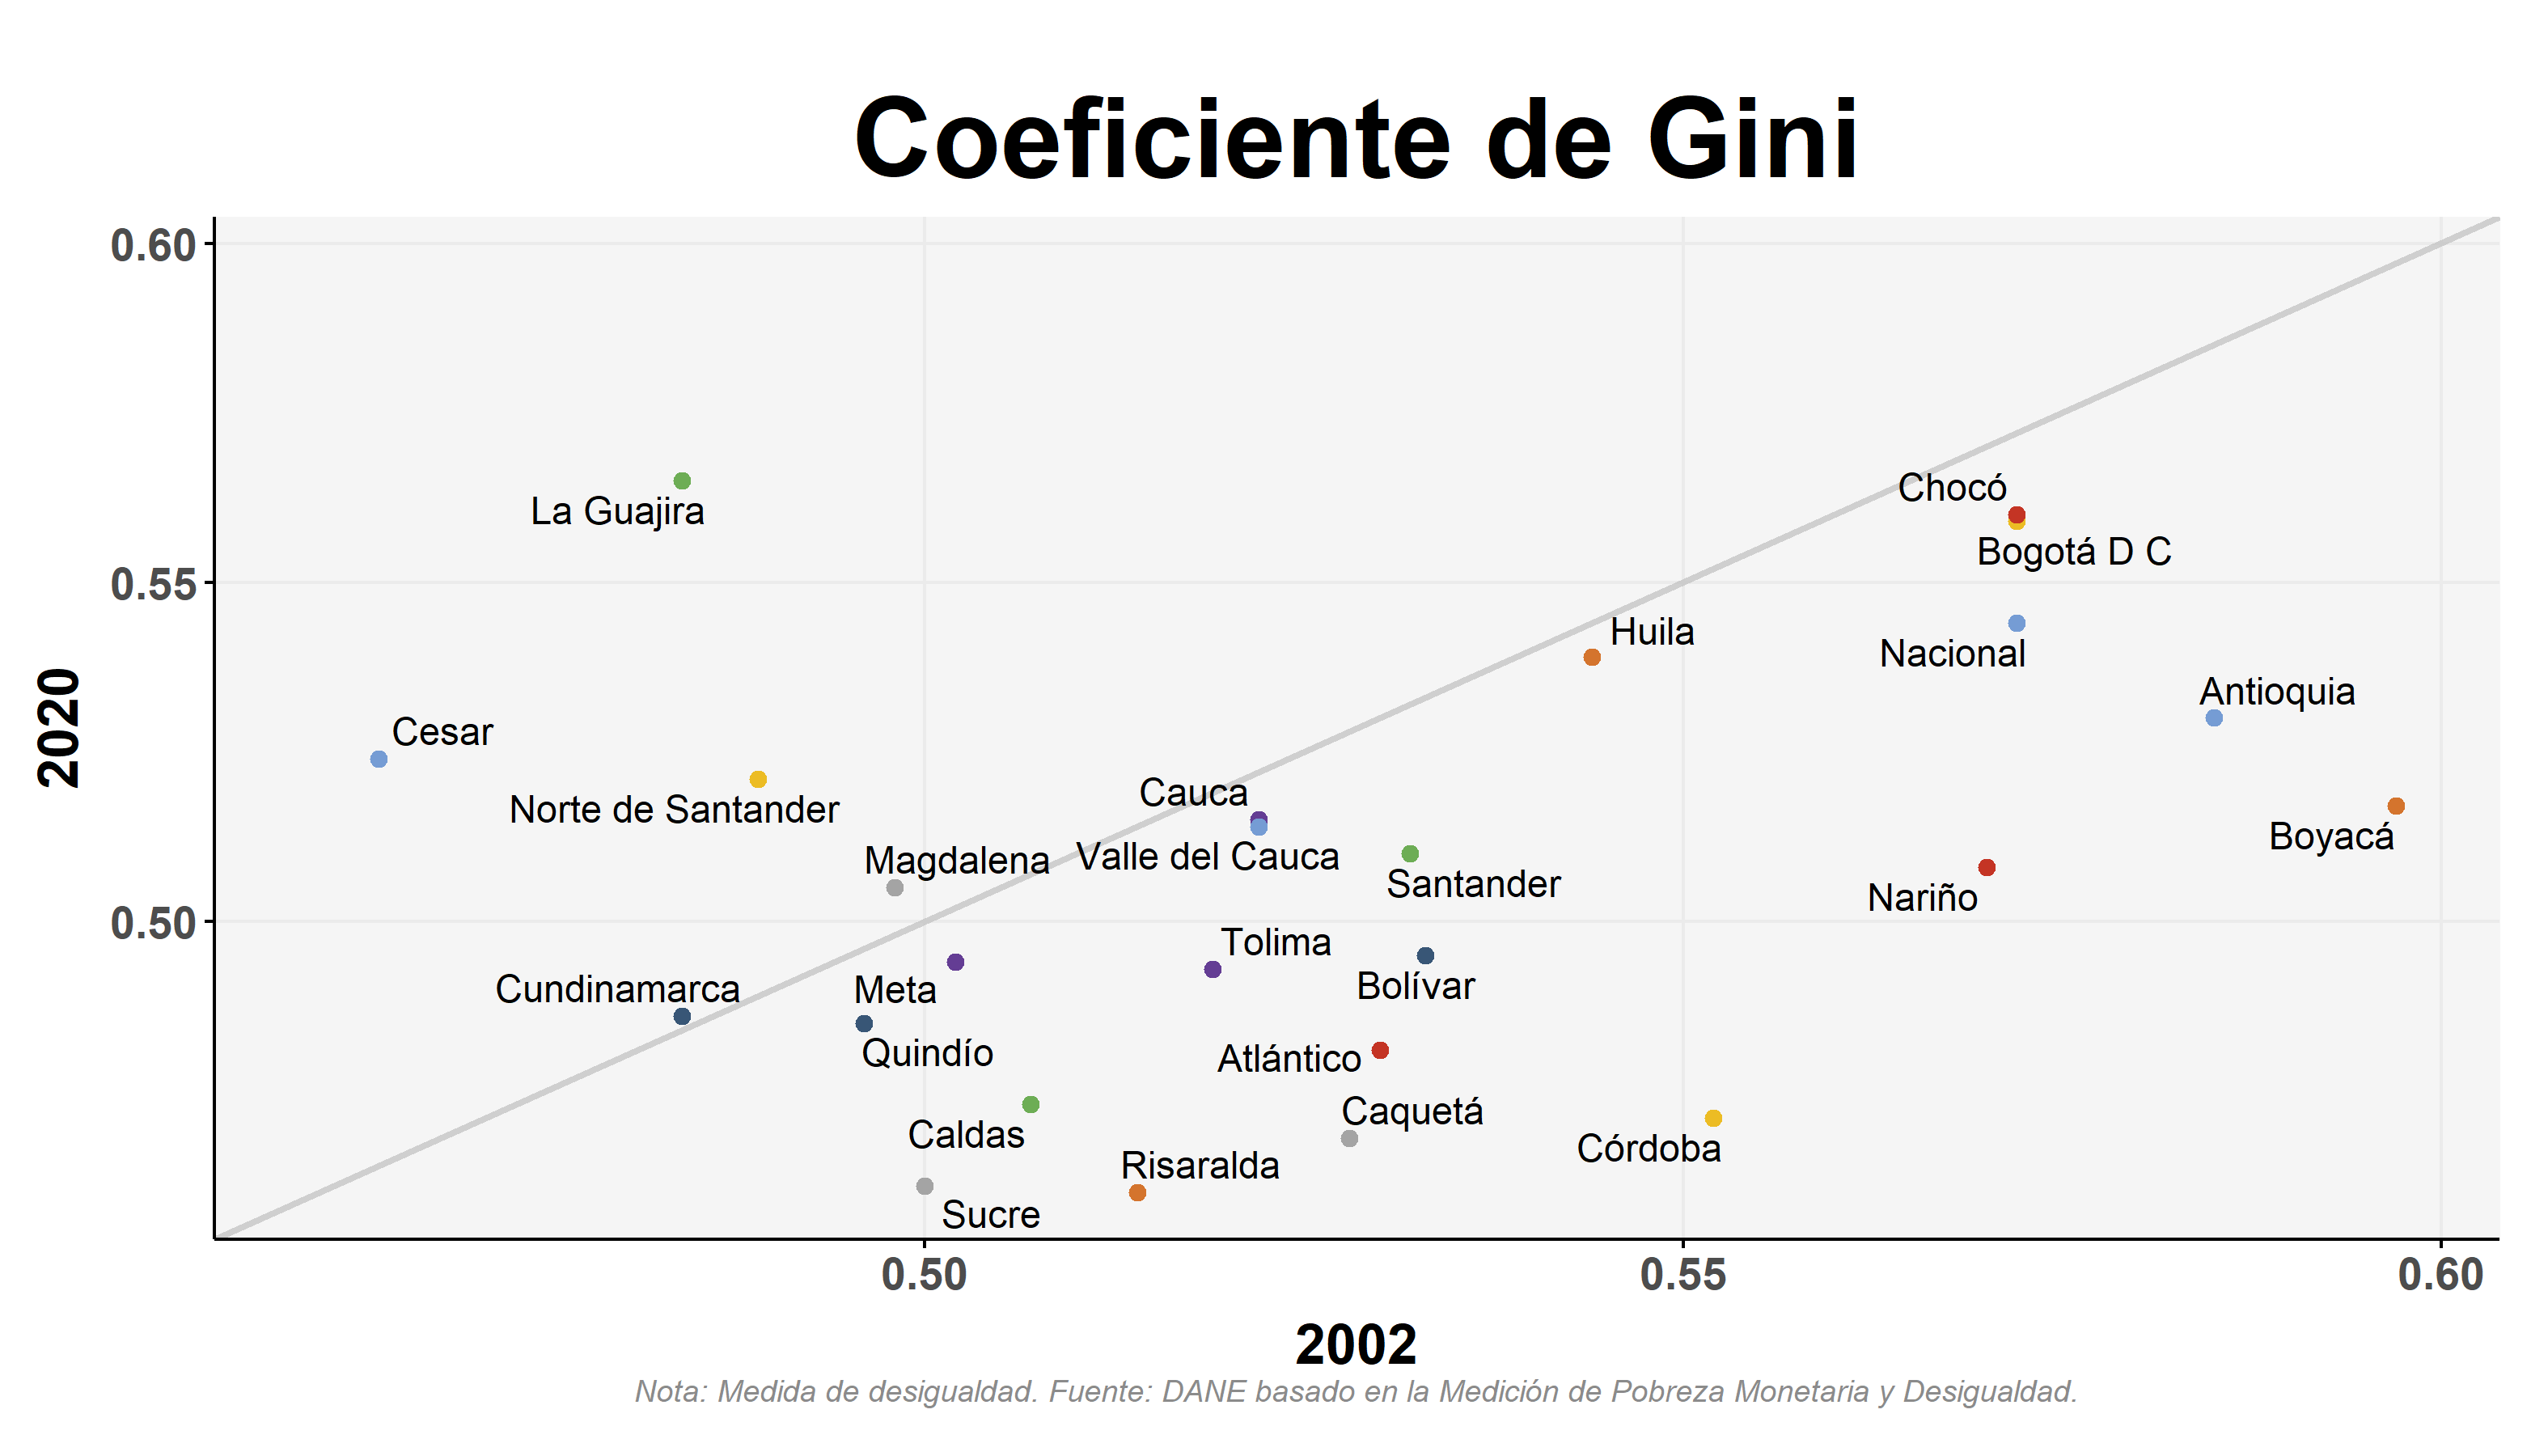
\includegraphics[width=\columnwidth]{img/var_254_scatter_time.png}
            \end{imagecolumn}
            \begin{textcolumn}
                \begin{itemize}
                    \item Aún así, comparado con 2002 la desigualdad ha disminuido en muchos territorios
                    \item Pero algunos departamentos como Chocó y el Huila persisten en sus niveles de desigualdad de hace 20 años.
                \end{itemize}
            \end{textcolumn}

    \printcolumns
    \end{slide}
     
    

    
    %%% ----------------------------
    %%% Características del hogar
    %%% ----------------------------
    \subsection{Característica del hogar}
    
        %%%-- Hacinamiento Crítico 
    \begin{slide}{6} 
                      \begin{imagecolumn}
                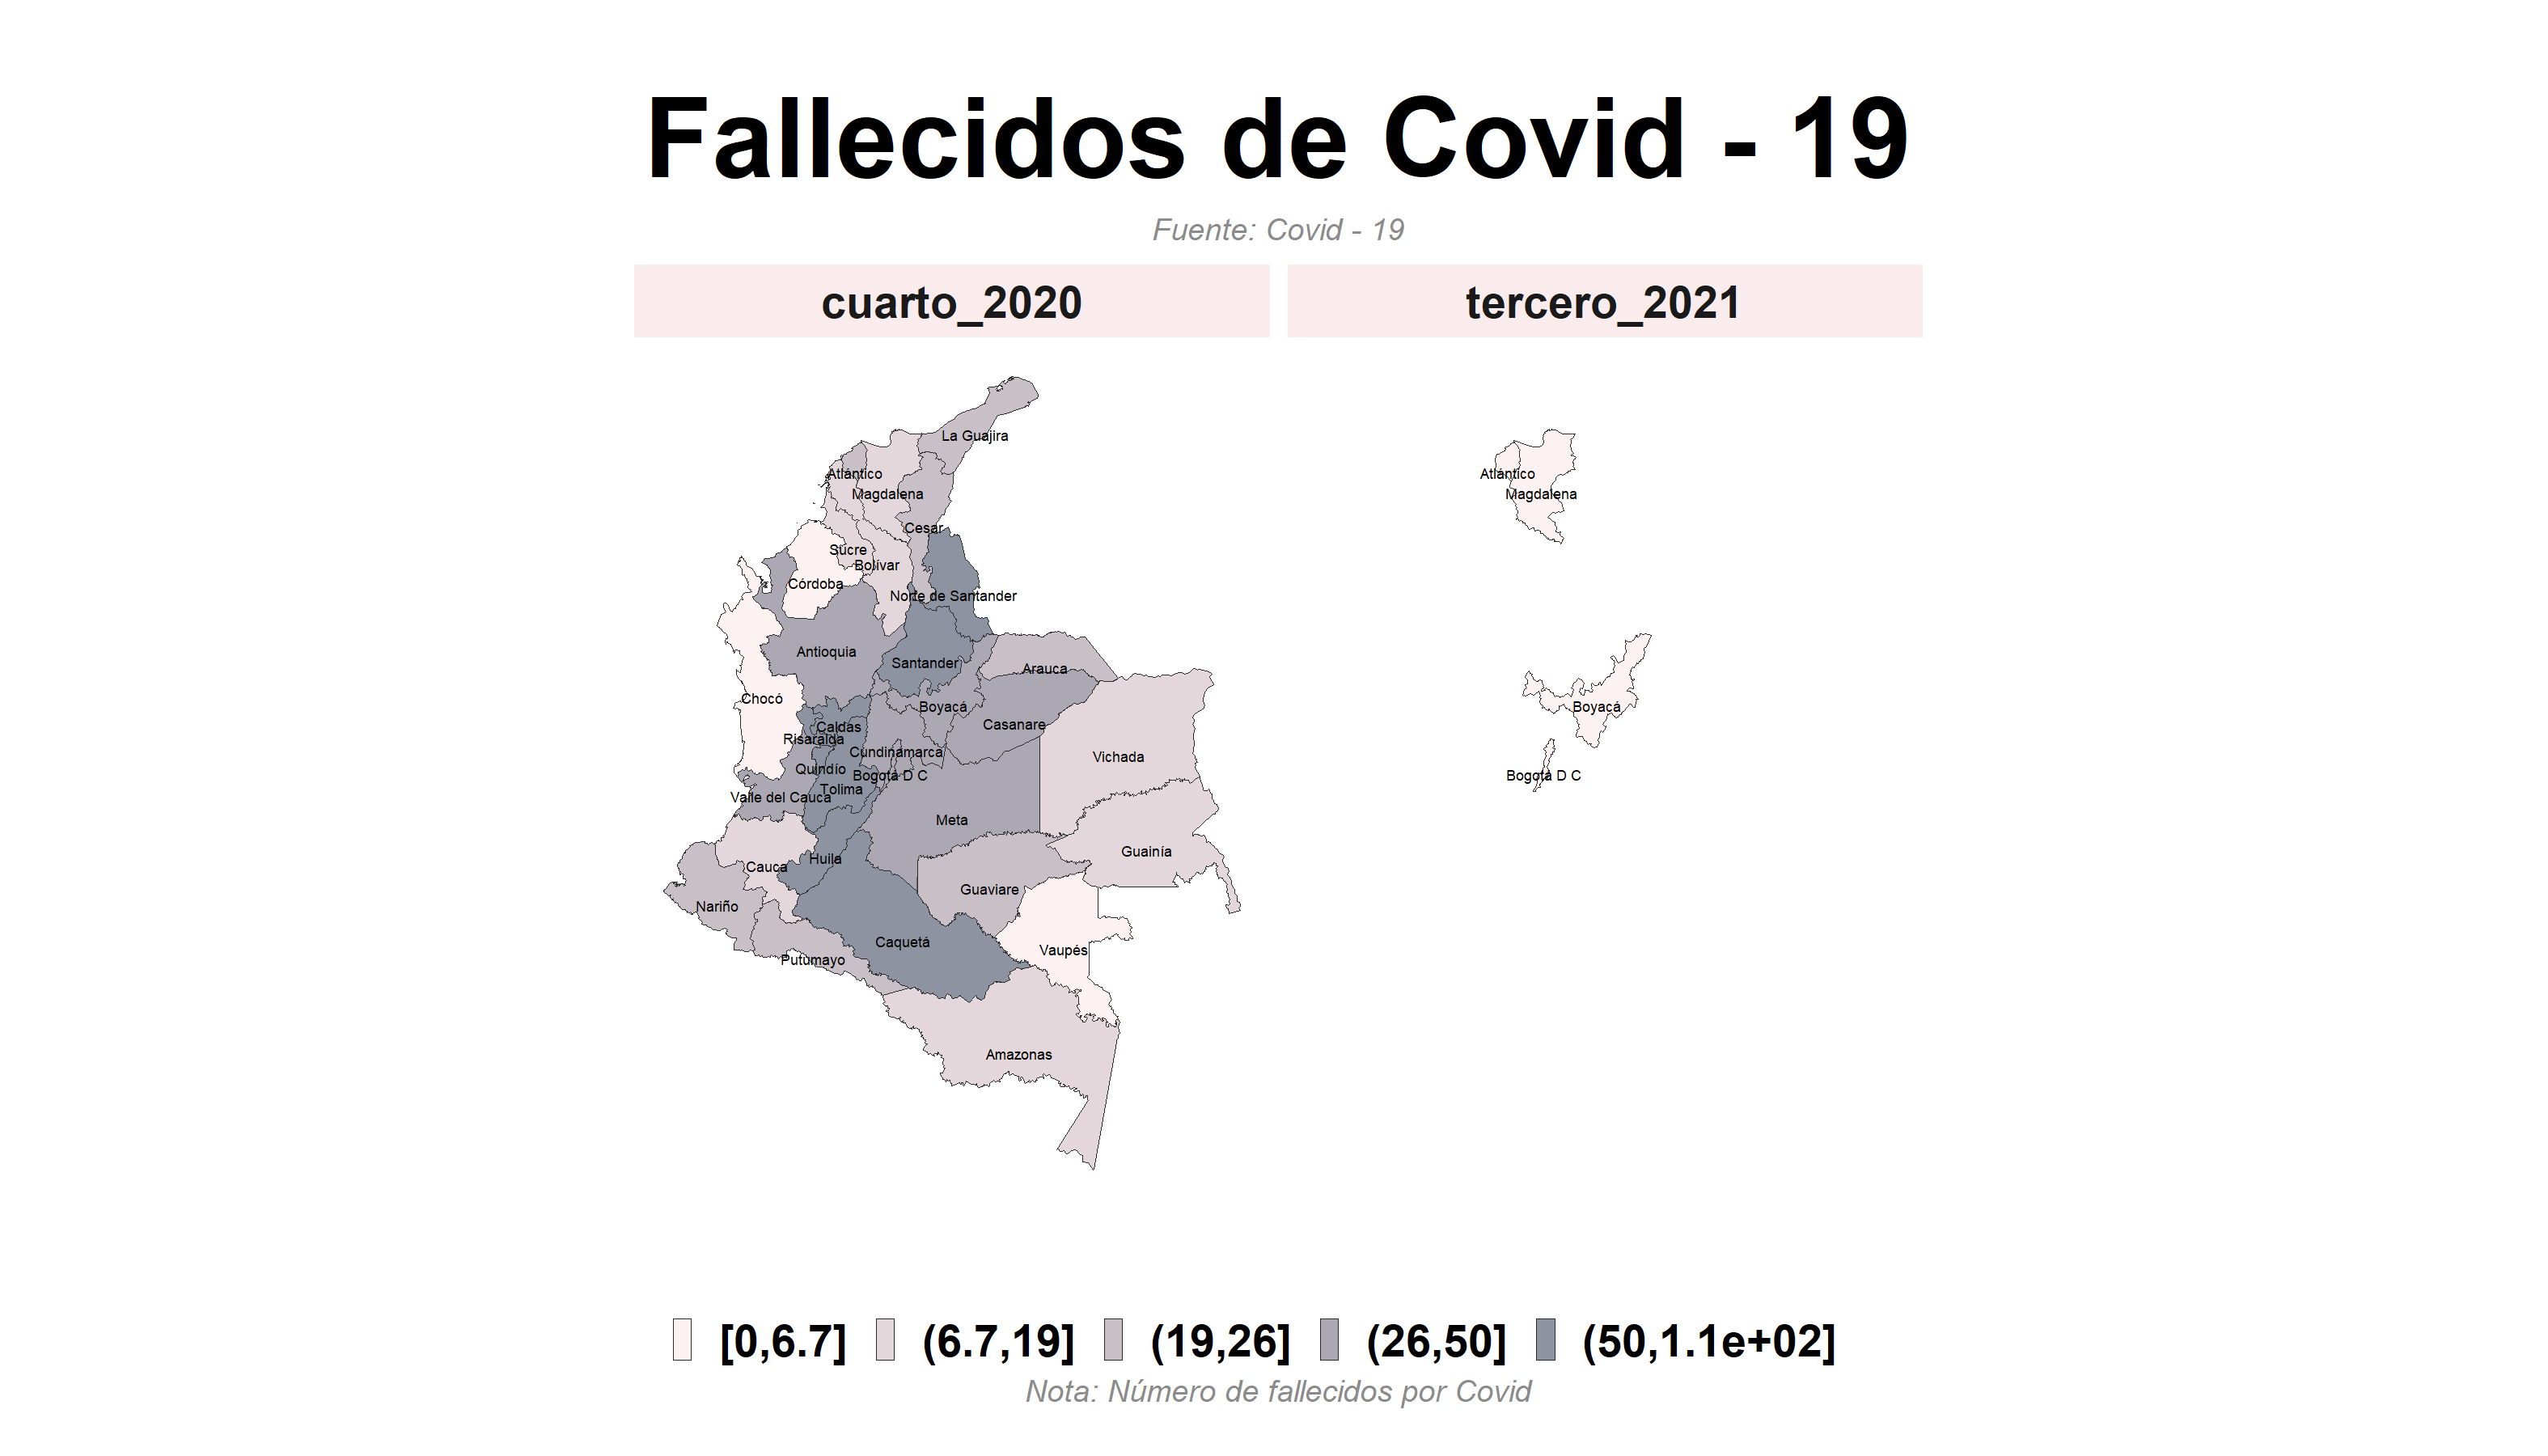
\includegraphics[width=\columnwidth]{img/var_265_map.png}
            \end{imagecolumn}
            \begin{textcolumn}
                \begin{itemize}
                    \item Existe una alta variación en el hacinamiento crítico entre regiones 
                    \item Esto puede estar asociado a las estructuras étnicas en algunos departamentos
                \end{itemize}
            \end{textcolumn}

    \printcolumns
    \end{slide}
    
    
        
    %%% ----------------------------
    %%% Acceso a Agua Potable
    %%% ----------------------------
    \subsection{Acceso a servicios de Agua Potable}
    
        %%%-- Highlights 
    \begin{slide}{7} 
                      \begin{imagecolumn}
                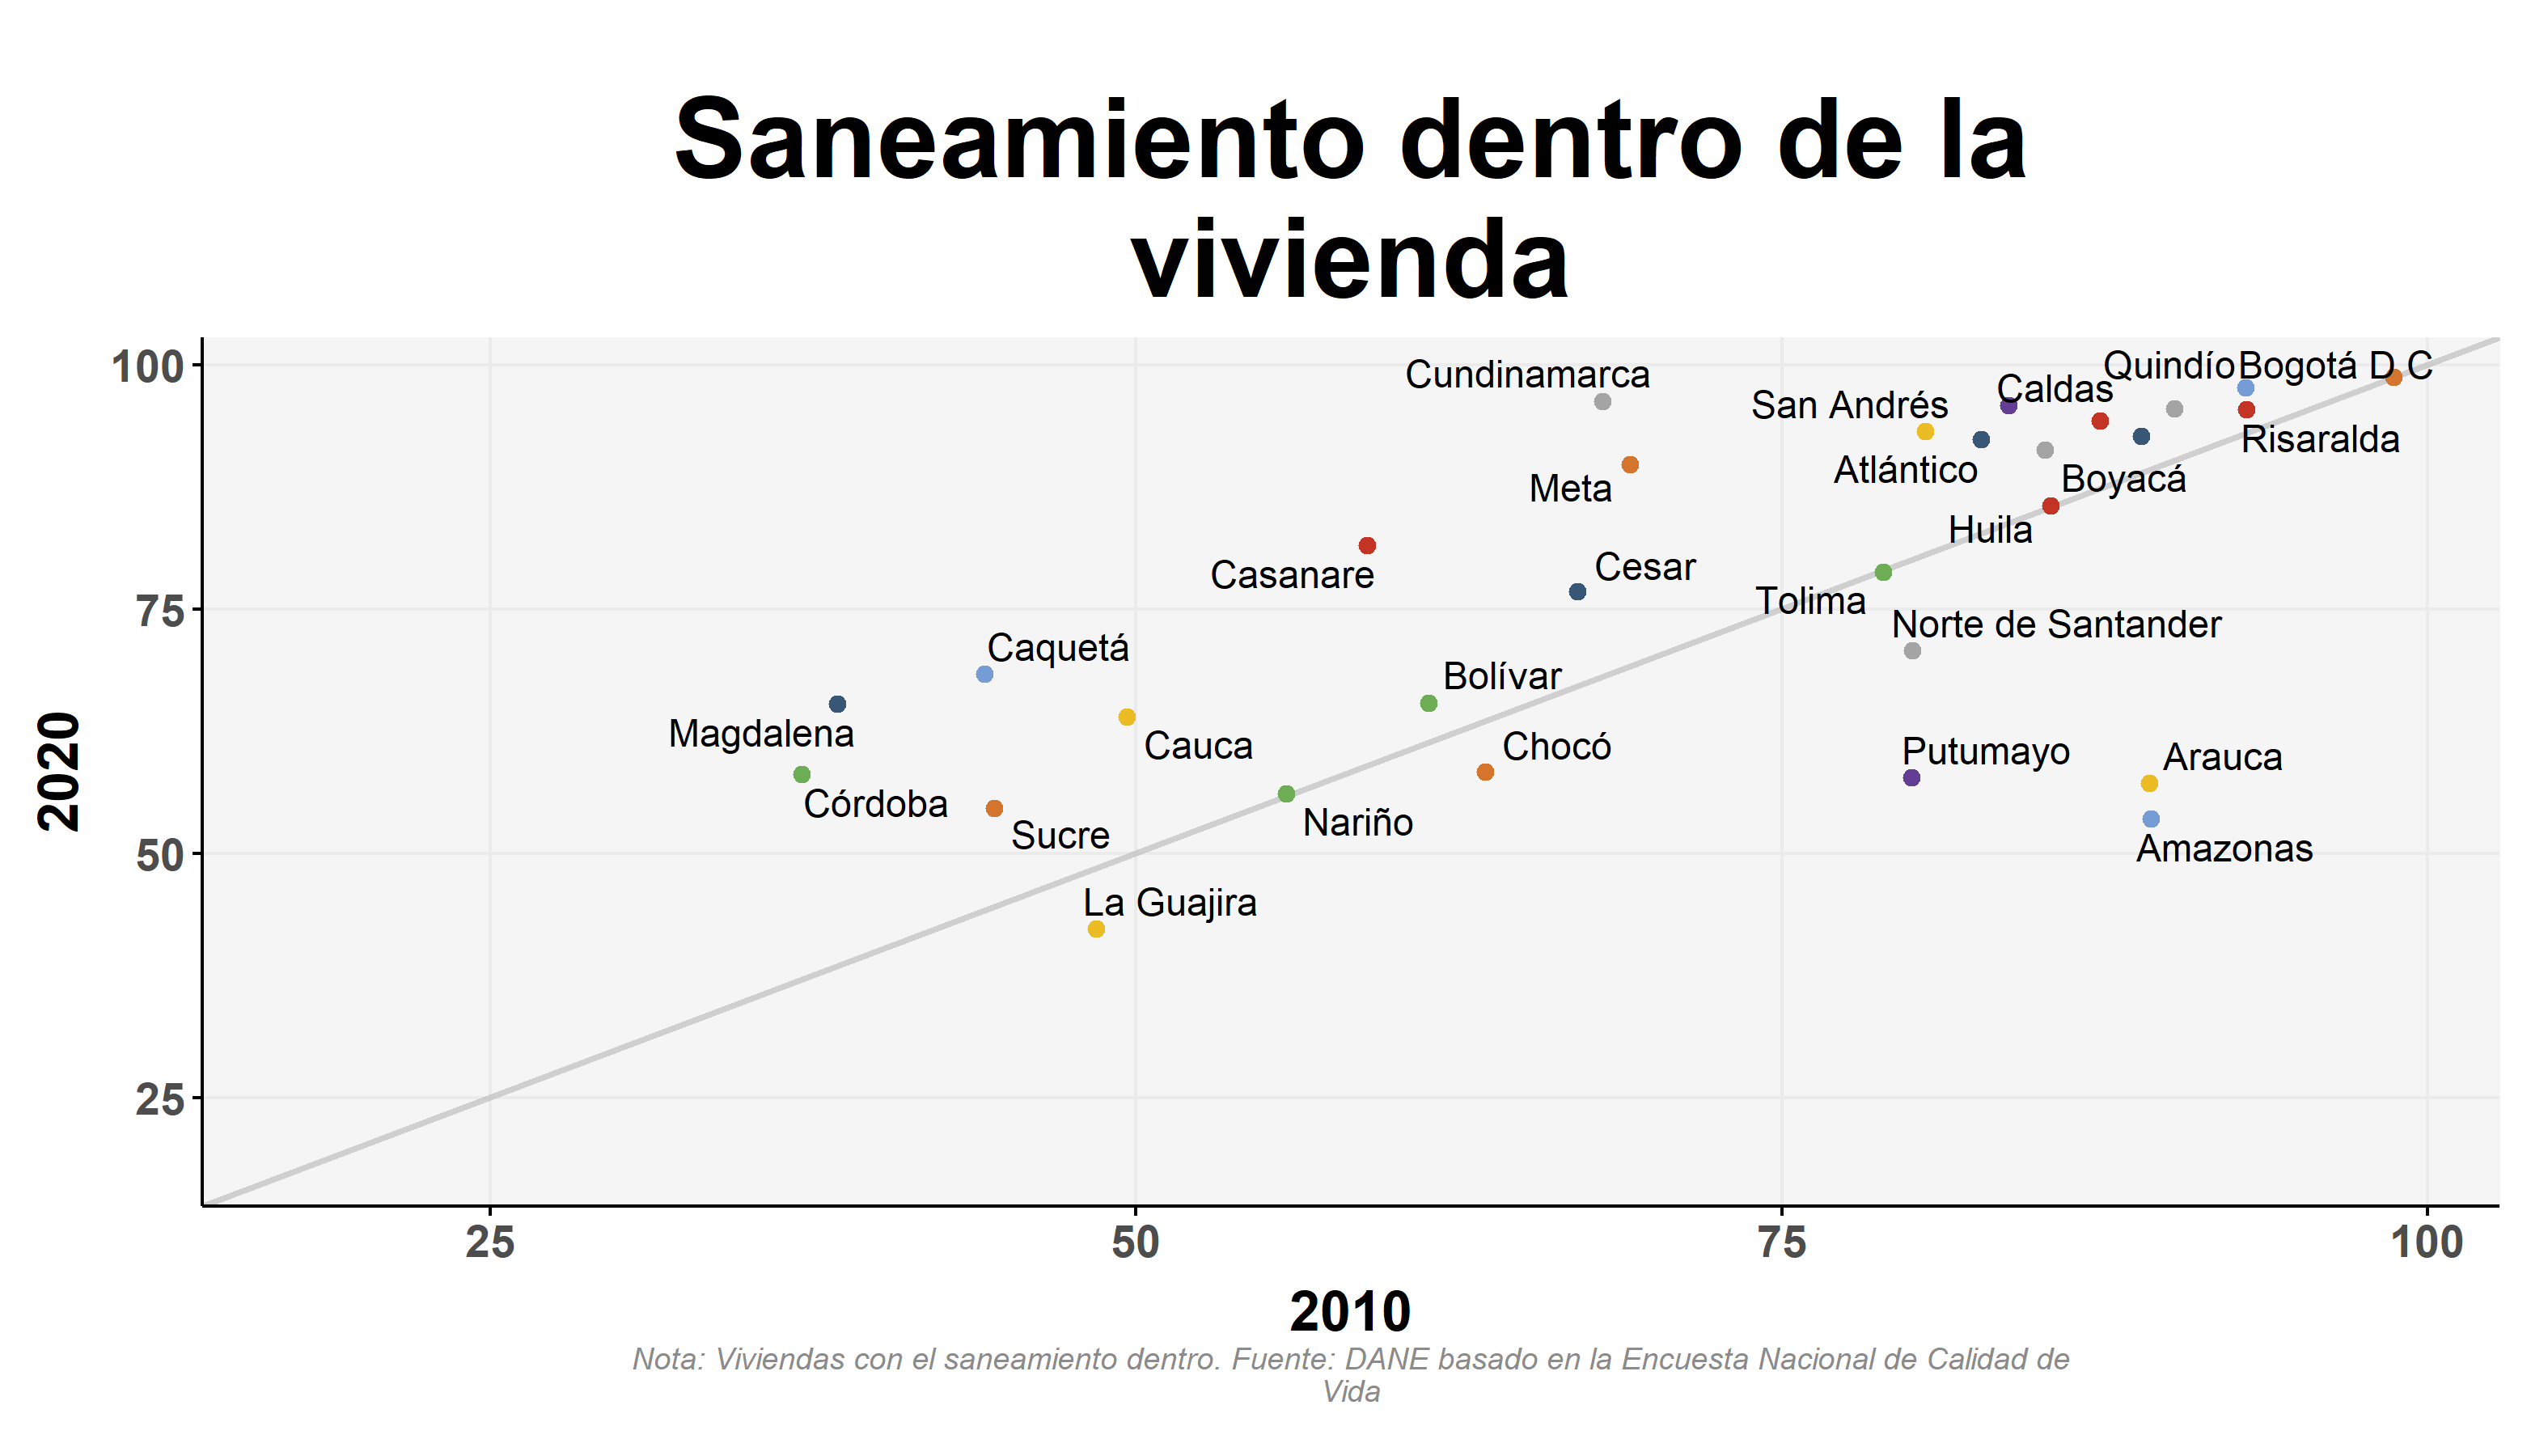
\includegraphics[width=\columnwidth]{img/var_193_scatter_time.png}
            \end{imagecolumn}
            \begin{textcolumn}
                \begin{itemize}
                    \item En promedio el acceso a saneamiento básico ha mejorado
                    \item Pero en algunos departamentos como La Guajira, Sucre y Amazonas, el acceso a saneamiento es bajo y persistente. 
                \end{itemize}
            \end{textcolumn}

    \printcolumns
    \end{slide}
    
    
    %%% ----------------------------
    %%% Características del hogar
    %%% ----------------------------
    \subsection{Crecimiento Económico}
    
        %%%-- Diversidad económica 
    \begin{slide}{8} 
                      \begin{imagecolumn}
                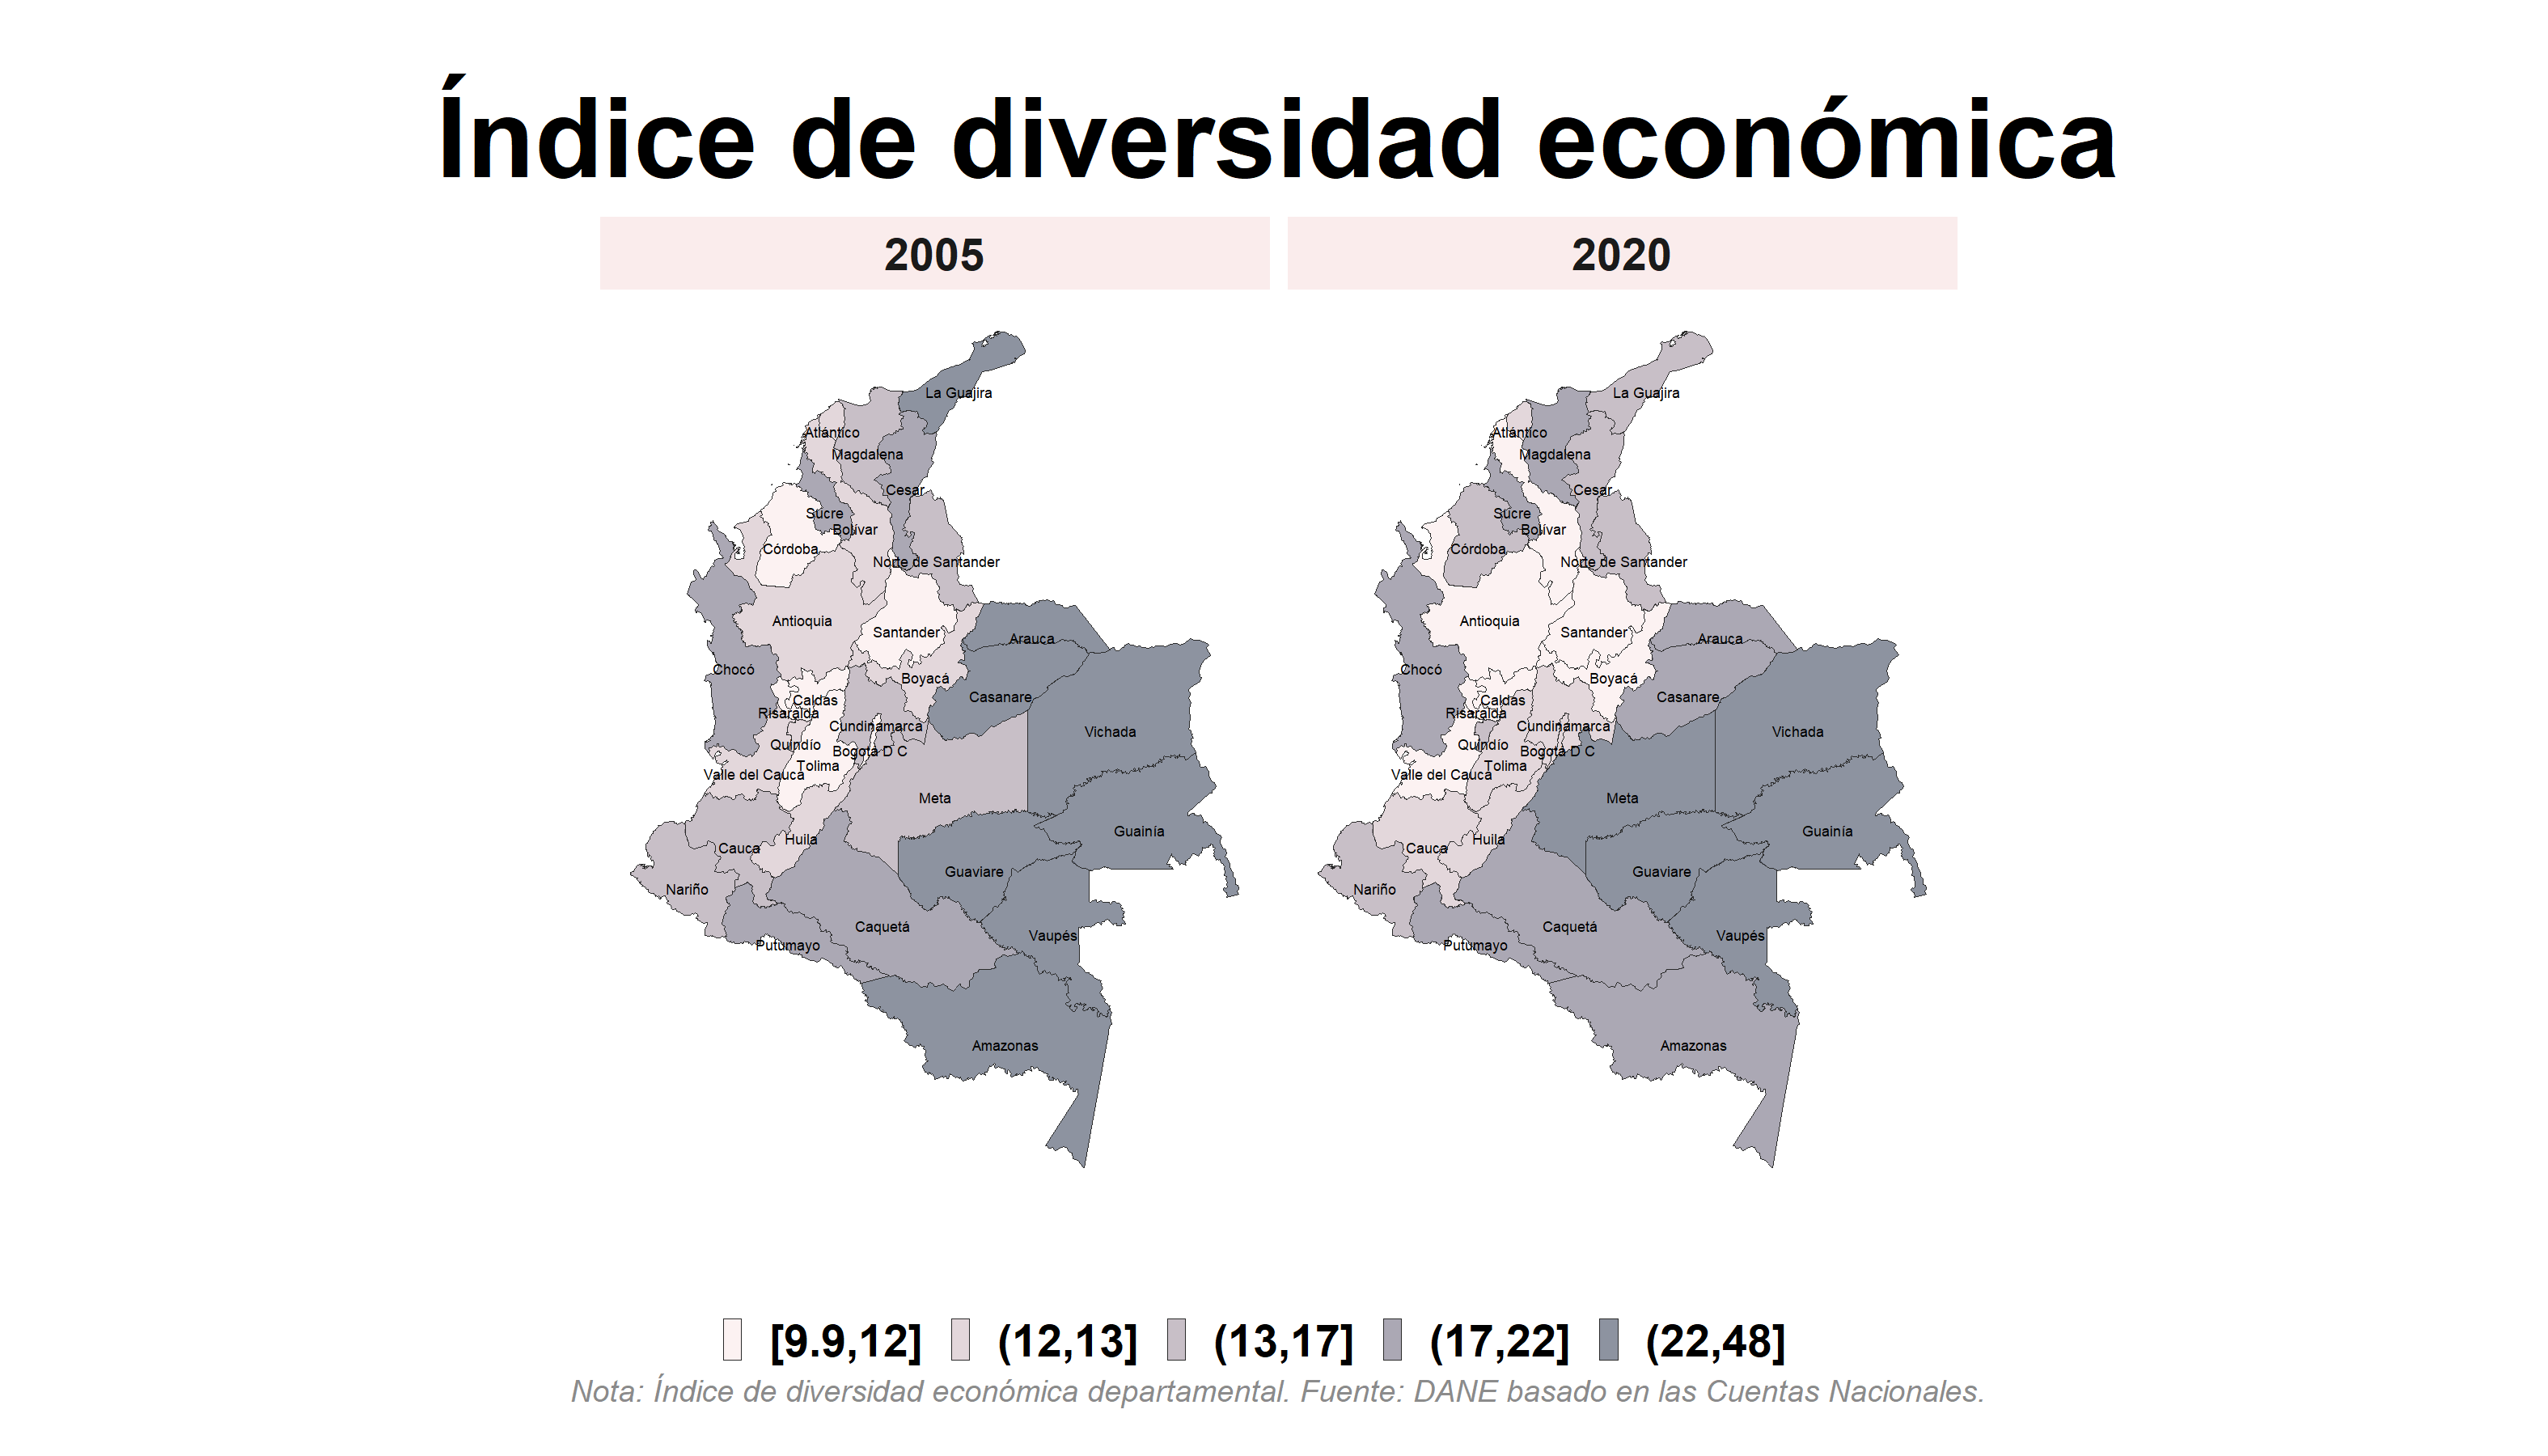
\includegraphics[width=\columnwidth]{img/var_300_map.png}
            \end{imagecolumn}
            \begin{textcolumn}
                \begin{itemize}
                    \item Las regiones son ahora más diversas en términos de actividad económica.
                    \item Pero en los departamentos más marginados persiste una alta dependencia de ciertos sectores
                \end{itemize}
            \end{textcolumn}

    \printcolumns
    \end{slide}
    
    
            %%%-- Highlights 
    \begin{slide}{8} 
            \begin{imagecolumn}
                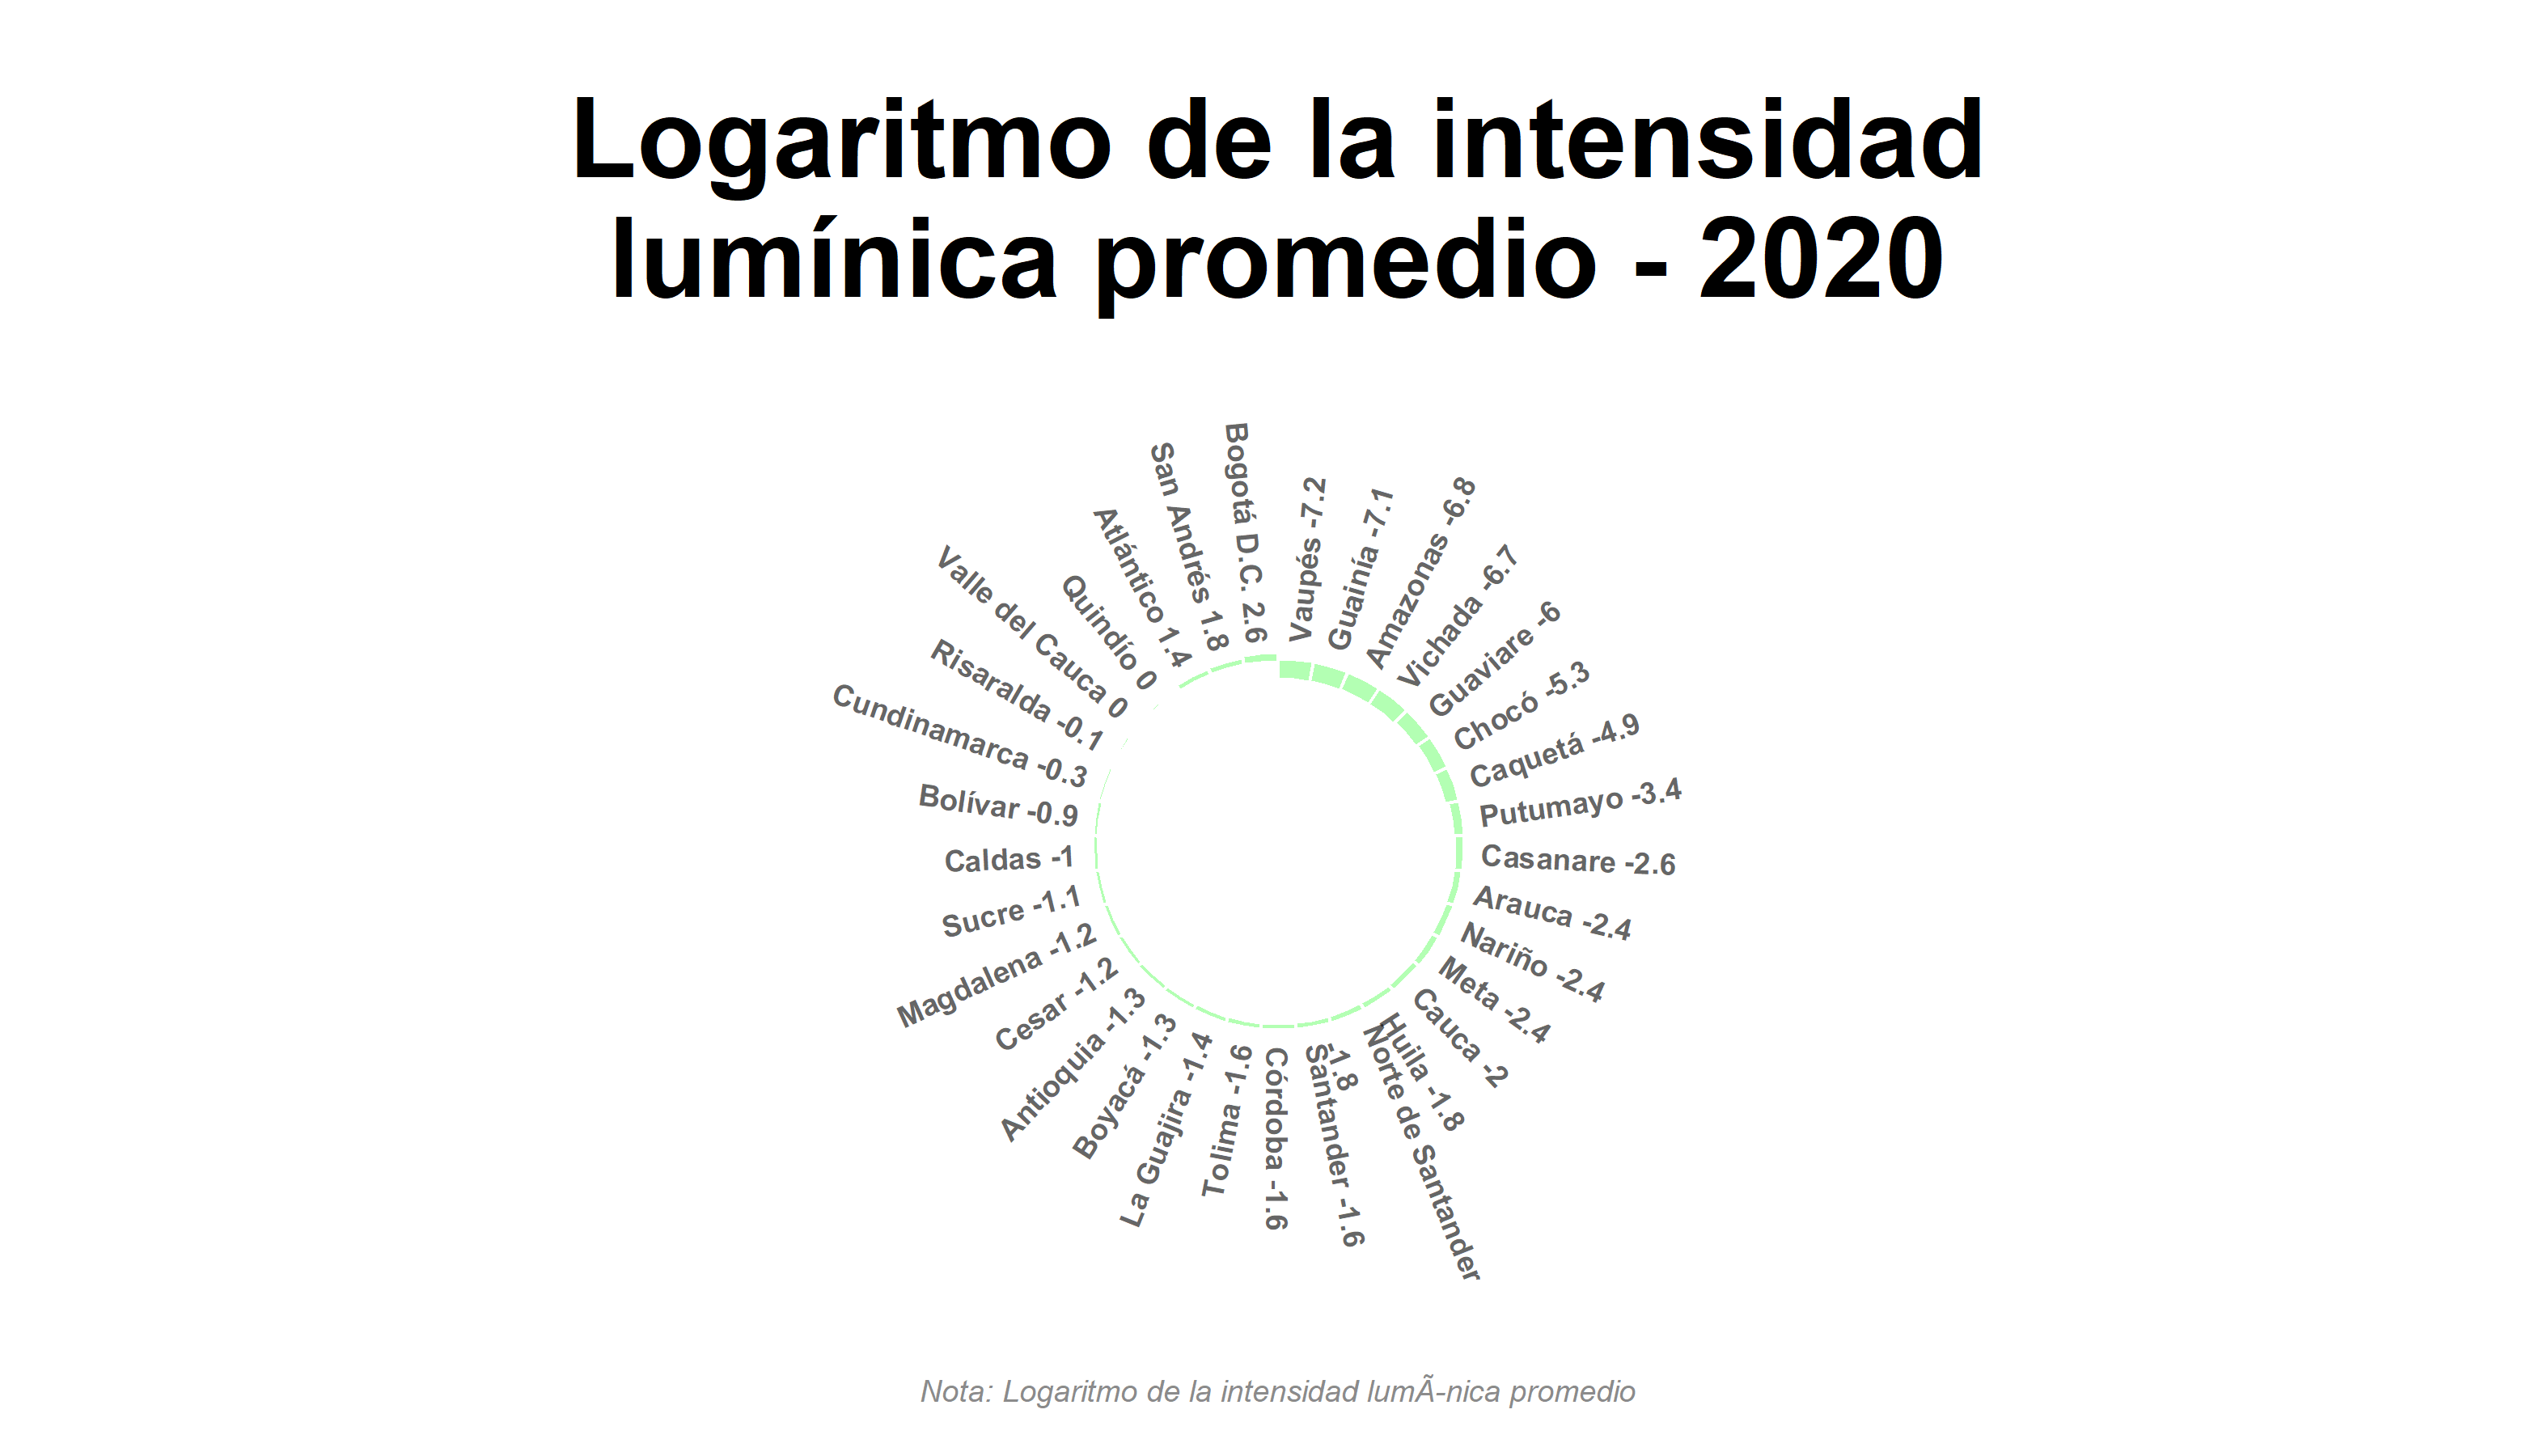
\includegraphics[width=\columnwidth]{img/var_301_static.png}
            \end{imagecolumn}
            \begin{textcolumn}
                \begin{itemize}
                    \item El índice de luminosidad confirma la heterogeneidad en actividad económica entre regiones.
                \end{itemize}
            \end{textcolumn}

    \printcolumns
    \end{slide}
    
    
    %%% ----------------------------
    %%% Migracion
    %%% ----------------------------
    \subsection{Migración}
    
        %%%-- Highlights 
    \begin{slide}{10} 
                      \begin{imagecolumn}
                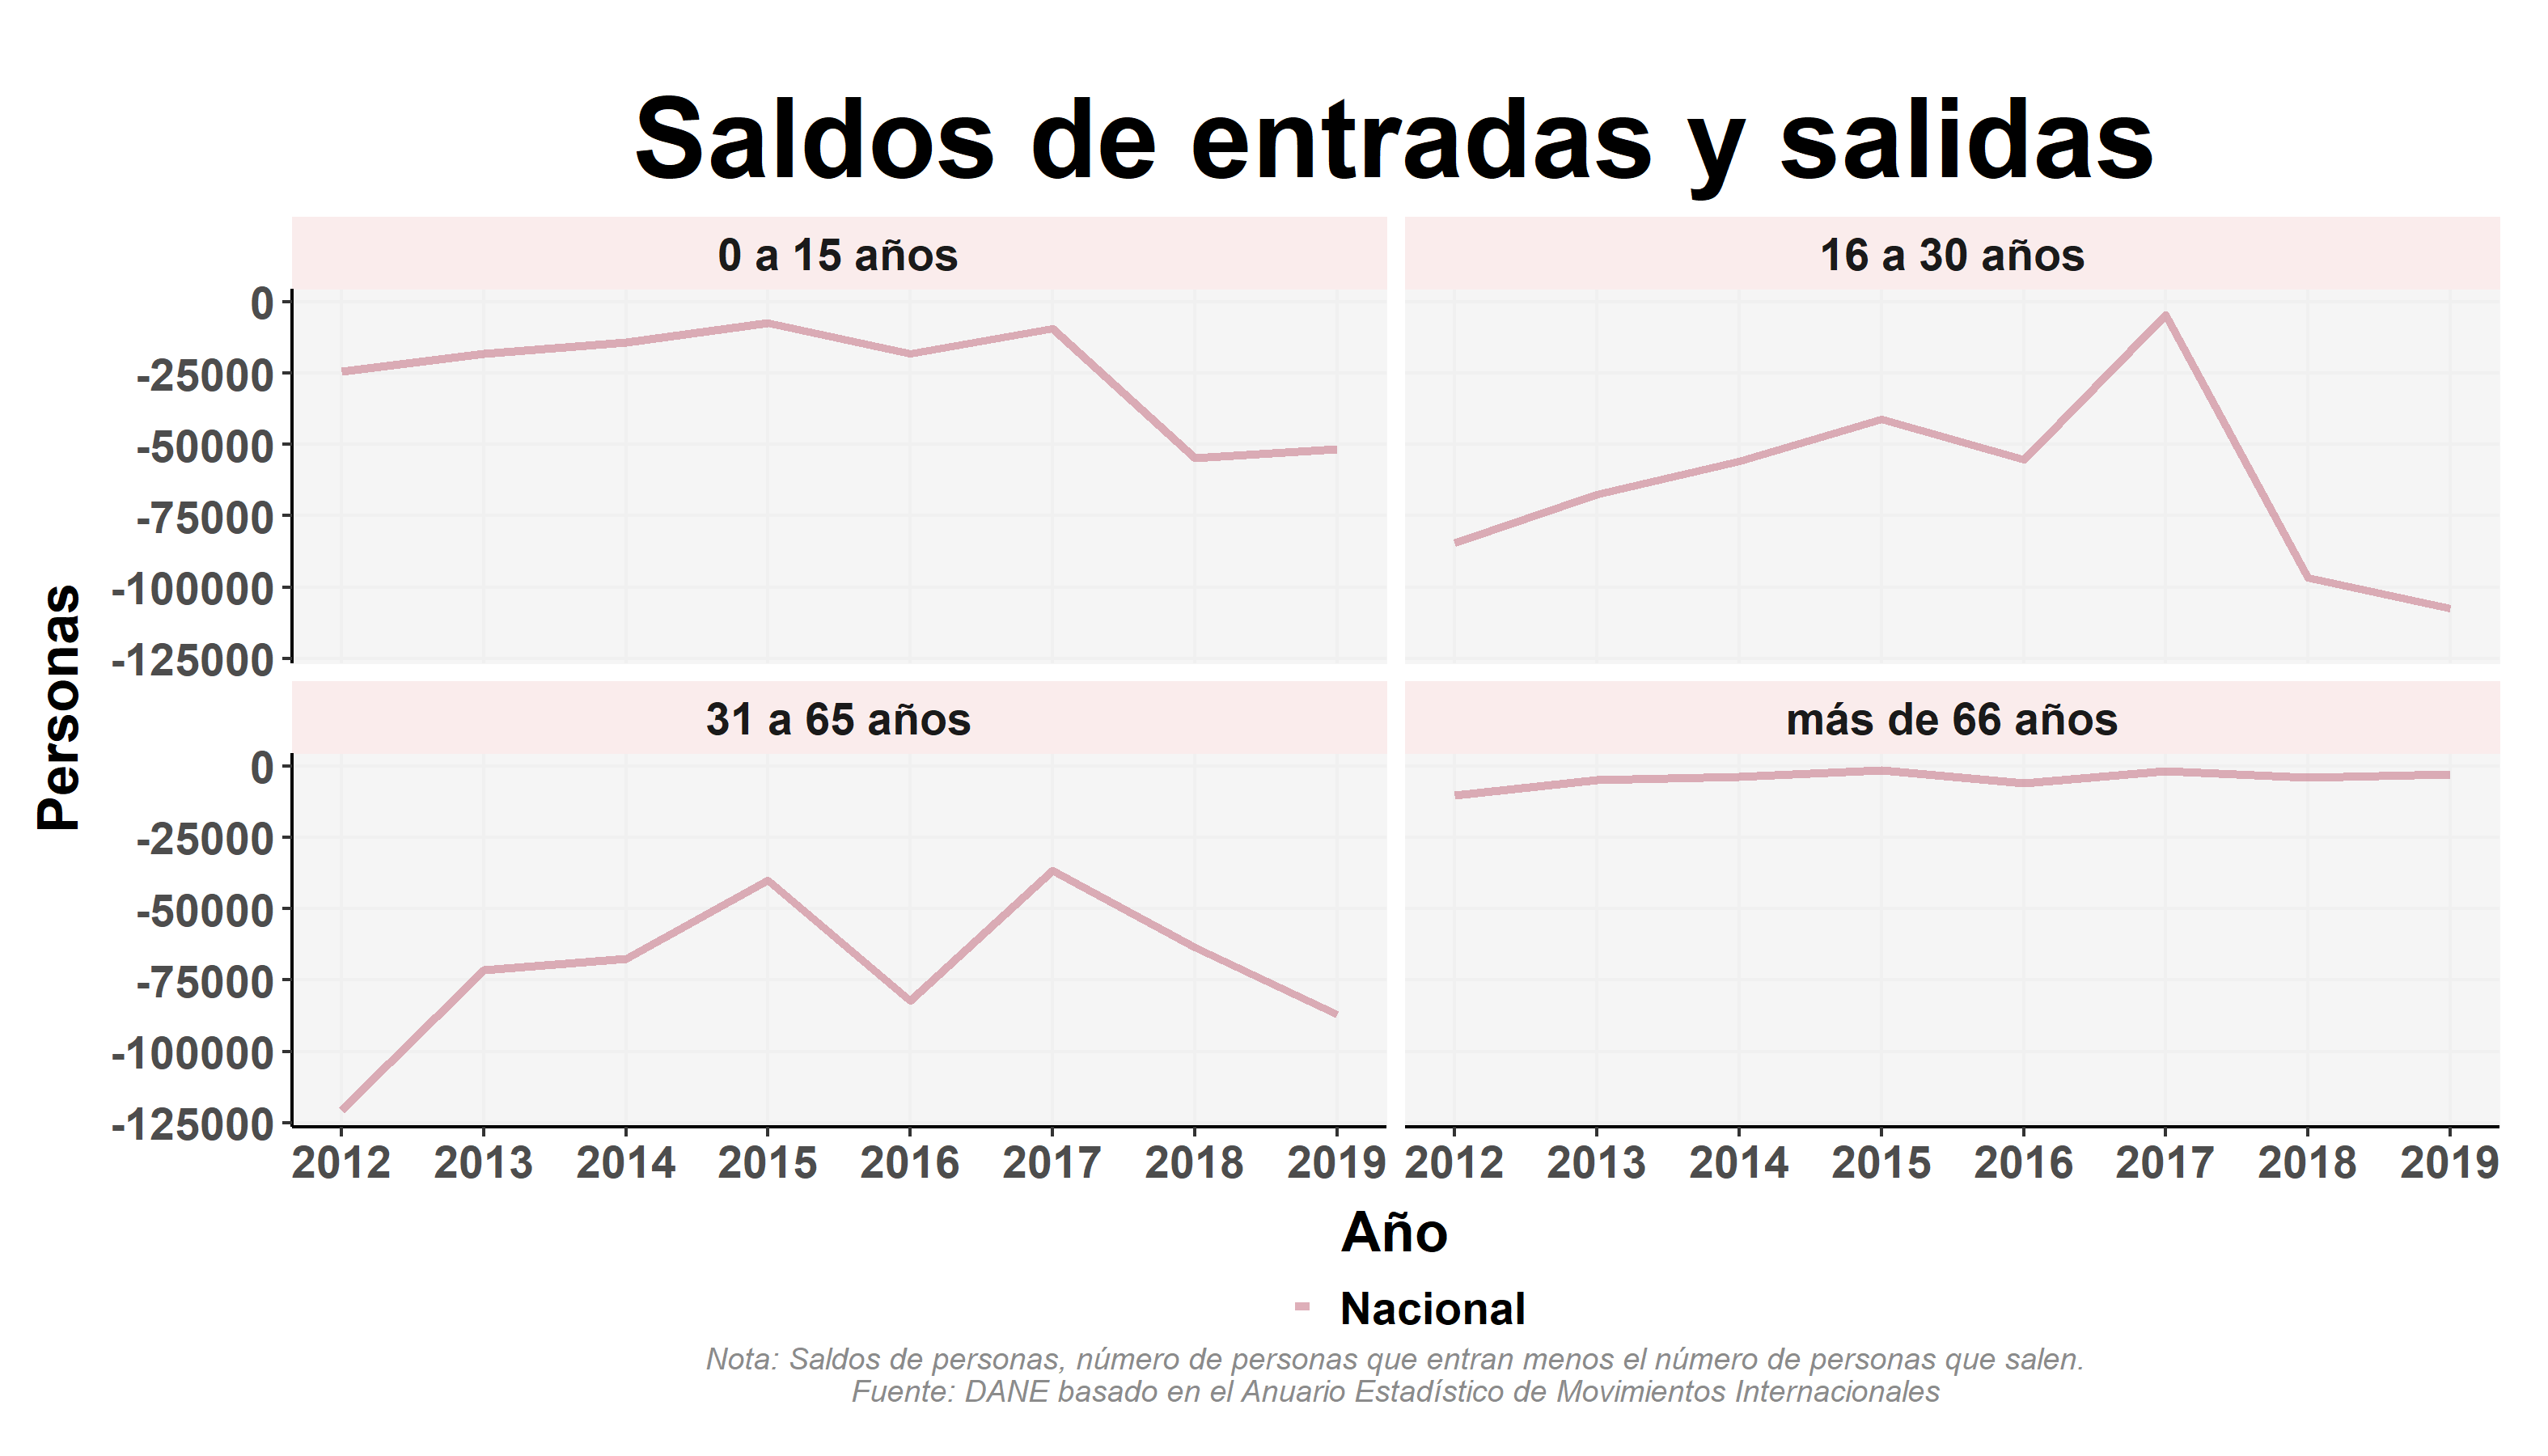
\includegraphics[width=\columnwidth]{img/var_238_trend.png}
            \end{imagecolumn}
            \begin{textcolumn}
                \begin{itemize}
                    \item La crisis migratoria venezolana se concentró en el grupo de edad entre los 16-55 años.
                \end{itemize}
            \end{textcolumn}

    \printcolumns
    \end{slide}
    
    %%% ----------------------------
    %%% Cambio Climático
    %%% ----------------------------
    \subsection{Cambio Climático}
    
        %%%-- Highlights 
    \begin{slide}{11} 
                      \begin{imagecolumn}
                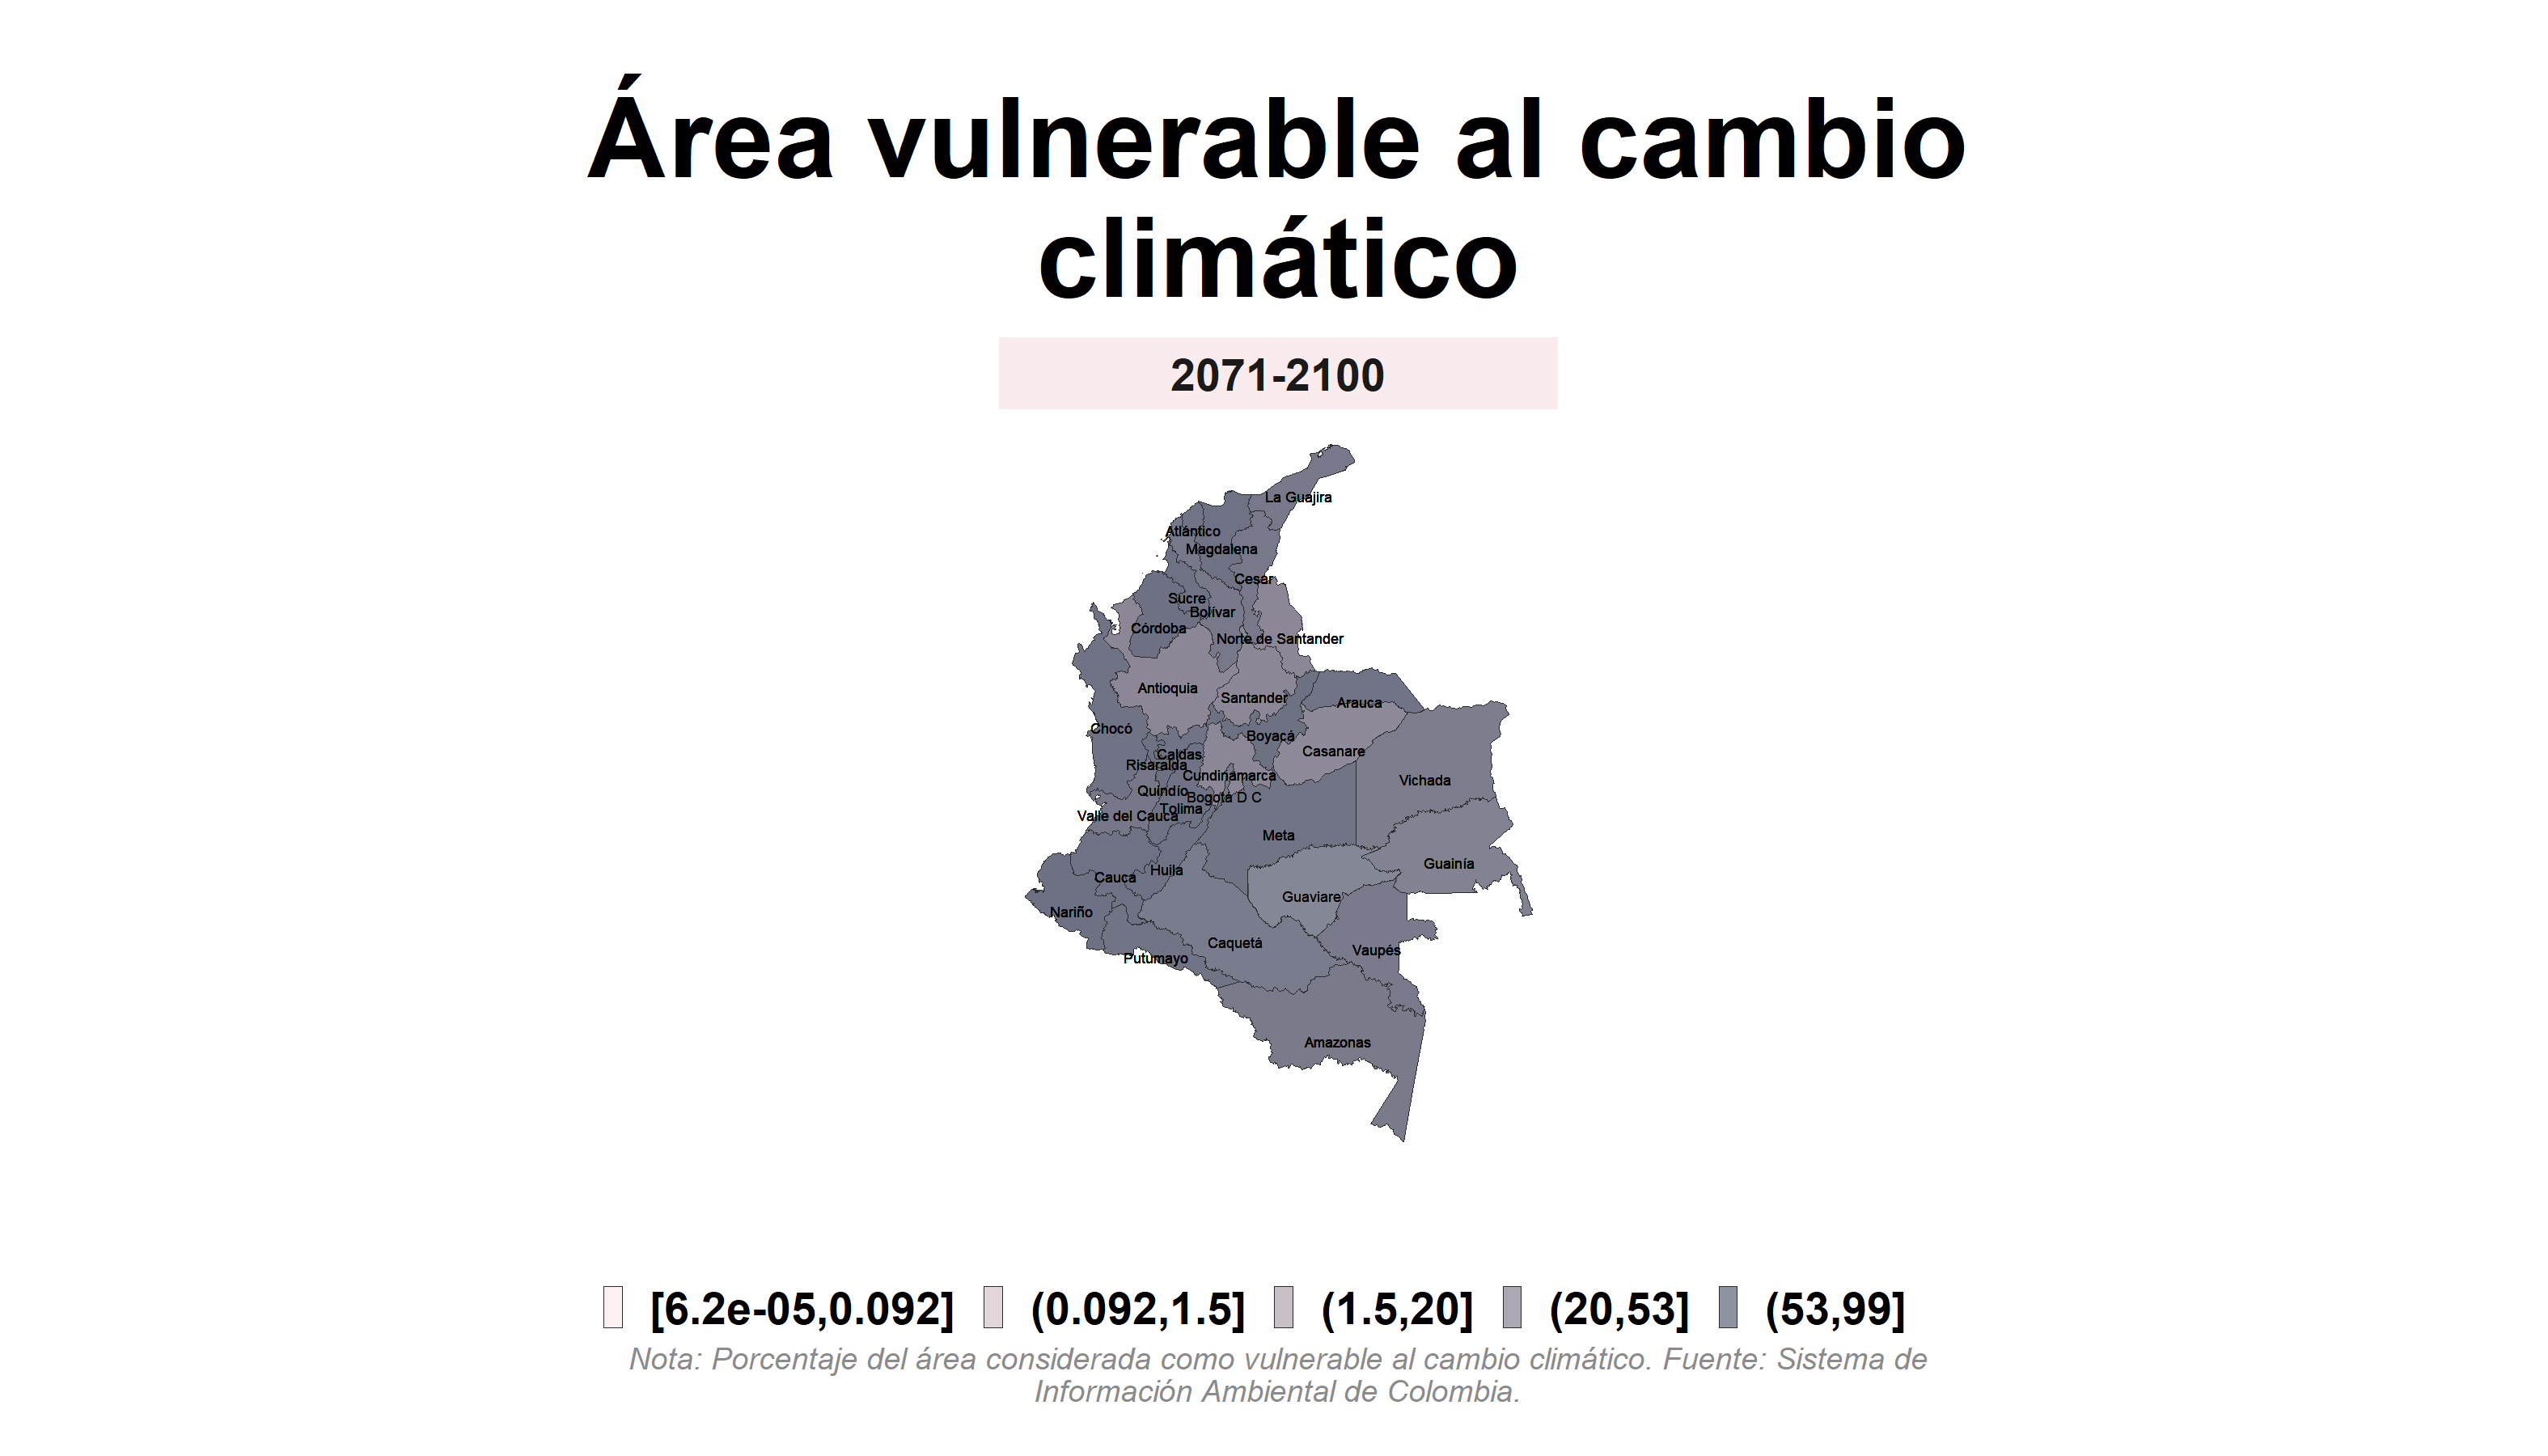
\includegraphics[width=\columnwidth]{img/var_299_map.png}
            \end{imagecolumn}
            \begin{textcolumn}
                \begin{itemize}
                    \item El impacto del cambio climático tendrá efectos diferenciados en las regiones del país
                    \item Las regiones costeras serán las más impactadas
                \end{itemize}
            \end{textcolumn}

    \printcolumns
    \end{slide}
    
        %%% ----------------------------
    %%% Indicadores de resultados
    %%% ----------------------------
    
     \section{Resultados}
    %%% Resultados
    \slidetitle{12}
    
        %%% ----------------------------
    %%% Infancia y Niñez
    %%% ----------------------------
    \subsection{Infancia y niñez}

        %%%-- Tasa de Mortalidad Infantil 
        \begin{slide}{13} 
                      \begin{imagecolumn}
                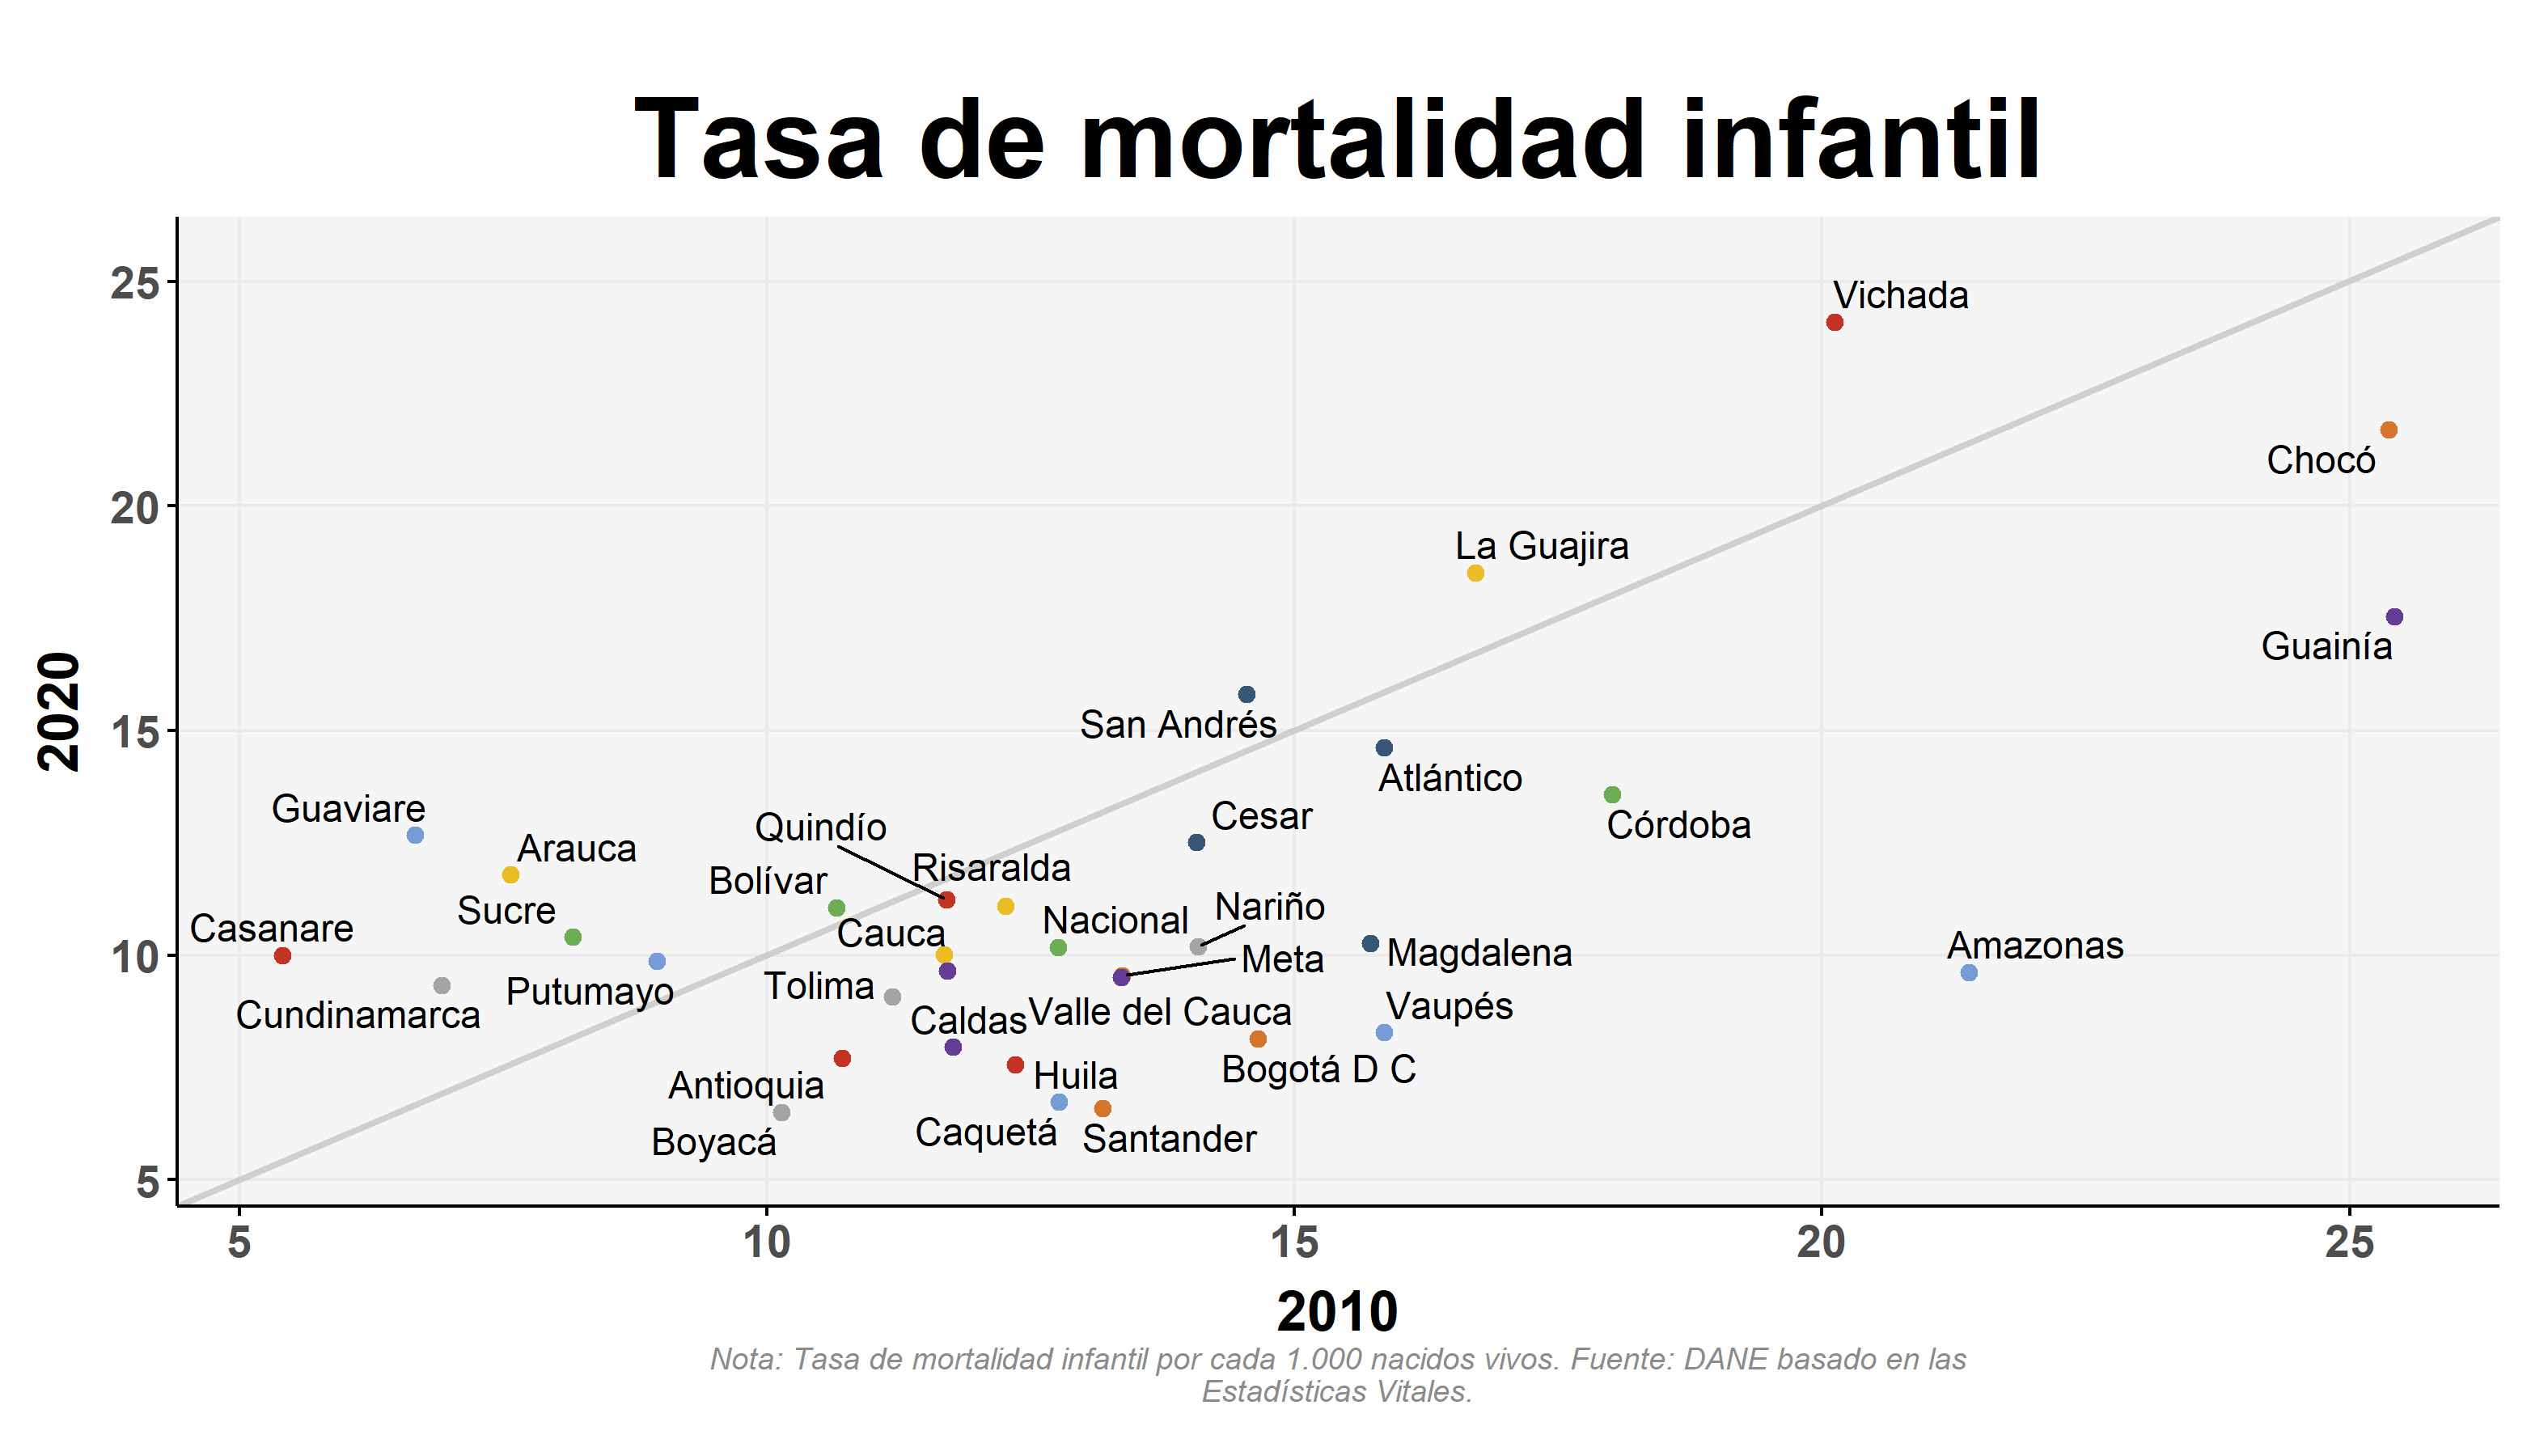
\includegraphics[width=\columnwidth]{img/var_290_scatter_time.png}
            \end{imagecolumn}
            \begin{textcolumn}
                \begin{itemize}
                    \item En la mayor parte de las regiones, la mortalidad infantil disminuyó entre 2010 y 2010. 
                    \item Pero todavía coexisten regiones con tasas de mortalidad infantil similares a las de Sur África (24%, Vichada) y a las de Estados Unidos (6%, Boyacá)                
                \end{itemize}
            \end{textcolumn}

    \printcolumns
    \end{slide}
  
      %%%-- Asistencia escolar menores 5 años
  
            \begin{slide}{13} 
                      \begin{imagecolumn}
                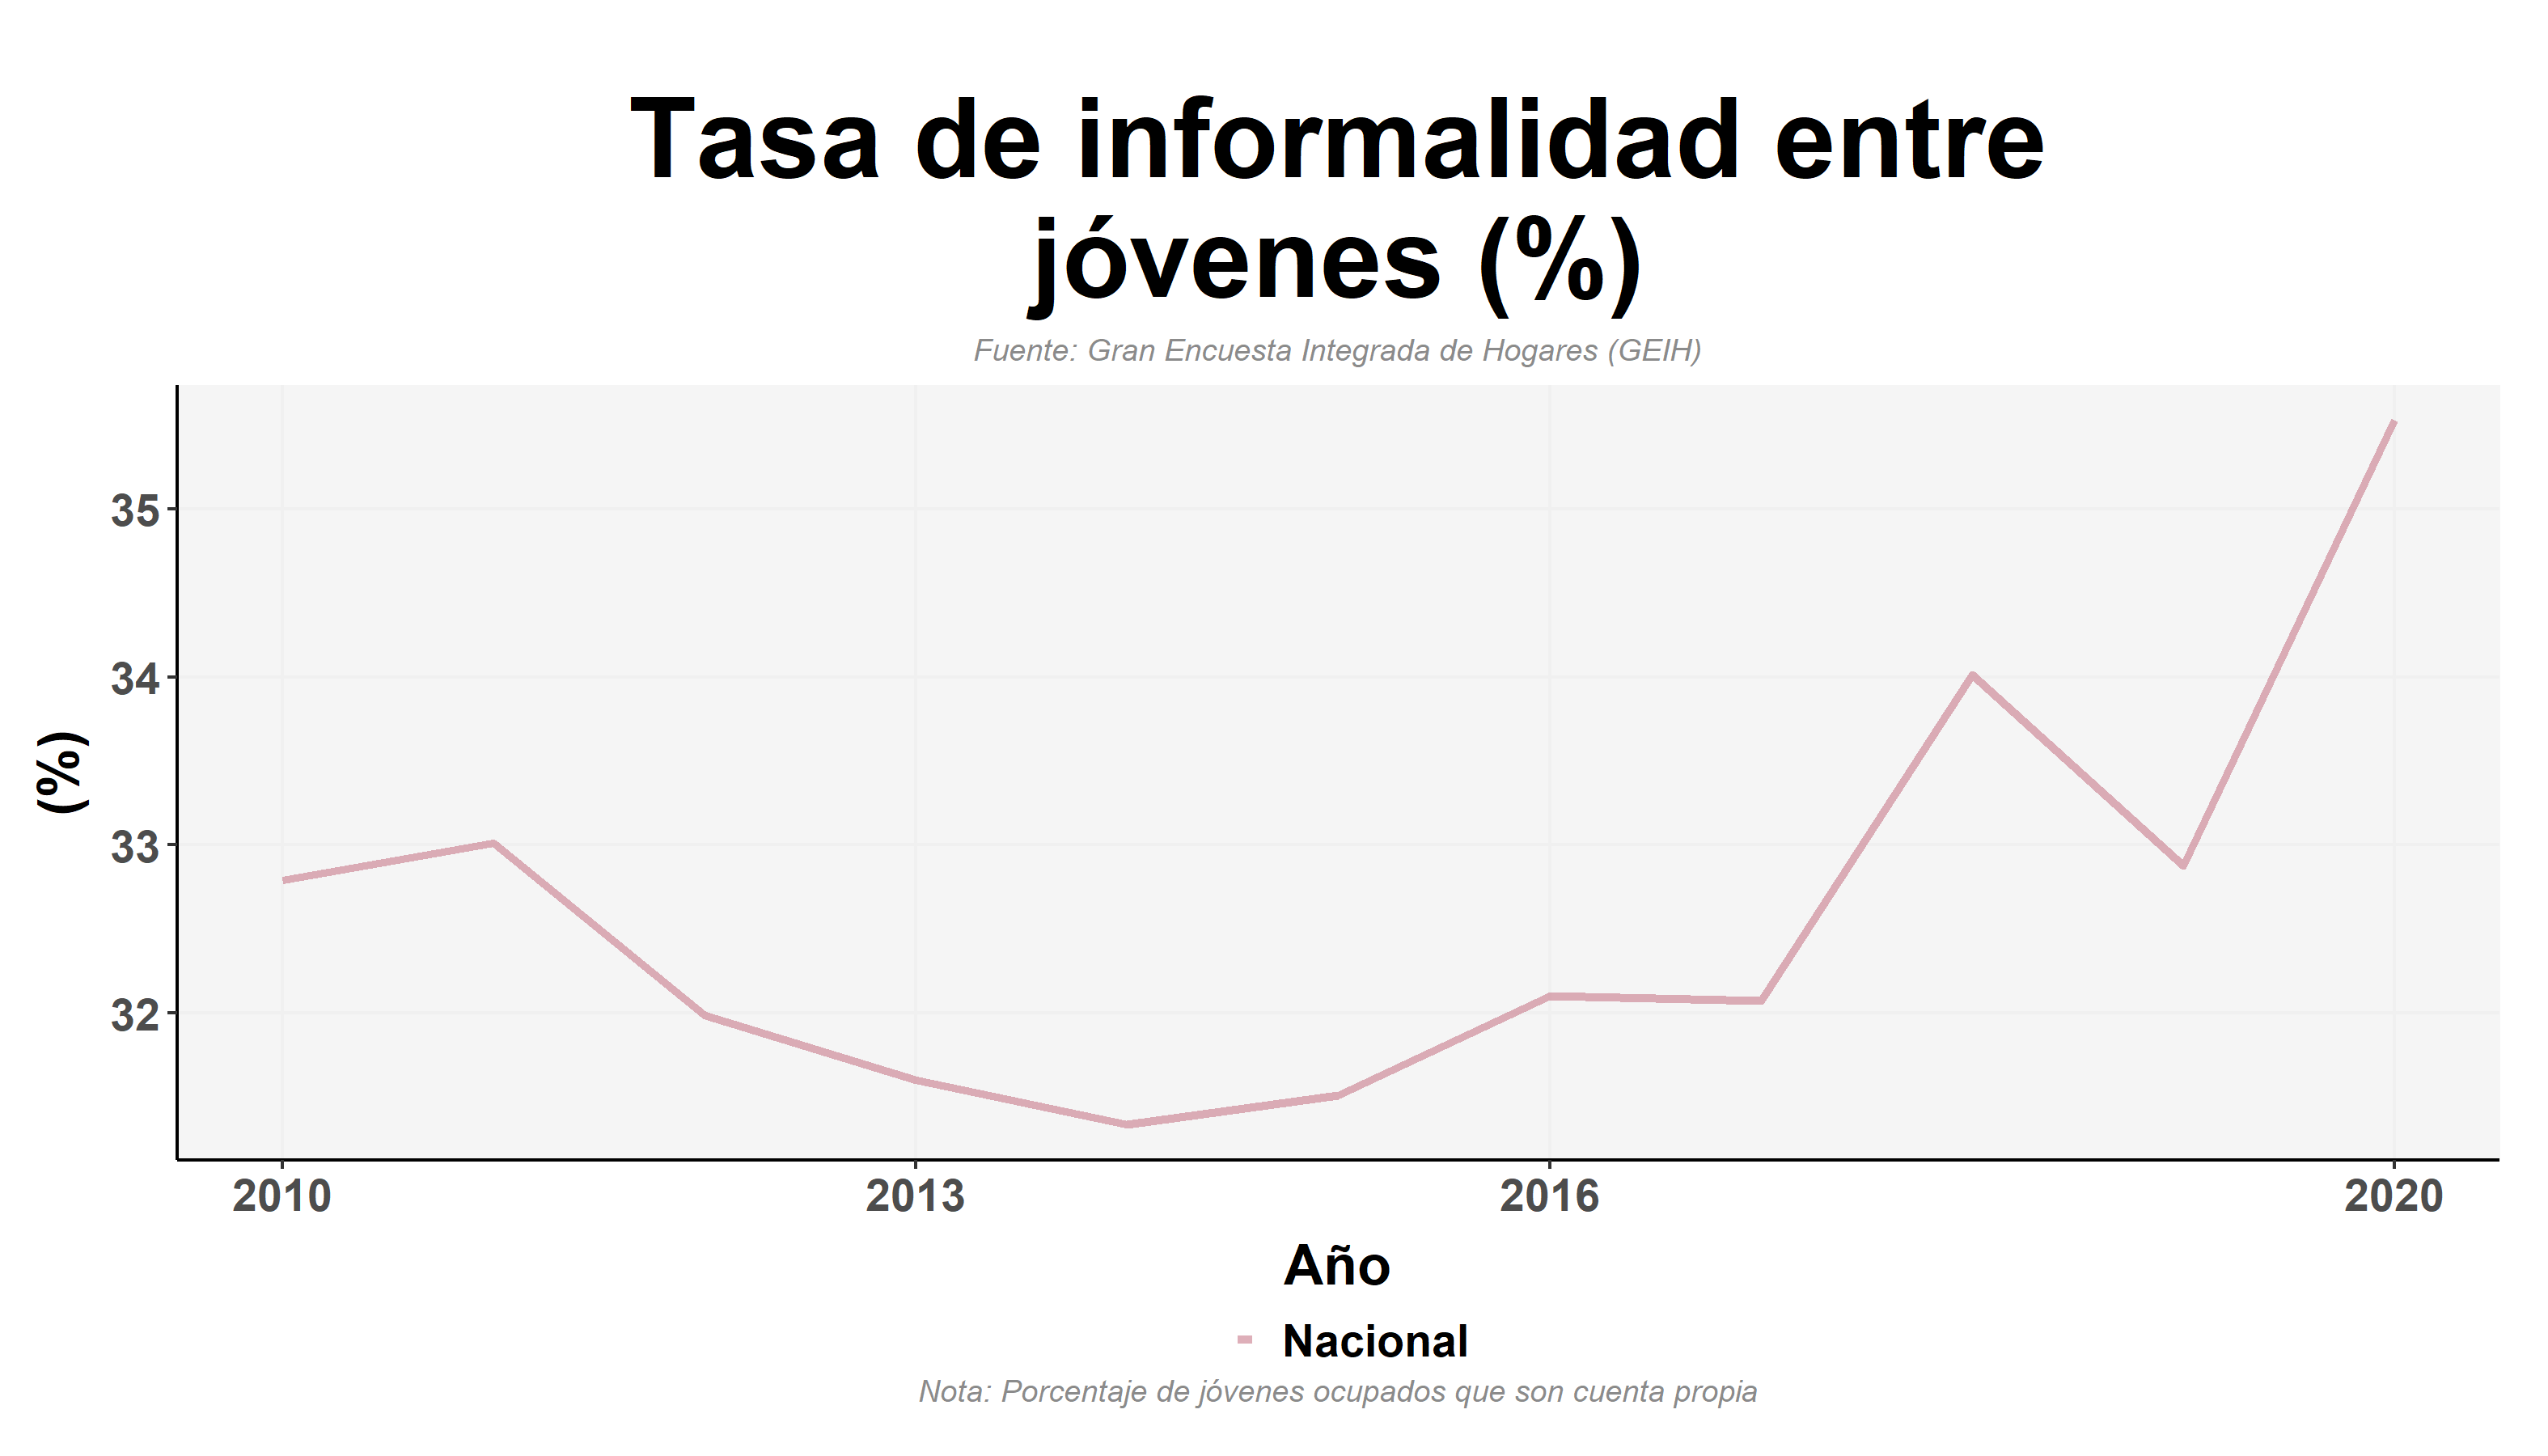
\includegraphics[width=\columnwidth]{img/var_100_trend.png}
            \end{imagecolumn}
            \begin{textcolumn}
                \begin{itemize}
                    \item La tasa de asistencia escolar entre menores de 5 años en zonas urbanas es casi el doble que en zonas rurales. 
                    \item Esta brecha se ha mantenido en el tiempo  
                    \item A excepción de 2020, donde la asistencia en cabeceras disminuyó drásticamente, cerrando la brecha.
                \end{itemize}
            \end{textcolumn}

    \printcolumns
    \end{slide}

          %%%-- Tamaño de clase primaria
  
            \begin{slide}{13} 
                      \begin{imagecolumn}
                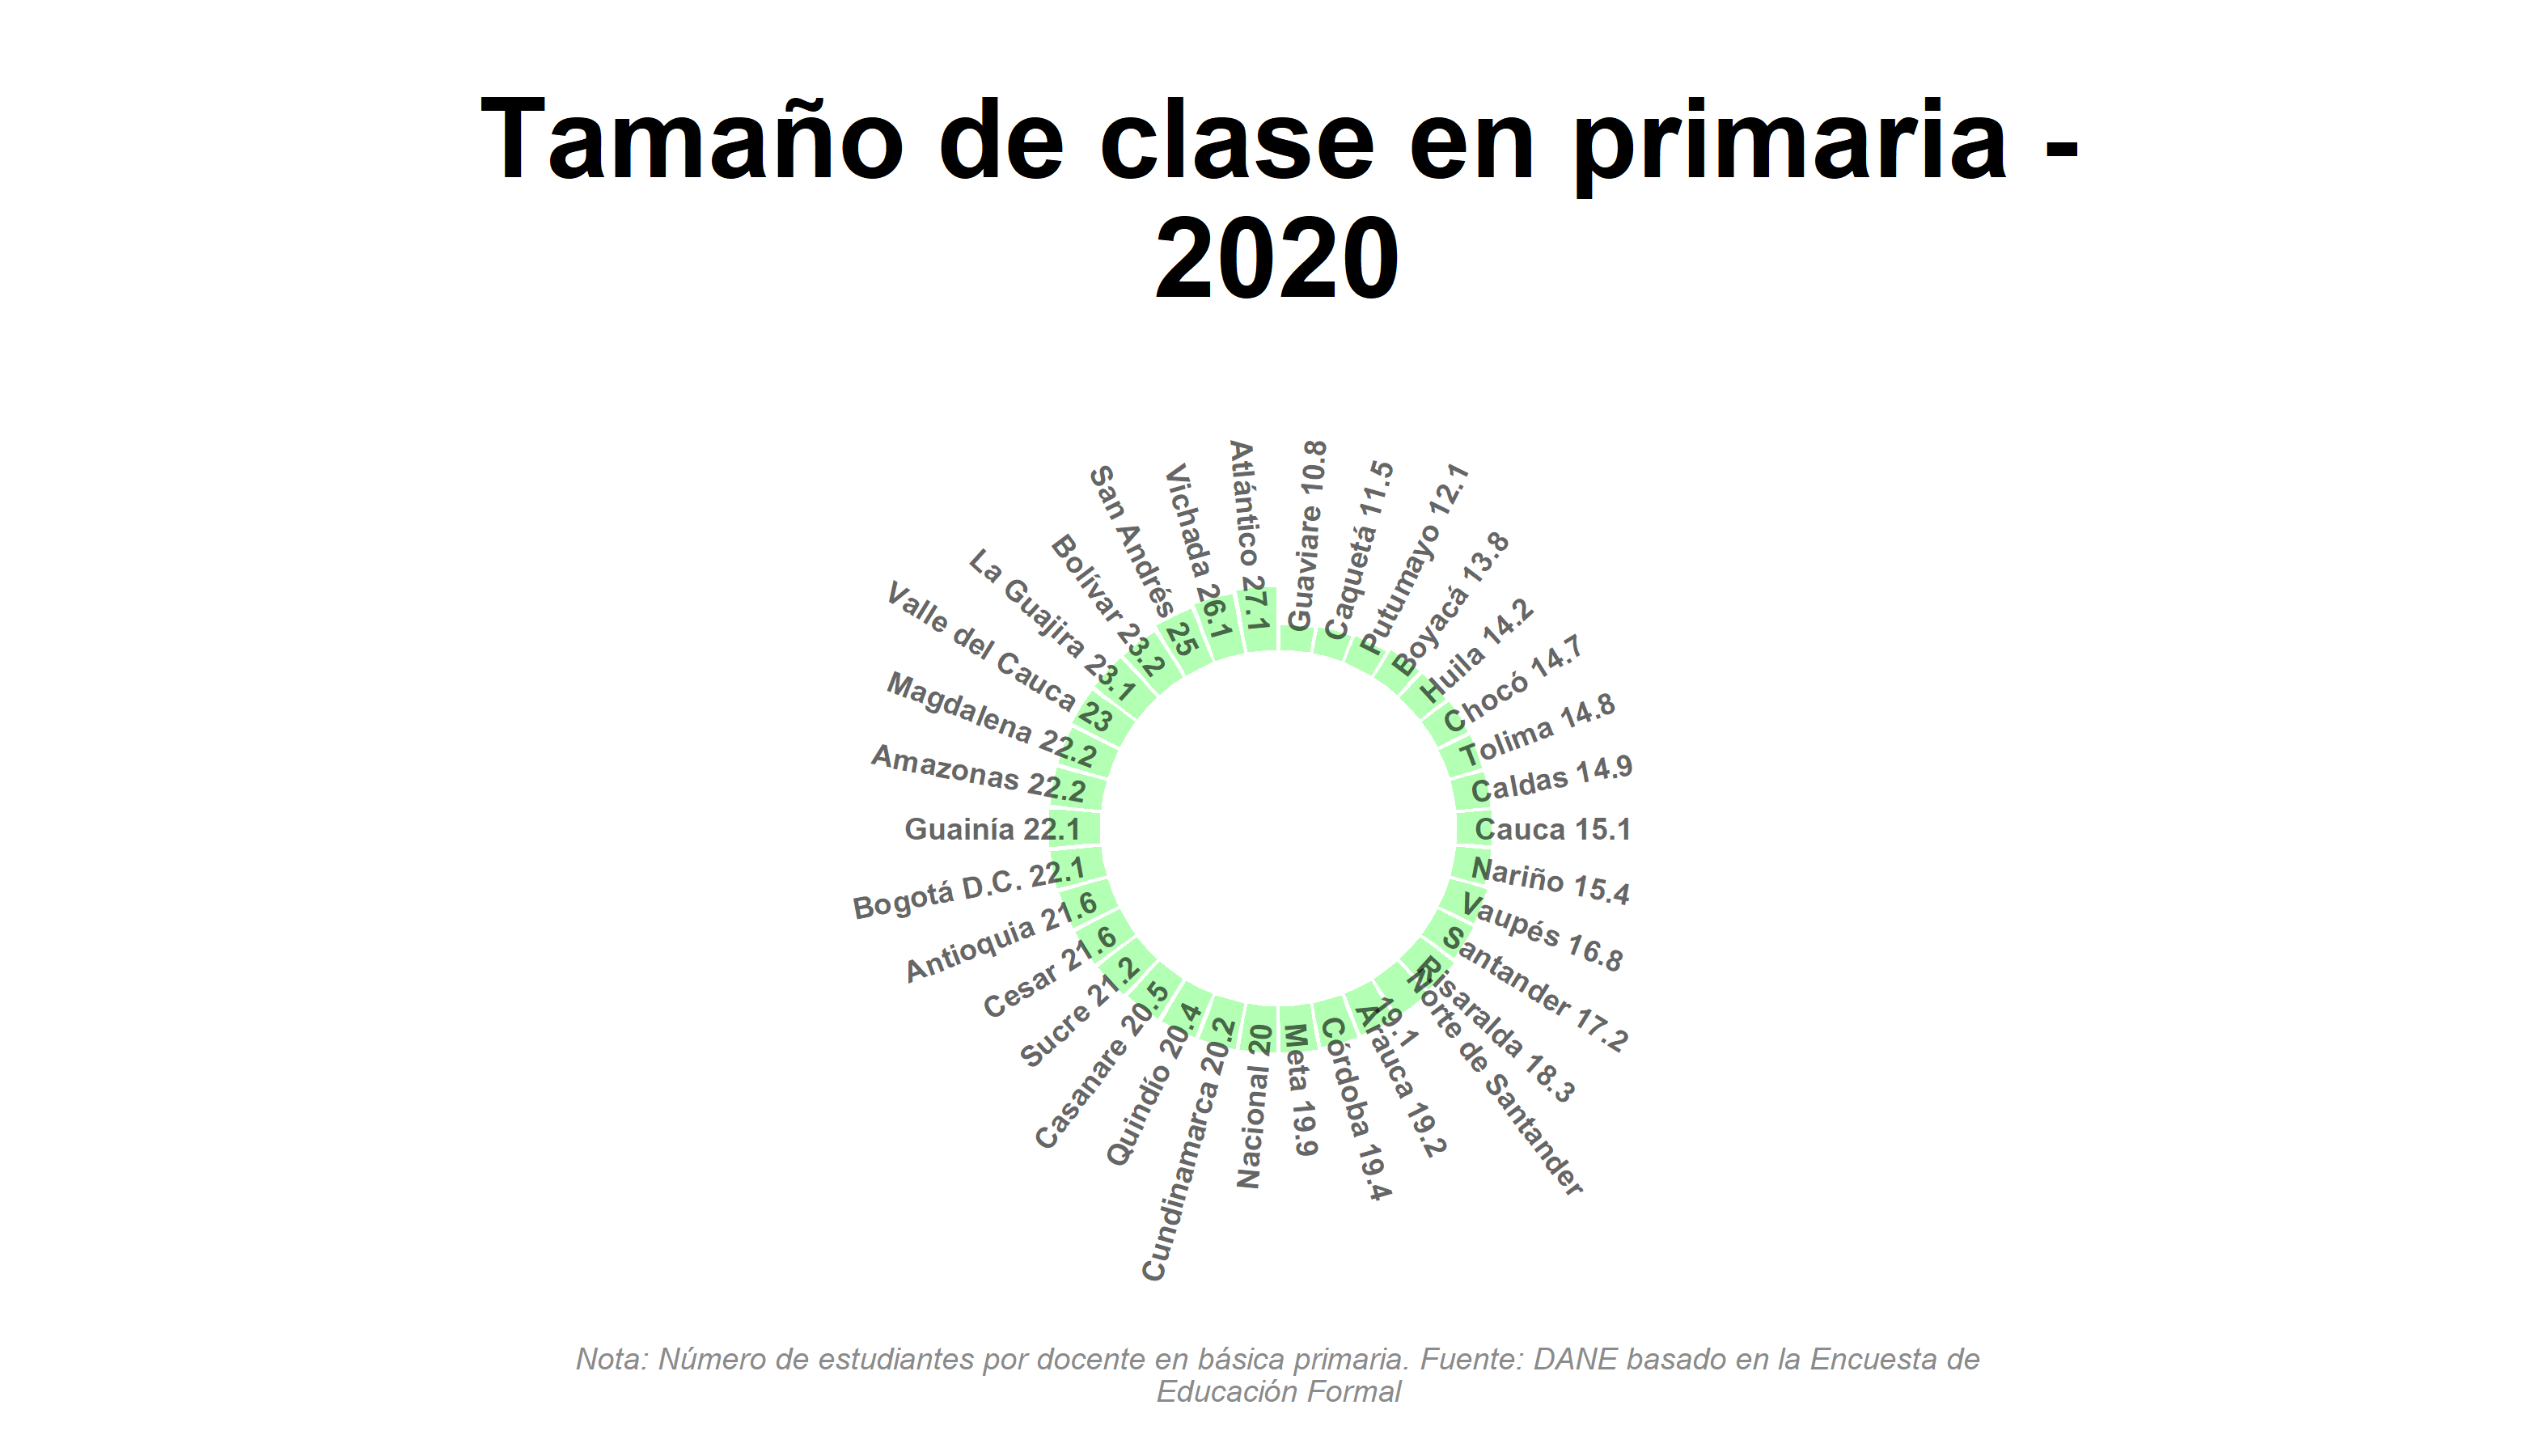
\includegraphics[width=\columnwidth]{img/var_228_static.png}
            \end{imagecolumn}
            \begin{textcolumn}
                \begin{itemize}
                    \item Hay una gran variación geográfica en la calidad de la educación primaria, medida como el tamaño de clase. 
                    \item Coexisten regiones con 27 estudiantes por docente (Atlántico) junto con regiones con tan sólo 12 estudiantes por docente (Guaviare)  
                \end{itemize}
            \end{textcolumn}

    \printcolumns
    \end{slide}
    
    
      %%% ----------------------------
    %%% Juventud
    %%% ----------------------------
    \subsection{Juventud}
    
    %%%-- Educación Superior
    \begin{slide}{14} 
                      \begin{imagecolumn}
                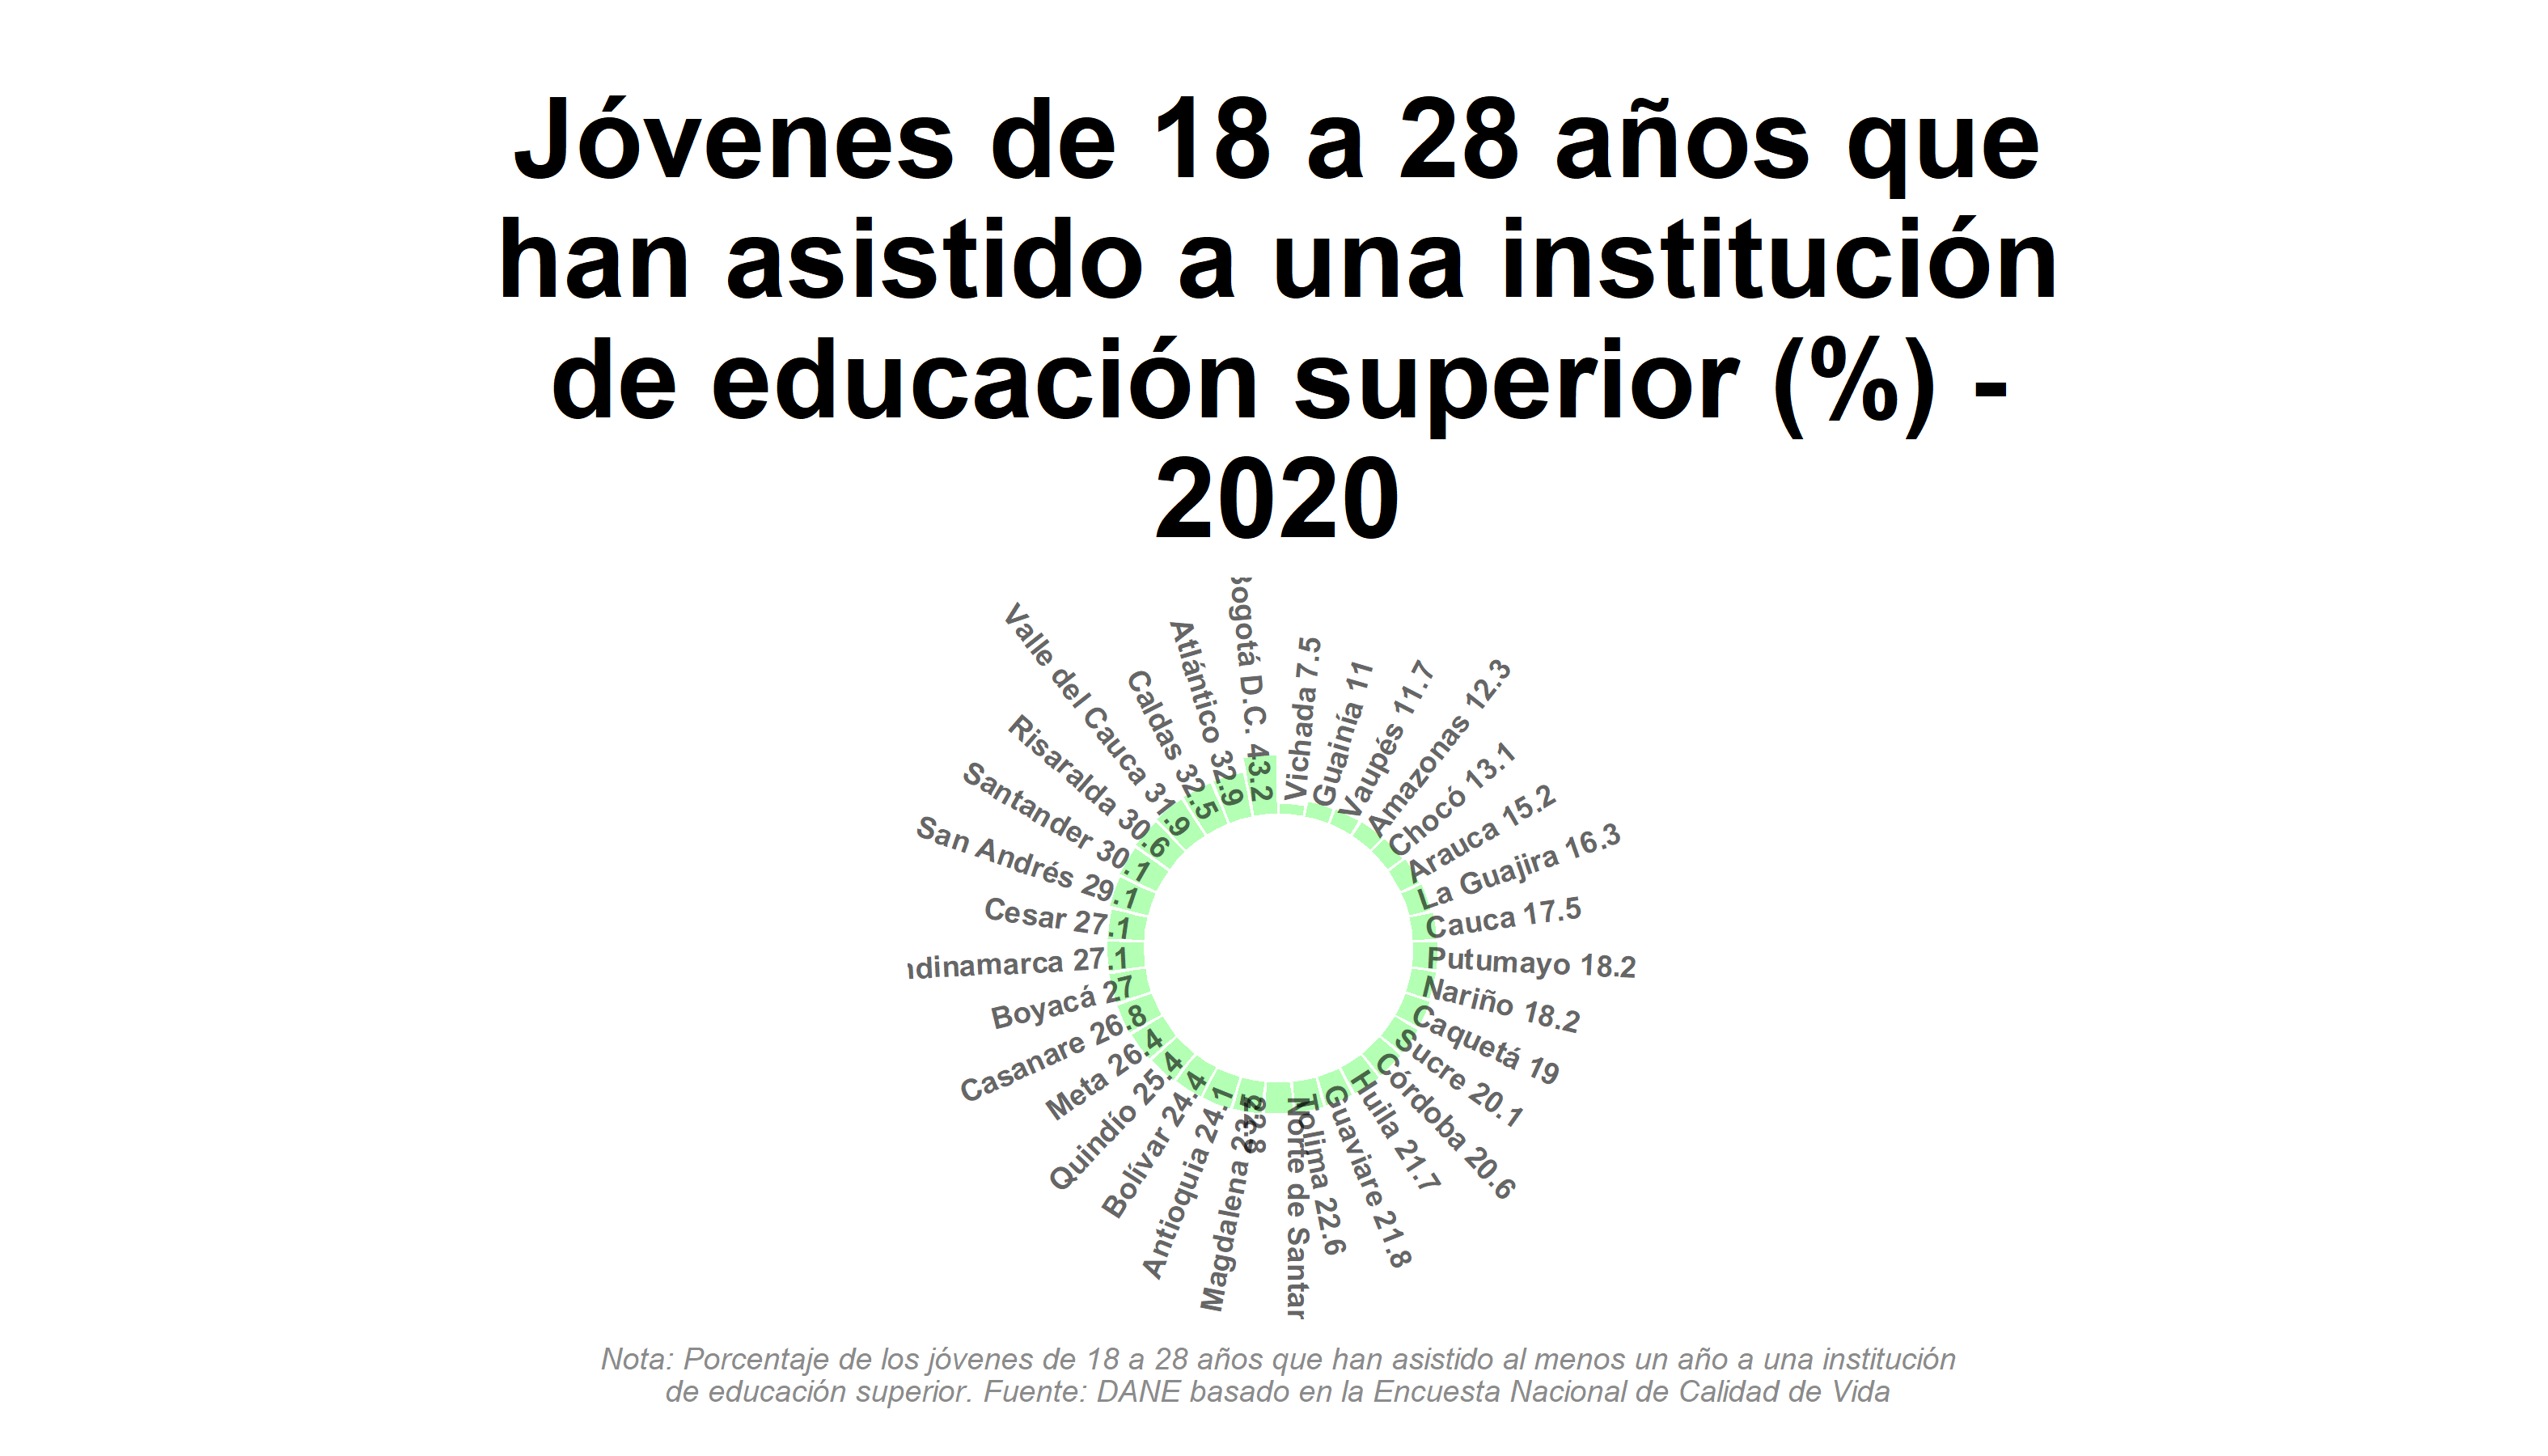
\includegraphics[width=\columnwidth]{img/var_127_static.png}
            \end{imagecolumn}
            \begin{textcolumn}
                \begin{itemize}
                    \item Existe una alta desigualdad en el acceso a la educación superior entre regiones
                    \item Mientras que en Bogotá el 43% de los jóvenes ha asistido a institutos de educación superior al menos por 1 año, en Vichada éste porcentaje es de 7%
                    \item Éstas diferencias no han cambiado mucho en el tiempo 
                \end{itemize}
            \end{textcolumn}

    \printcolumns
    \end{slide}
    
    %%%-- Fertilidad Adolescente
    \begin{slide}{14} 
            \begin{imagecolumn}
                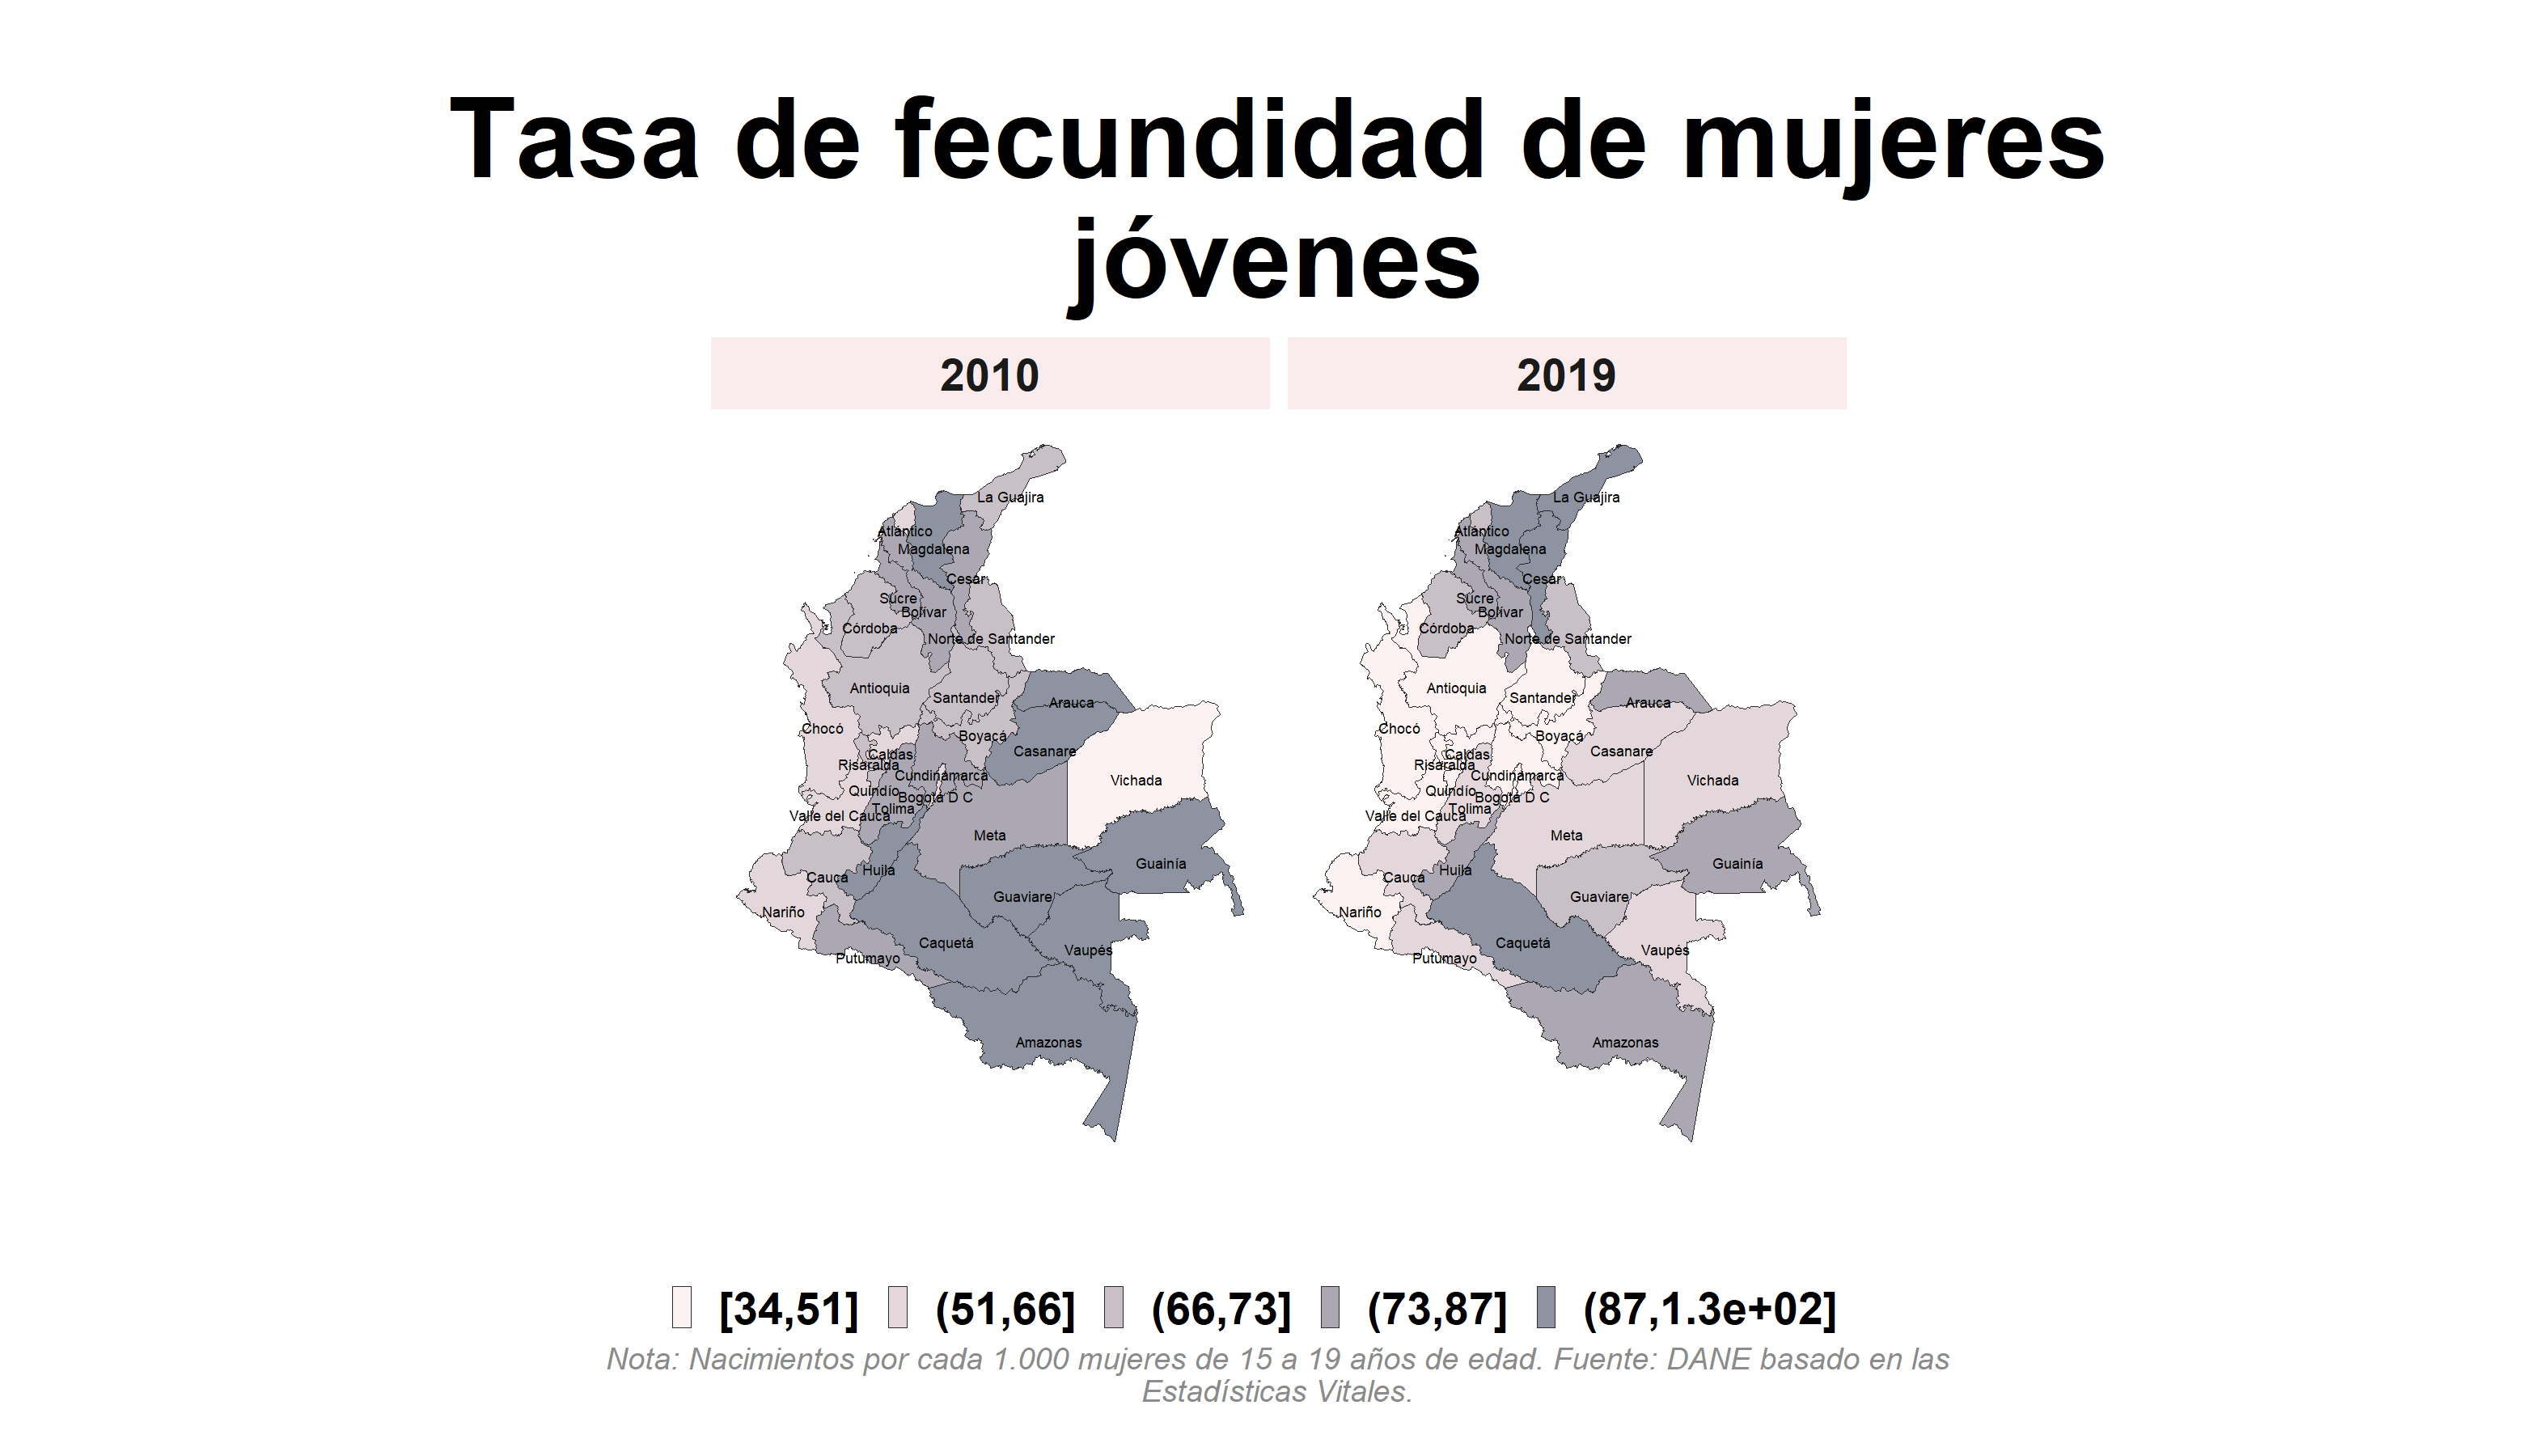
\includegraphics[width=\columnwidth]{img/var_282_map.png}
            \end{imagecolumn}
            \begin{textcolumn}
                \begin{itemize}
                    \item La tasa de fecundidad adolescente ha disminuido drásticamente en los últimos 10 años, pero hay gran heterogeneidad territorial.
                    \item En algunas zonas las tasas altas persisten (Caquetá), en otras zonas la fecundidad aumentó (La Guajira, Magdalena).
                \end{itemize}
            \end{textcolumn}

    \printcolumns
    \end{slide}
    
        %%%-- NINIS 
    \begin{slide}{14} 
                      \begin{imagecolumn}
                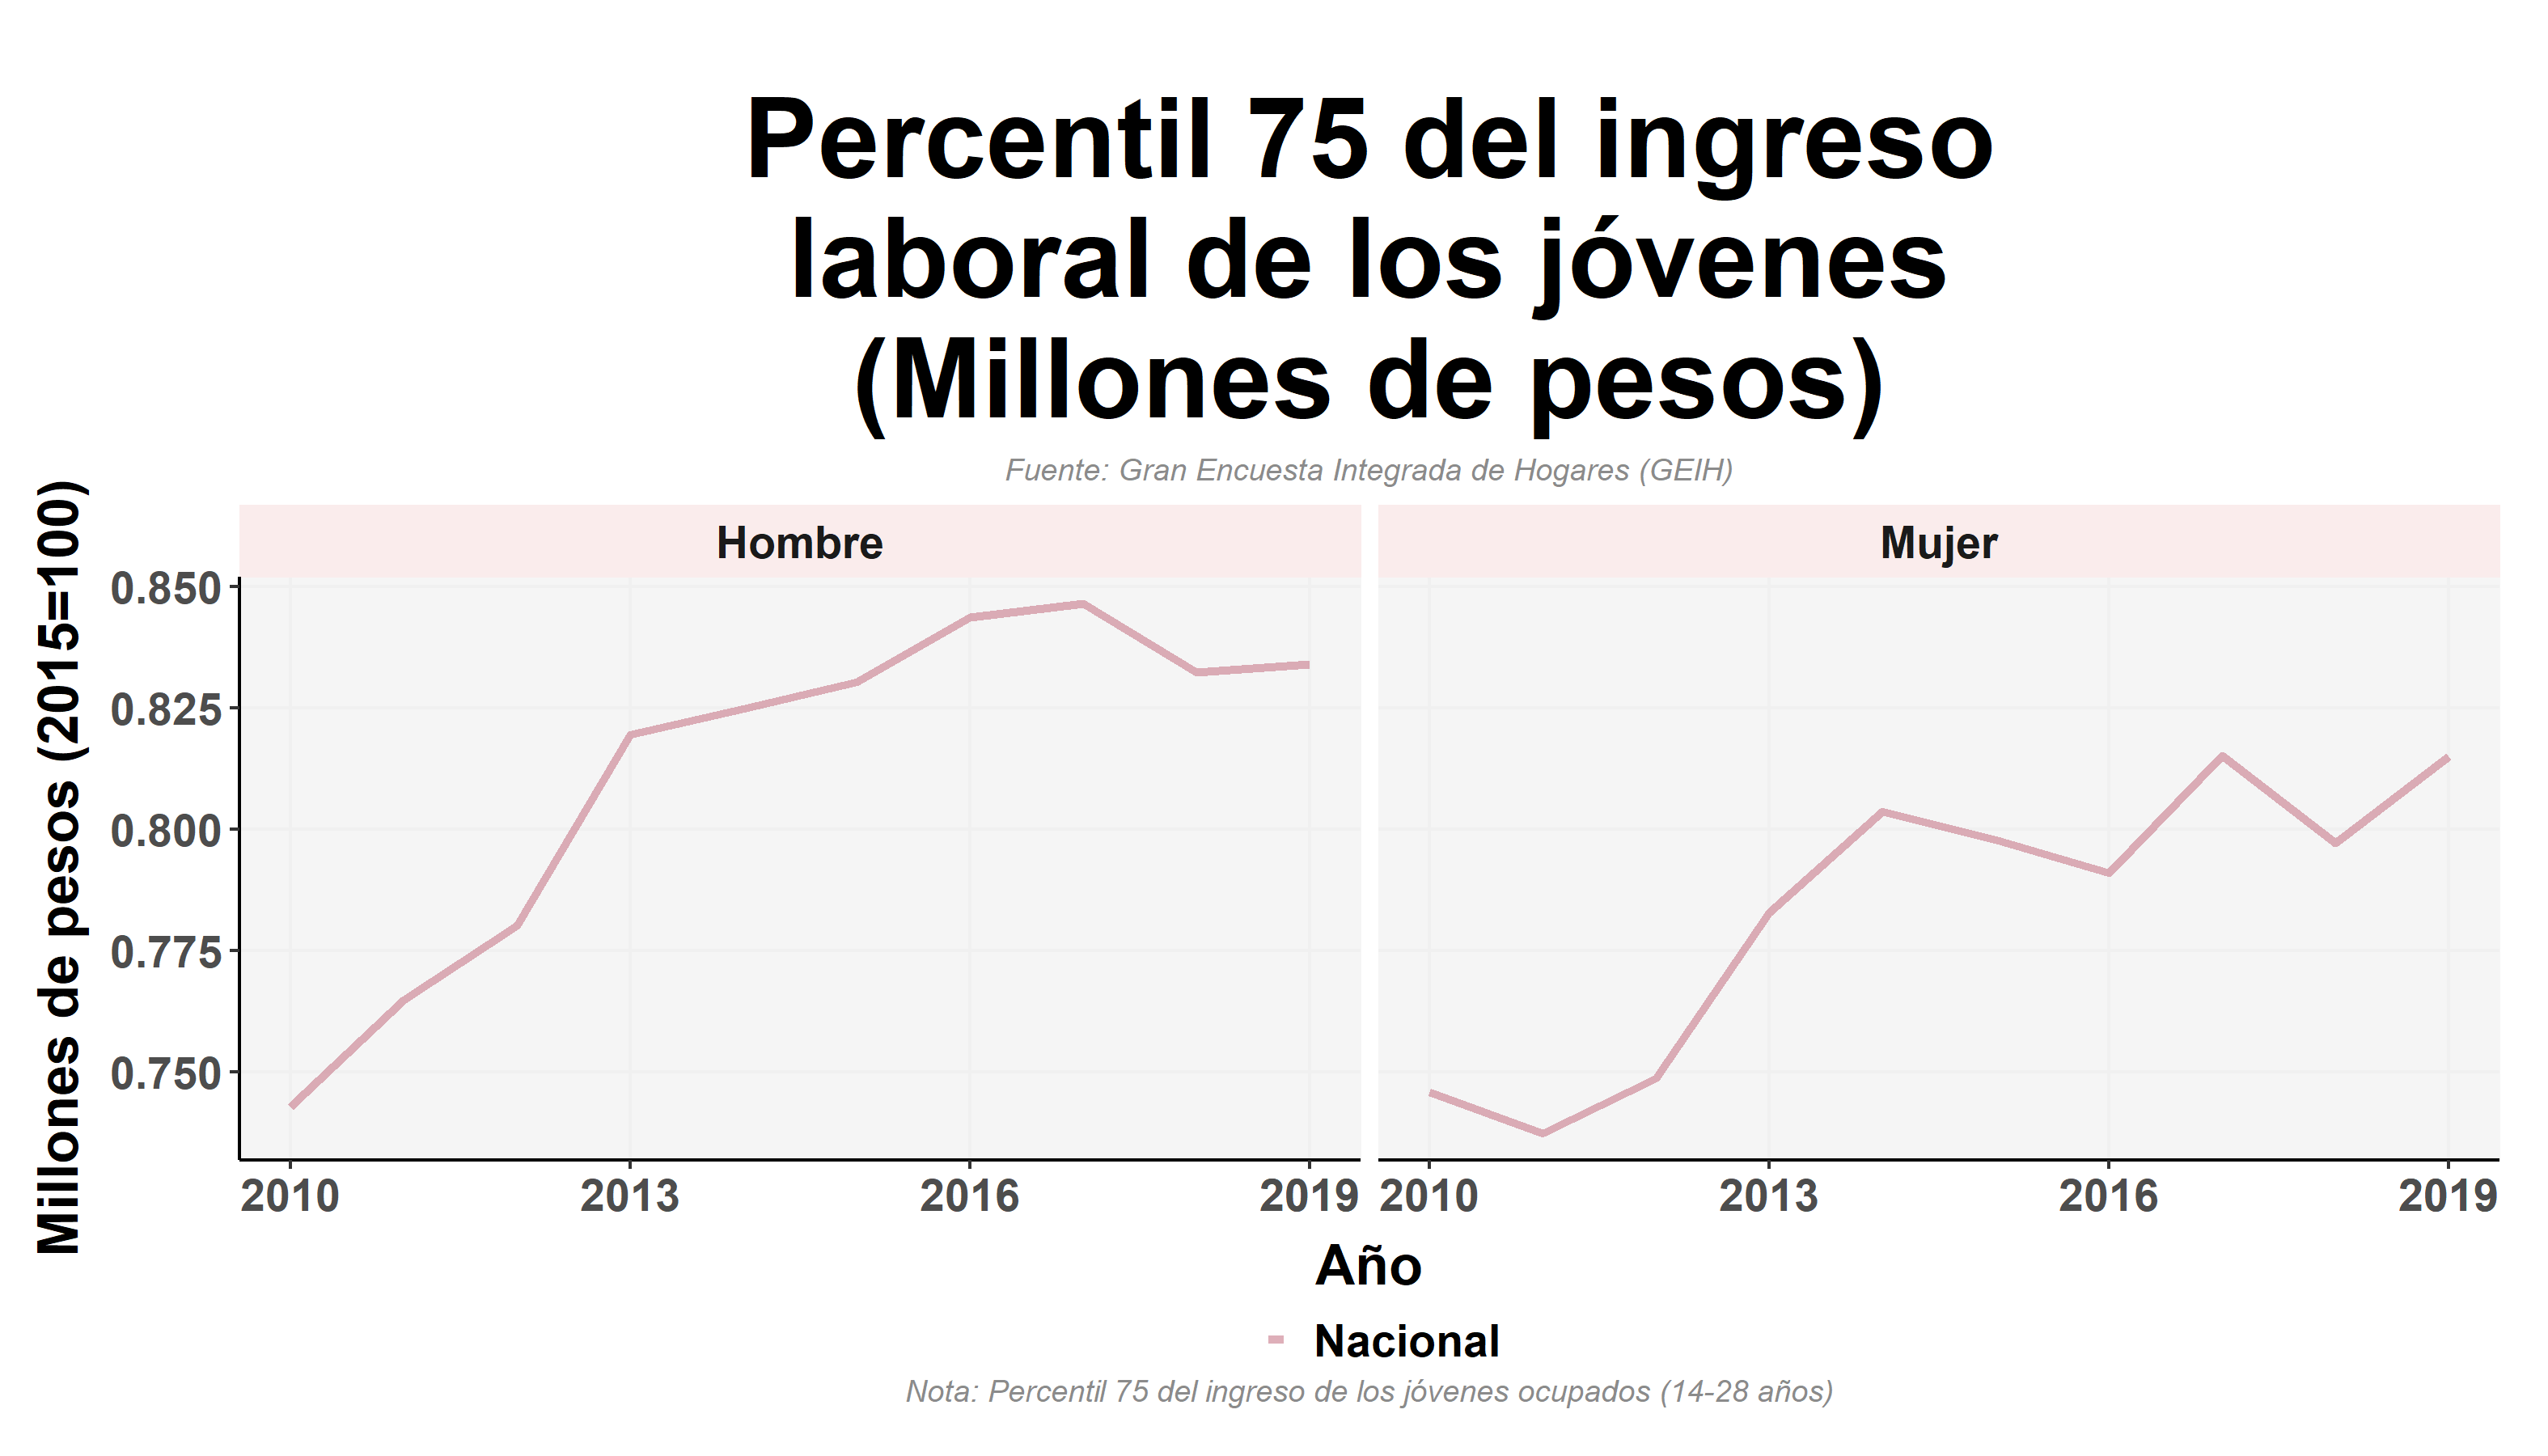
\includegraphics[width=\columnwidth]{img/var_41_trend.png}
            \end{imagecolumn}
            \begin{textcolumn}
                \begin{itemize}
                    \item La tasa de mujeres jóvenes que ni estudian, ni trabajan es casi el doble que la de los hombres jóvenes
                    \item Esta tendencia se agudizó con la pandemia.
                \end{itemize}
            \end{textcolumn}

    \printcolumns
    \end{slide}
    
    %%%-- Desempleo Juvenil
    \begin{slide}{14} 
            \begin{imagecolumn}
                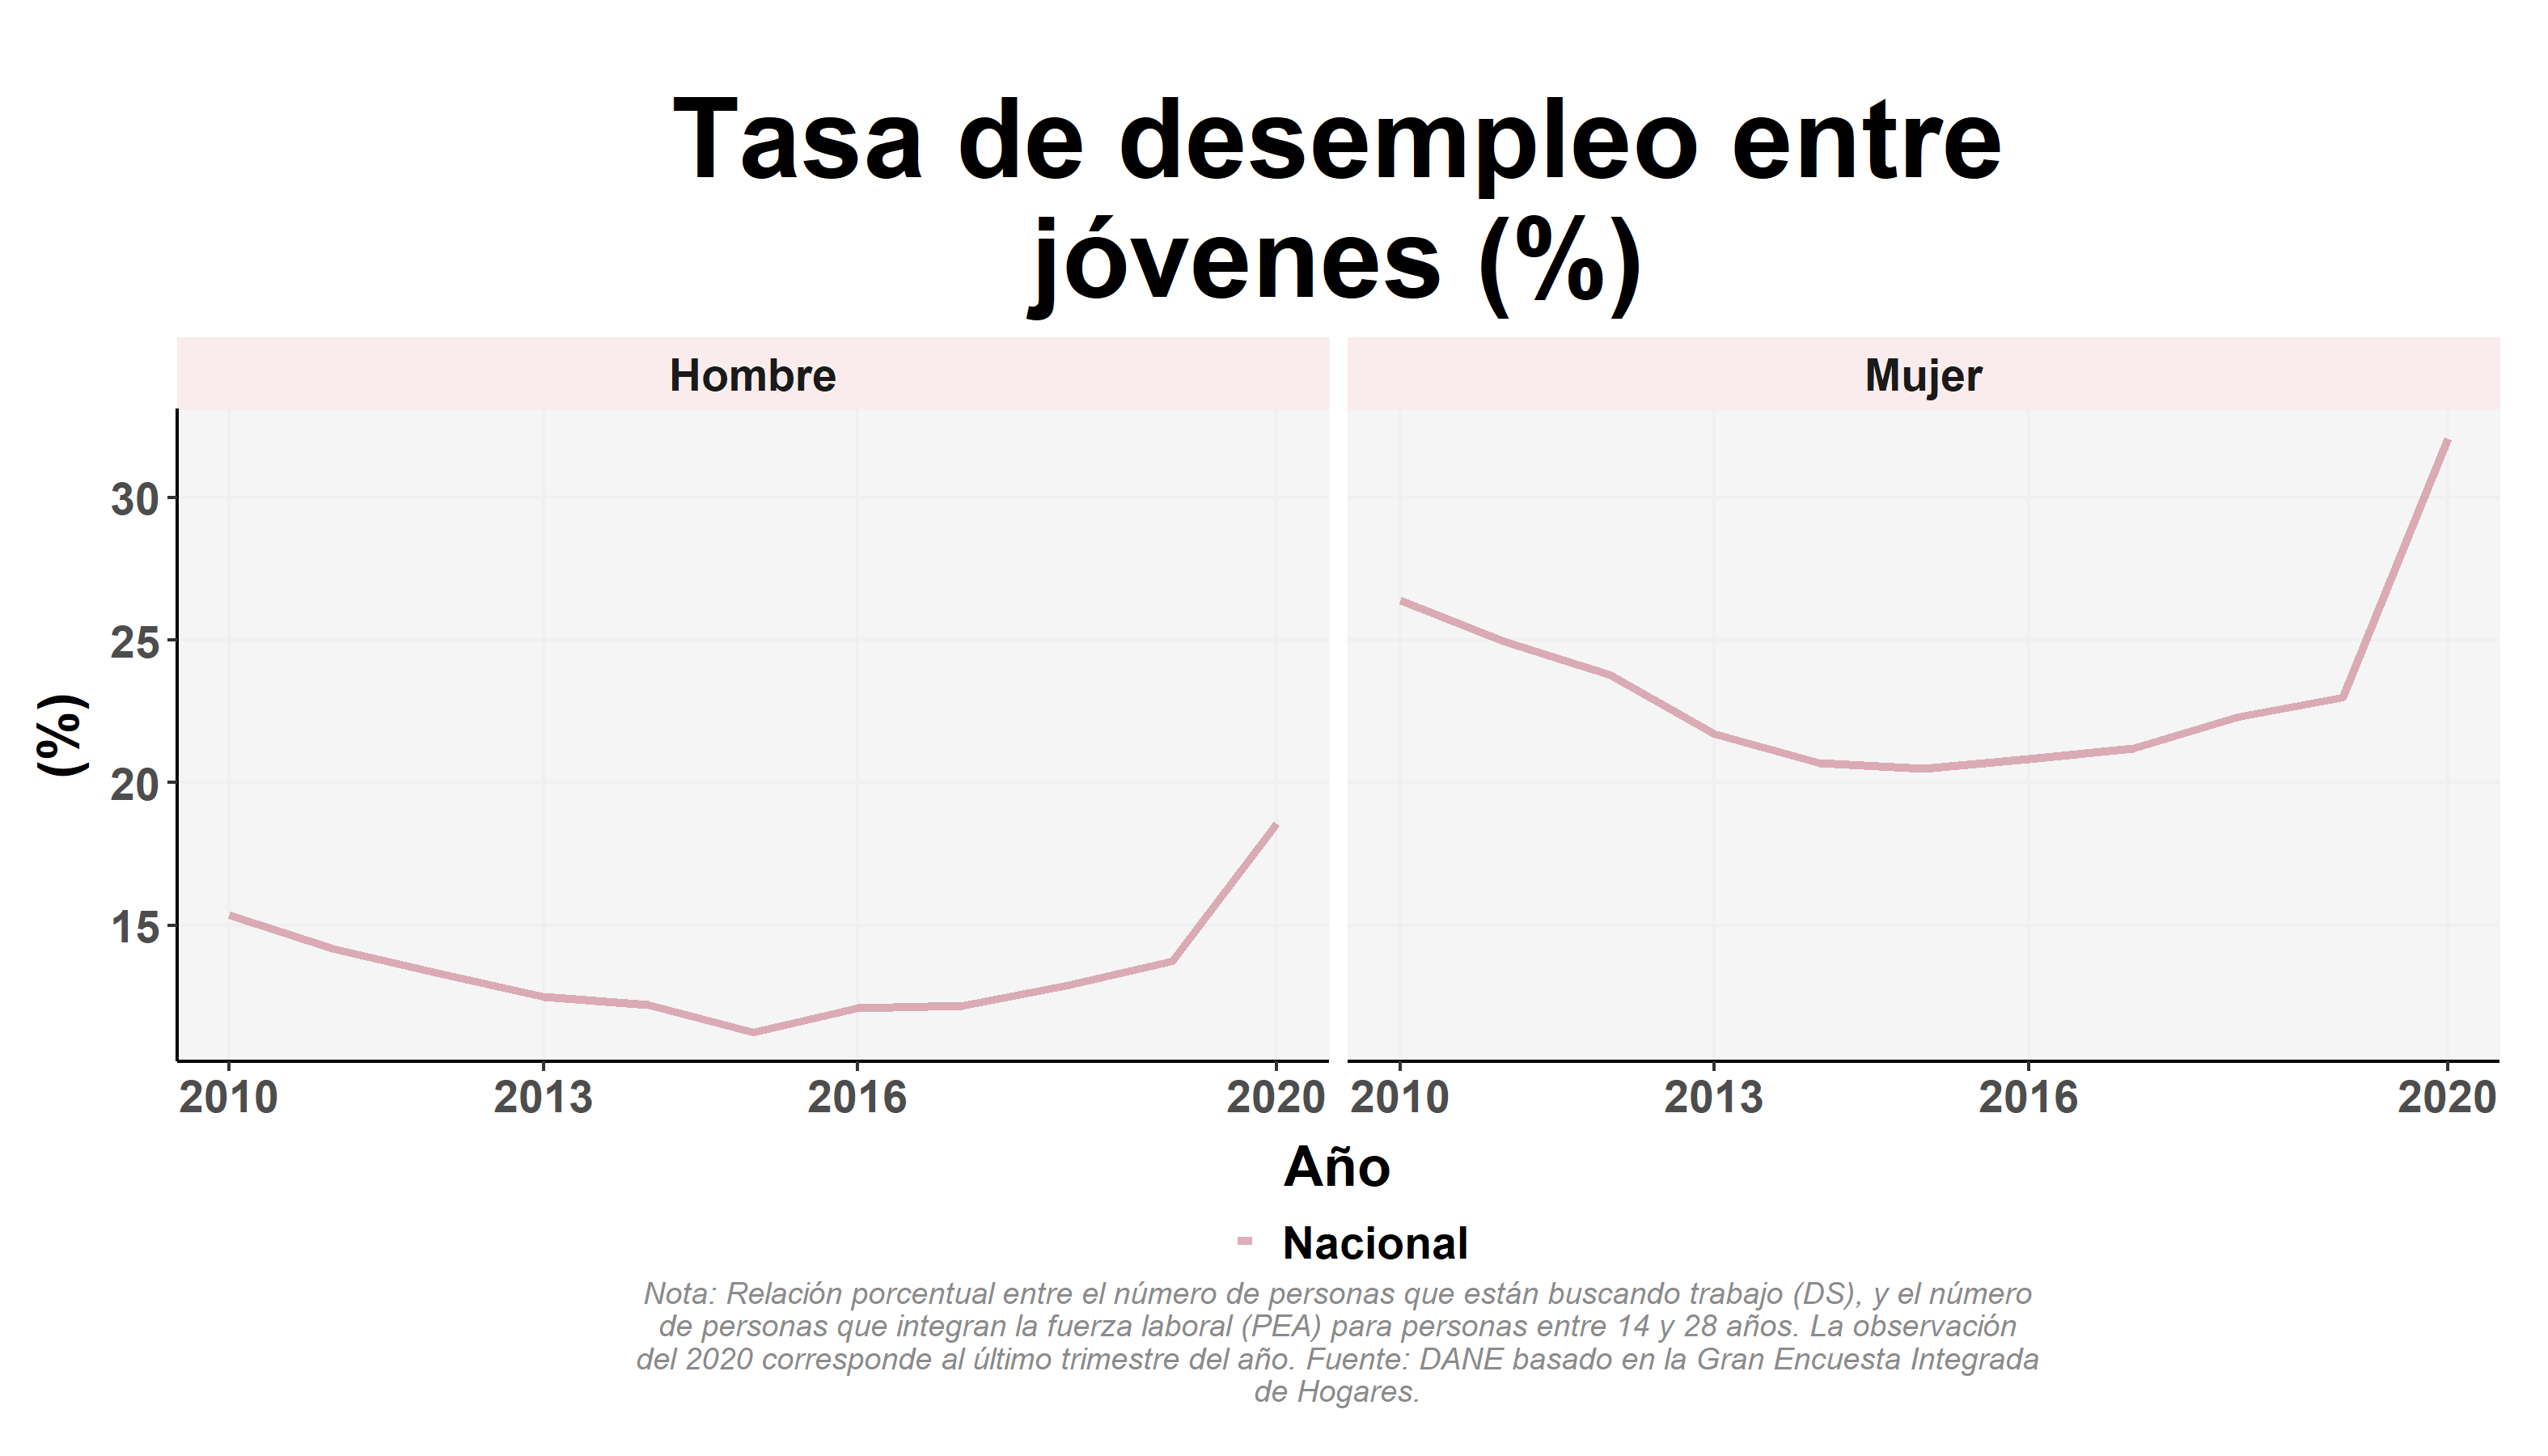
\includegraphics[width=\columnwidth]{img/var_55_trend.png}
            \end{imagecolumn}
            \begin{textcolumn}
                \begin{itemize}
                    \item La tasa de desempleo entre jóvenes tiene una tendencia similar.
                    \item Grandes brechas de género que se agudizaron con la pandemia
                \end{itemize}
            \end{textcolumn}
    \printcolumns
    \end{slide}
    
        %%%-- Informalidad
    \begin{slide}{14} 
            \begin{imagecolumn}
                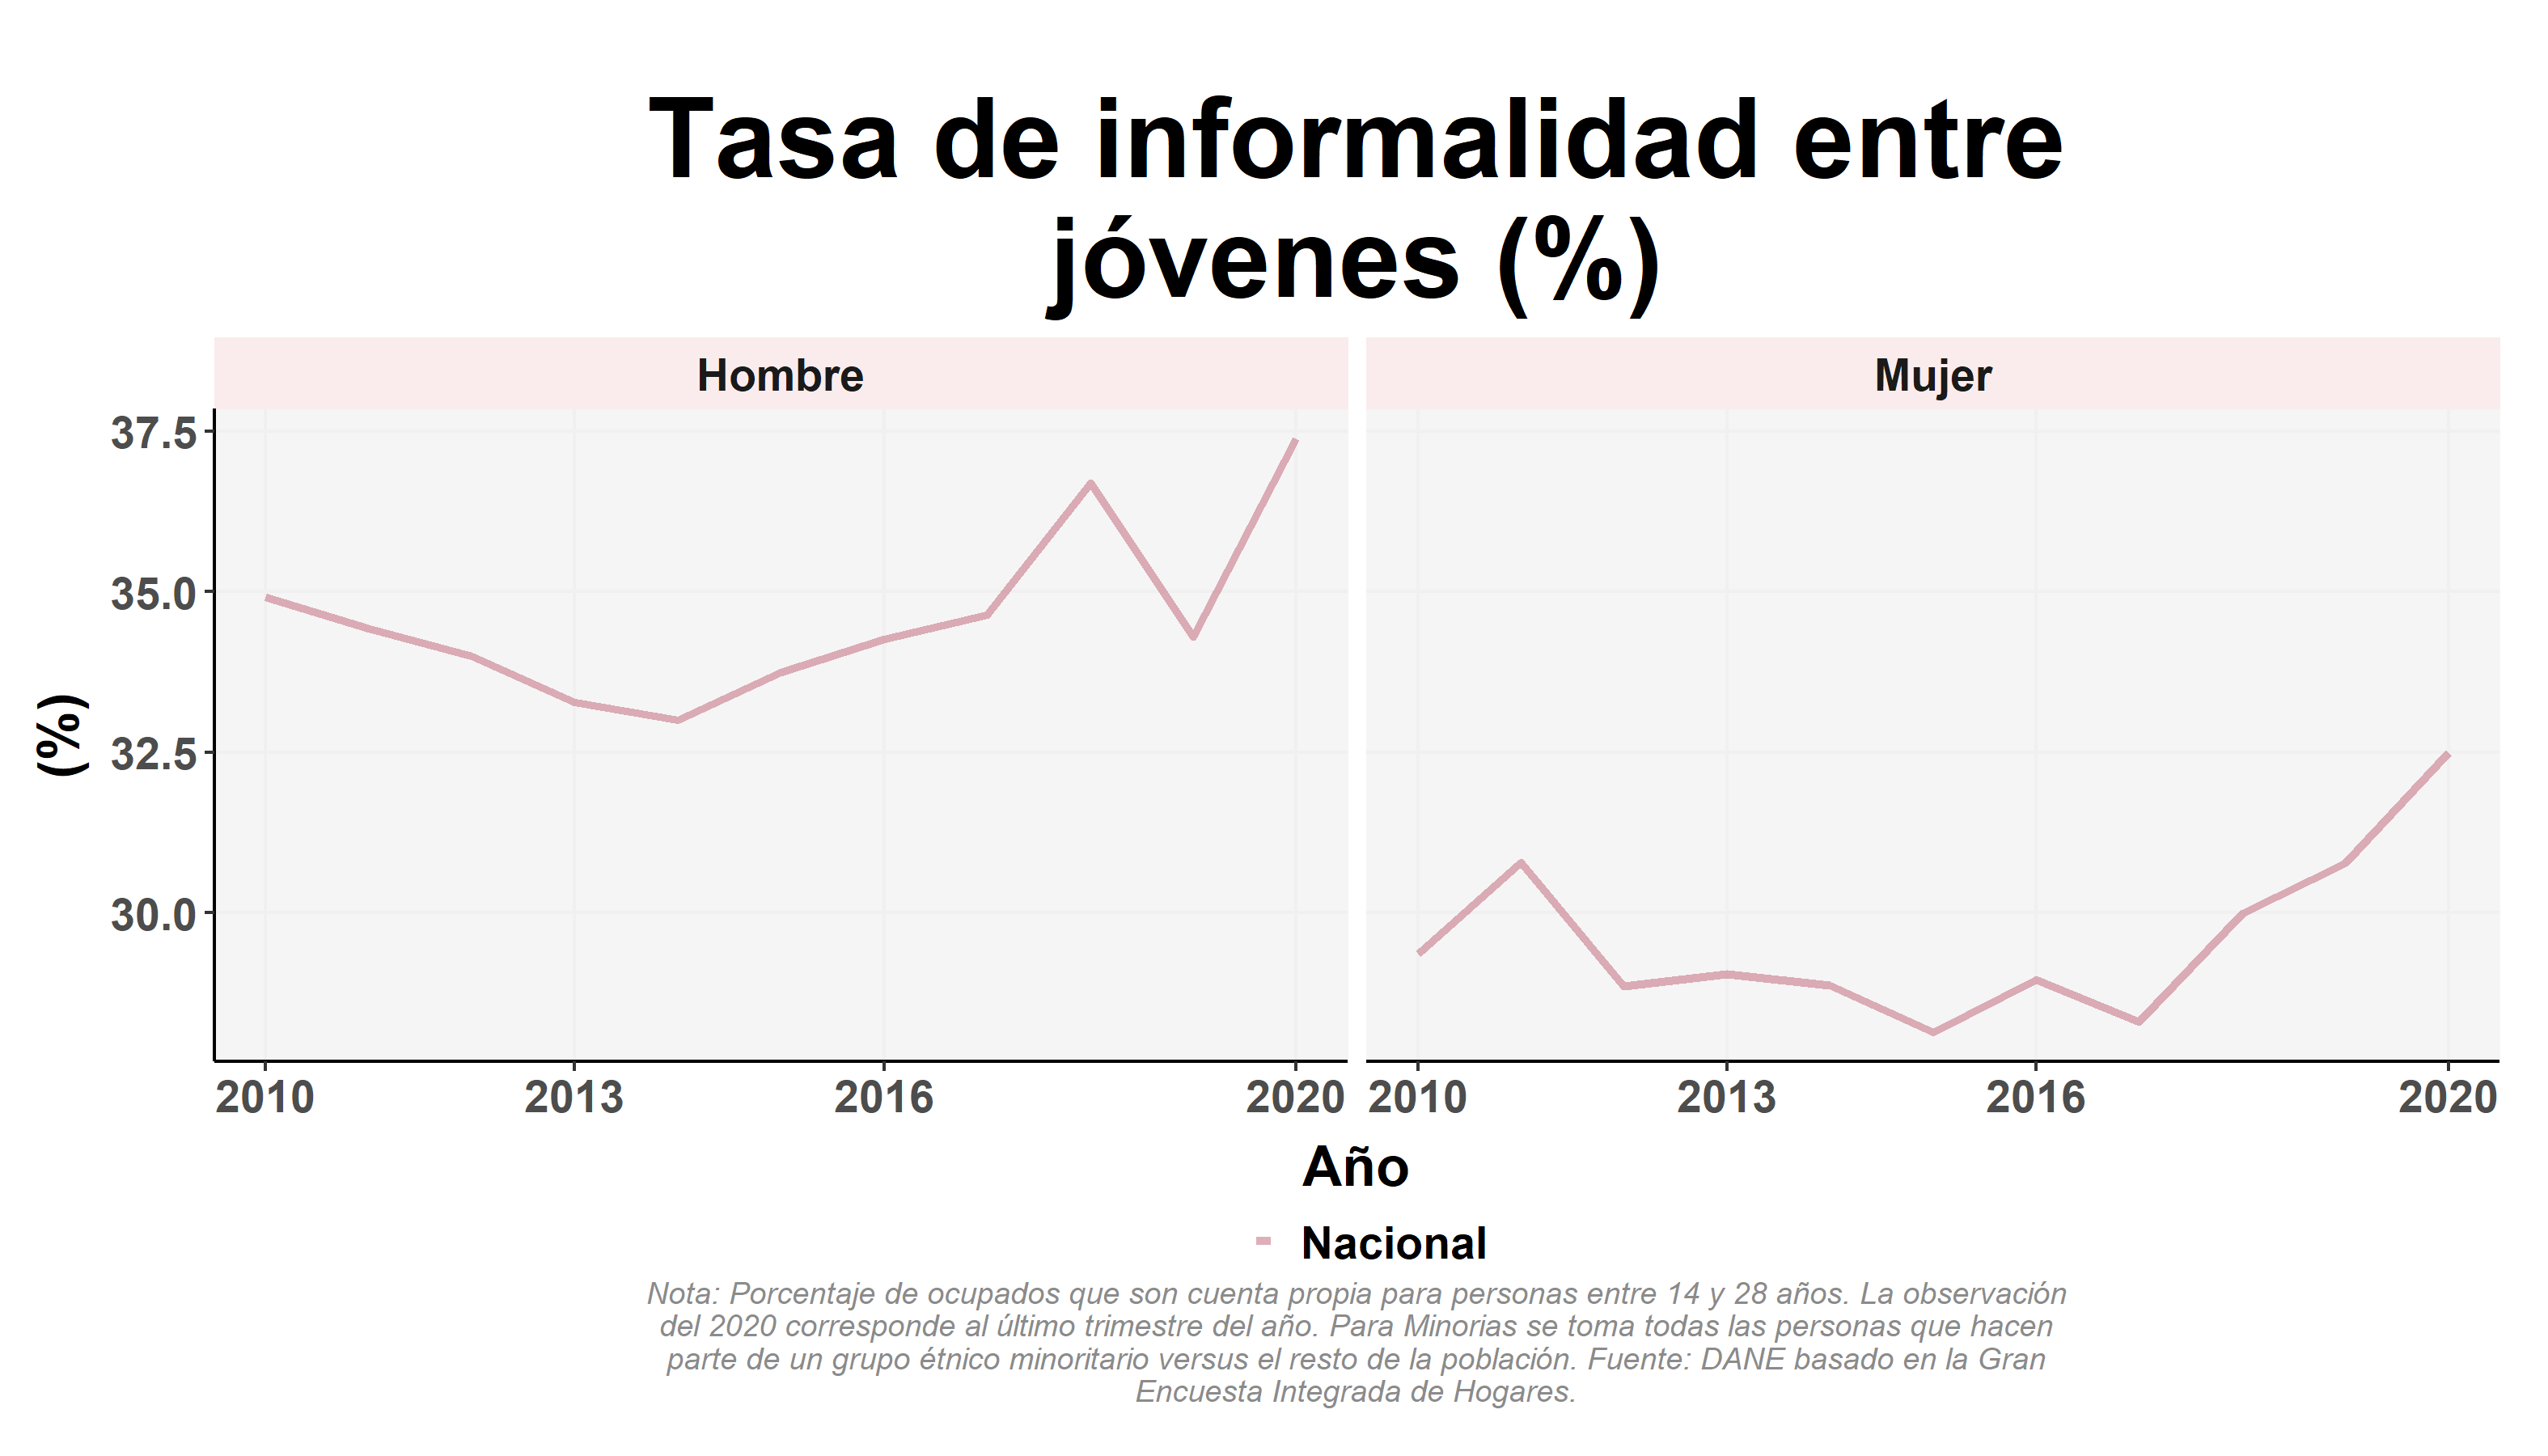
\includegraphics[width=\columnwidth]{img/var_75_trend.png}
            \end{imagecolumn}
            \begin{textcolumn}
                \begin{itemize}
                    \item La informalidad joven es más alta entre hombres que entre mujeres. 
                    \item Pero ha aumentado más entre mujeres jóvenes en los últimos años
                \end{itemize}
            \end{textcolumn}
    \printcolumns
    \end{slide}
    
      %%% ----------------------------
    %%% Adultez
    %%% ----------------------------
    \subsection{Adultez}

            %%%-- Desempleo por ciudad
    \begin{slide}{15} 
            \begin{imagecolumn}
                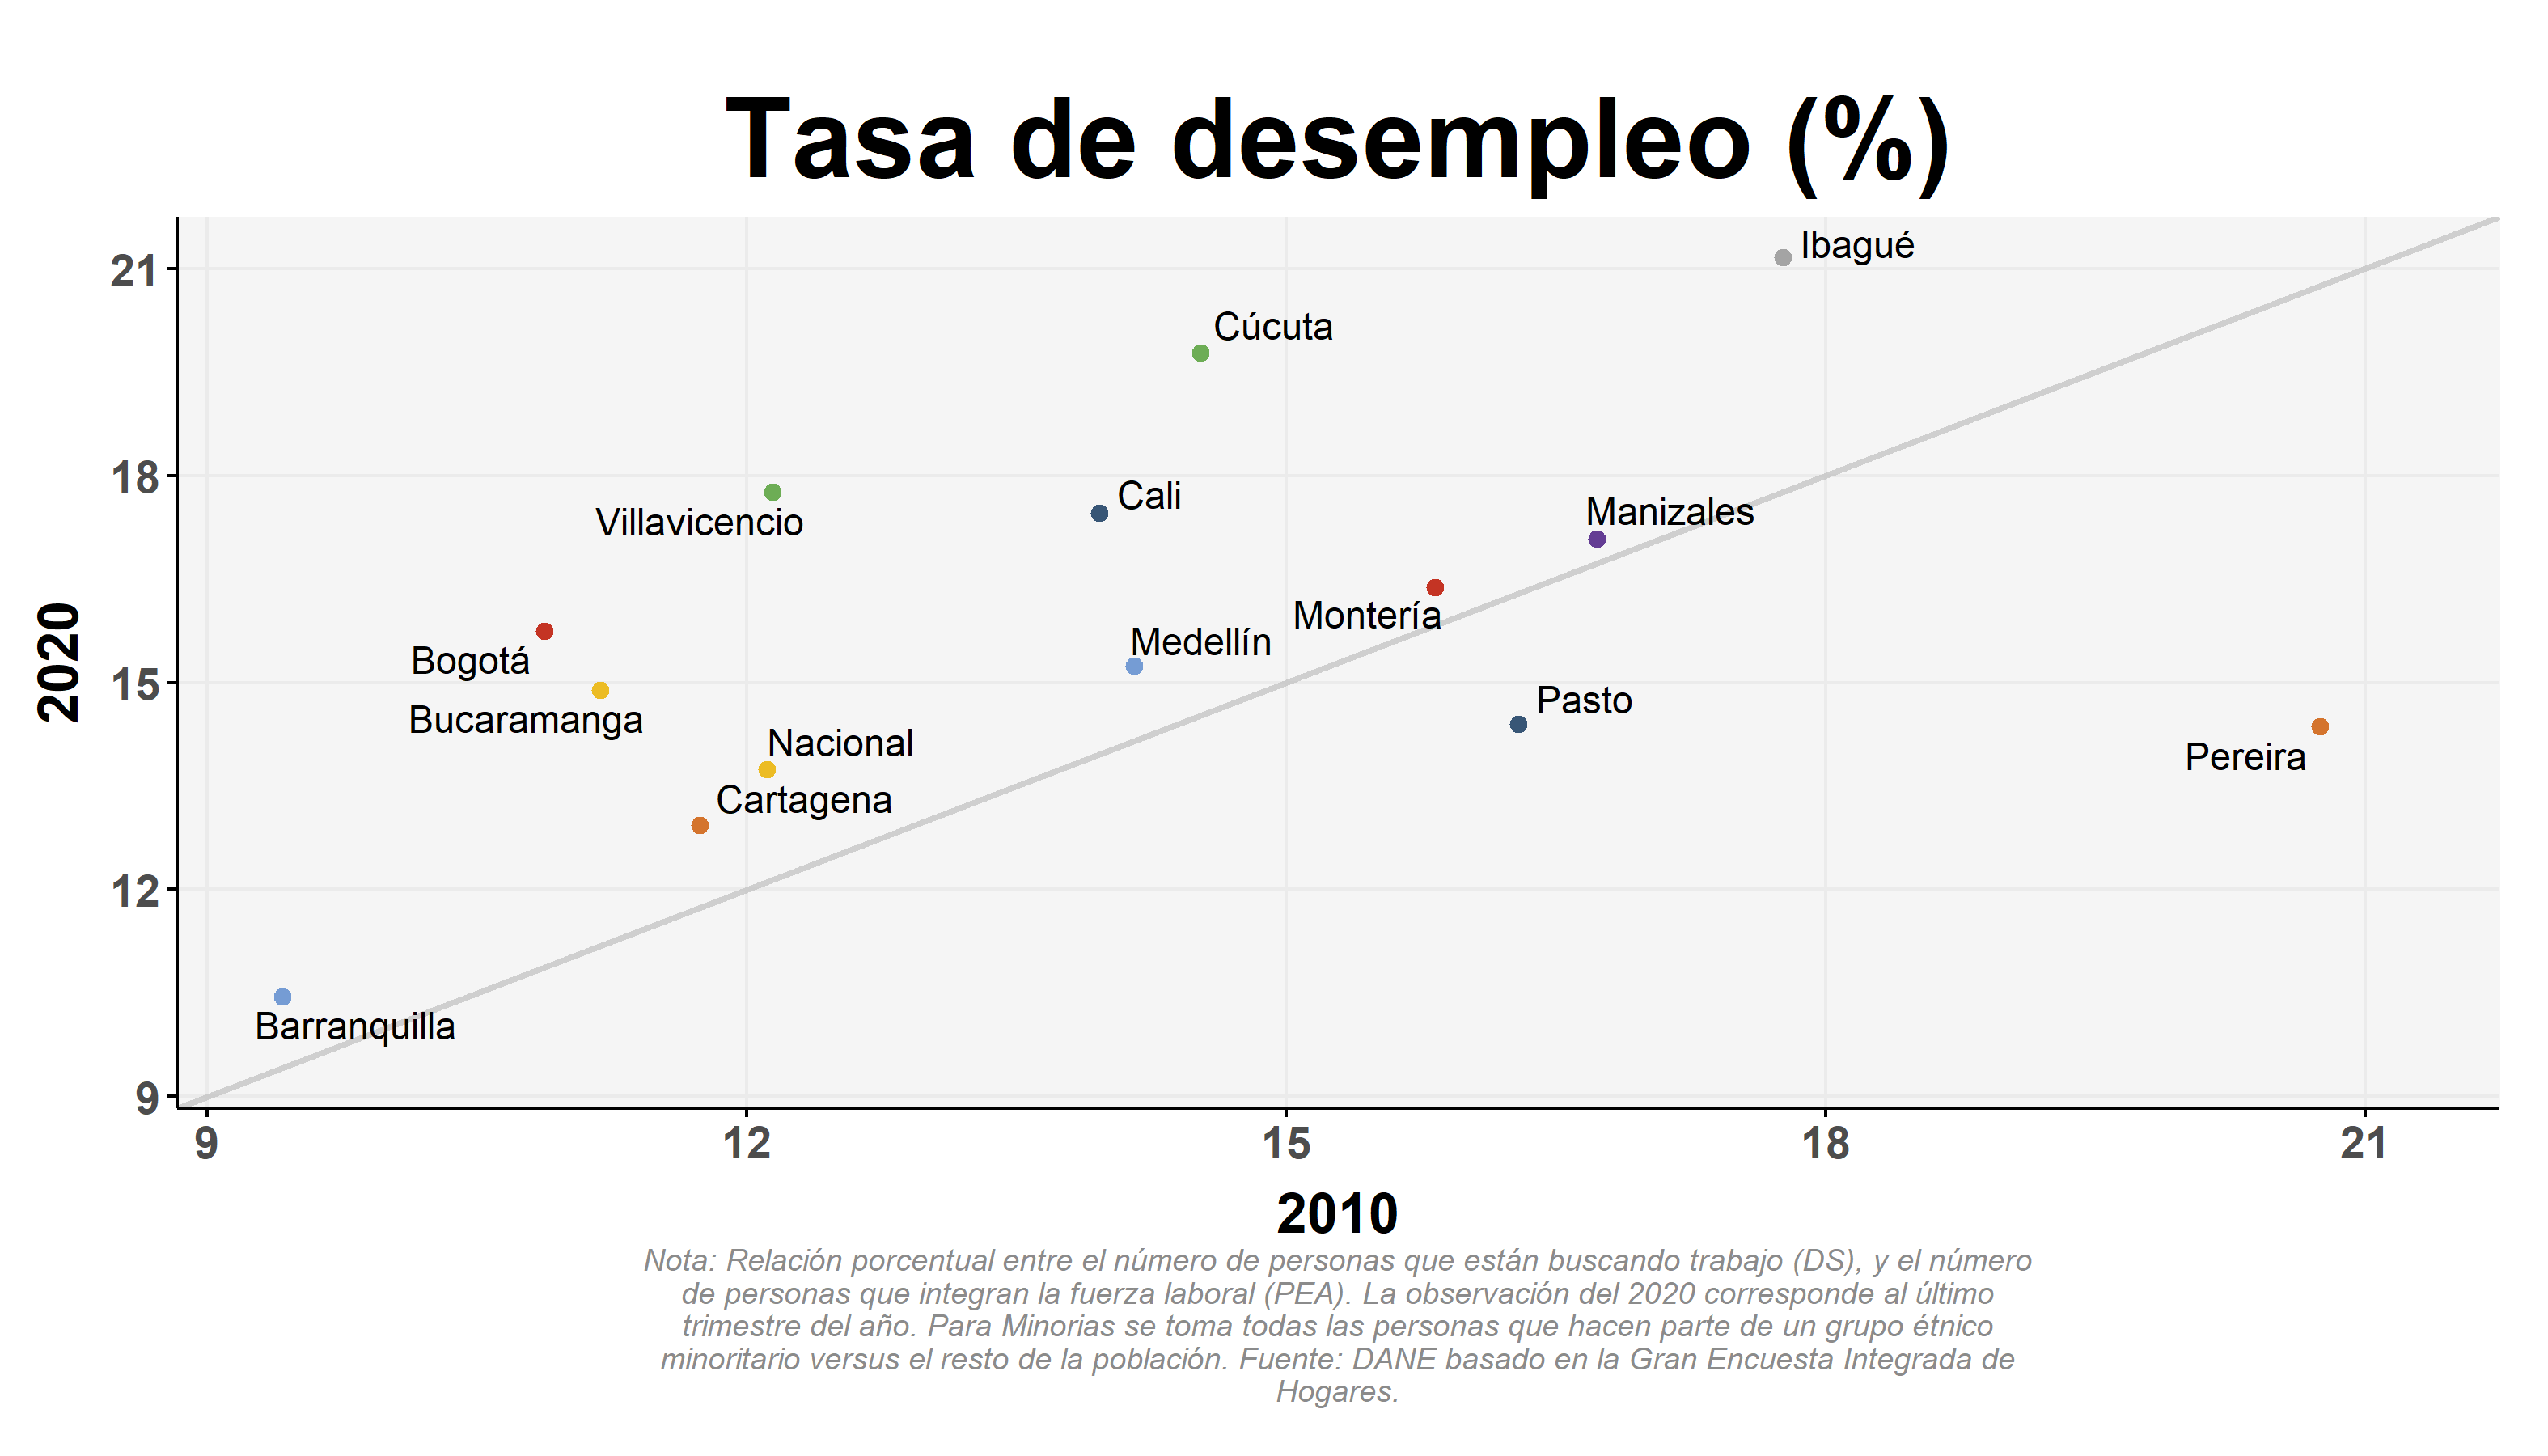
\includegraphics[width=\columnwidth]{img/var_45_scatter_time.png}
            \end{imagecolumn}
            \begin{textcolumn}
                \begin{itemize}
                    \item Un incremento en el desempleo generalizado debido a la pandemia
                    \item Con algunas ciudades donde se ha agudizado en mayor magnitud
                \end{itemize}
            \end{textcolumn}
    \printcolumns
    \end{slide}
    
        %%%-- Desempleo por genero
        \begin{slide}{15} 
            \begin{imagecolumn}
                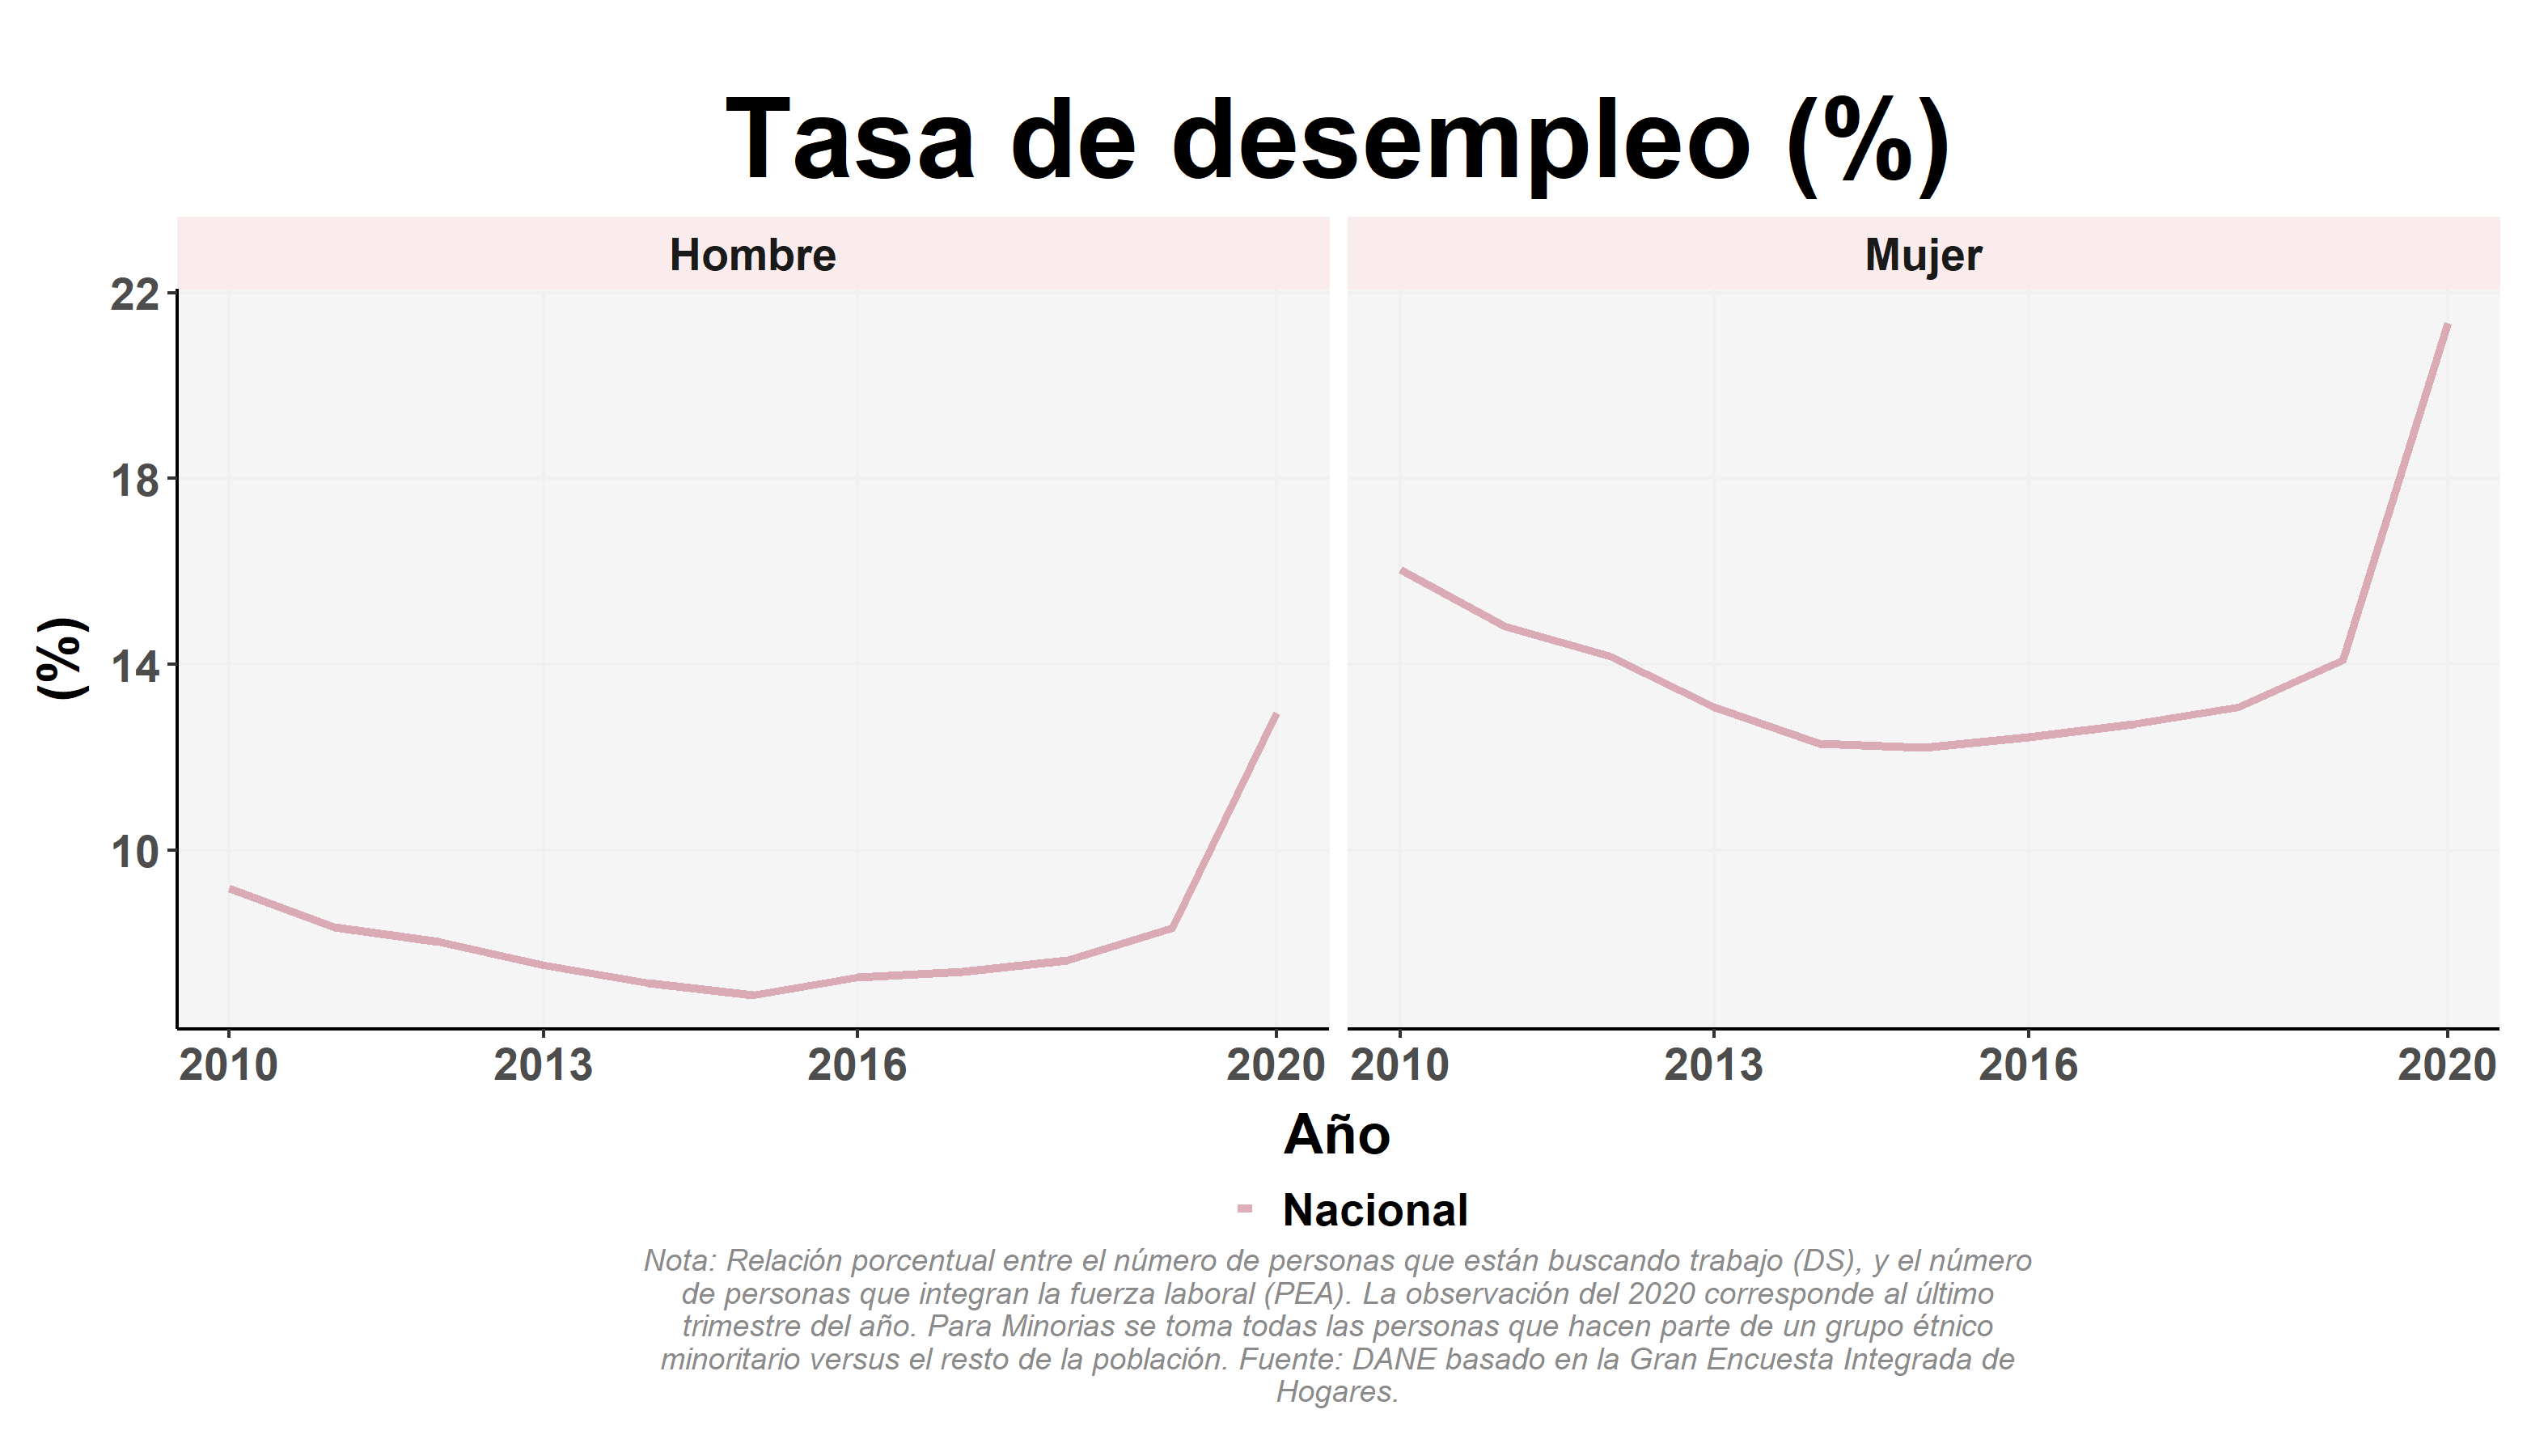
\includegraphics[width=\columnwidth]{img/var_49_trend.png}
            \end{imagecolumn}
            \begin{textcolumn}
                \begin{itemize}
                    \item El desempleo entre las mujeres está rezagado 10 años con respecto al de los hombres
                    \item La pandemia aumentó el desempleo de mujeres a un nivel sin precedentes.
                \end{itemize}
            \end{textcolumn}
    \printcolumns
    \end{slide}
    
        %%%-- Desempleo por etnia
        \begin{slide}{15} 
            \begin{imagecolumn}
                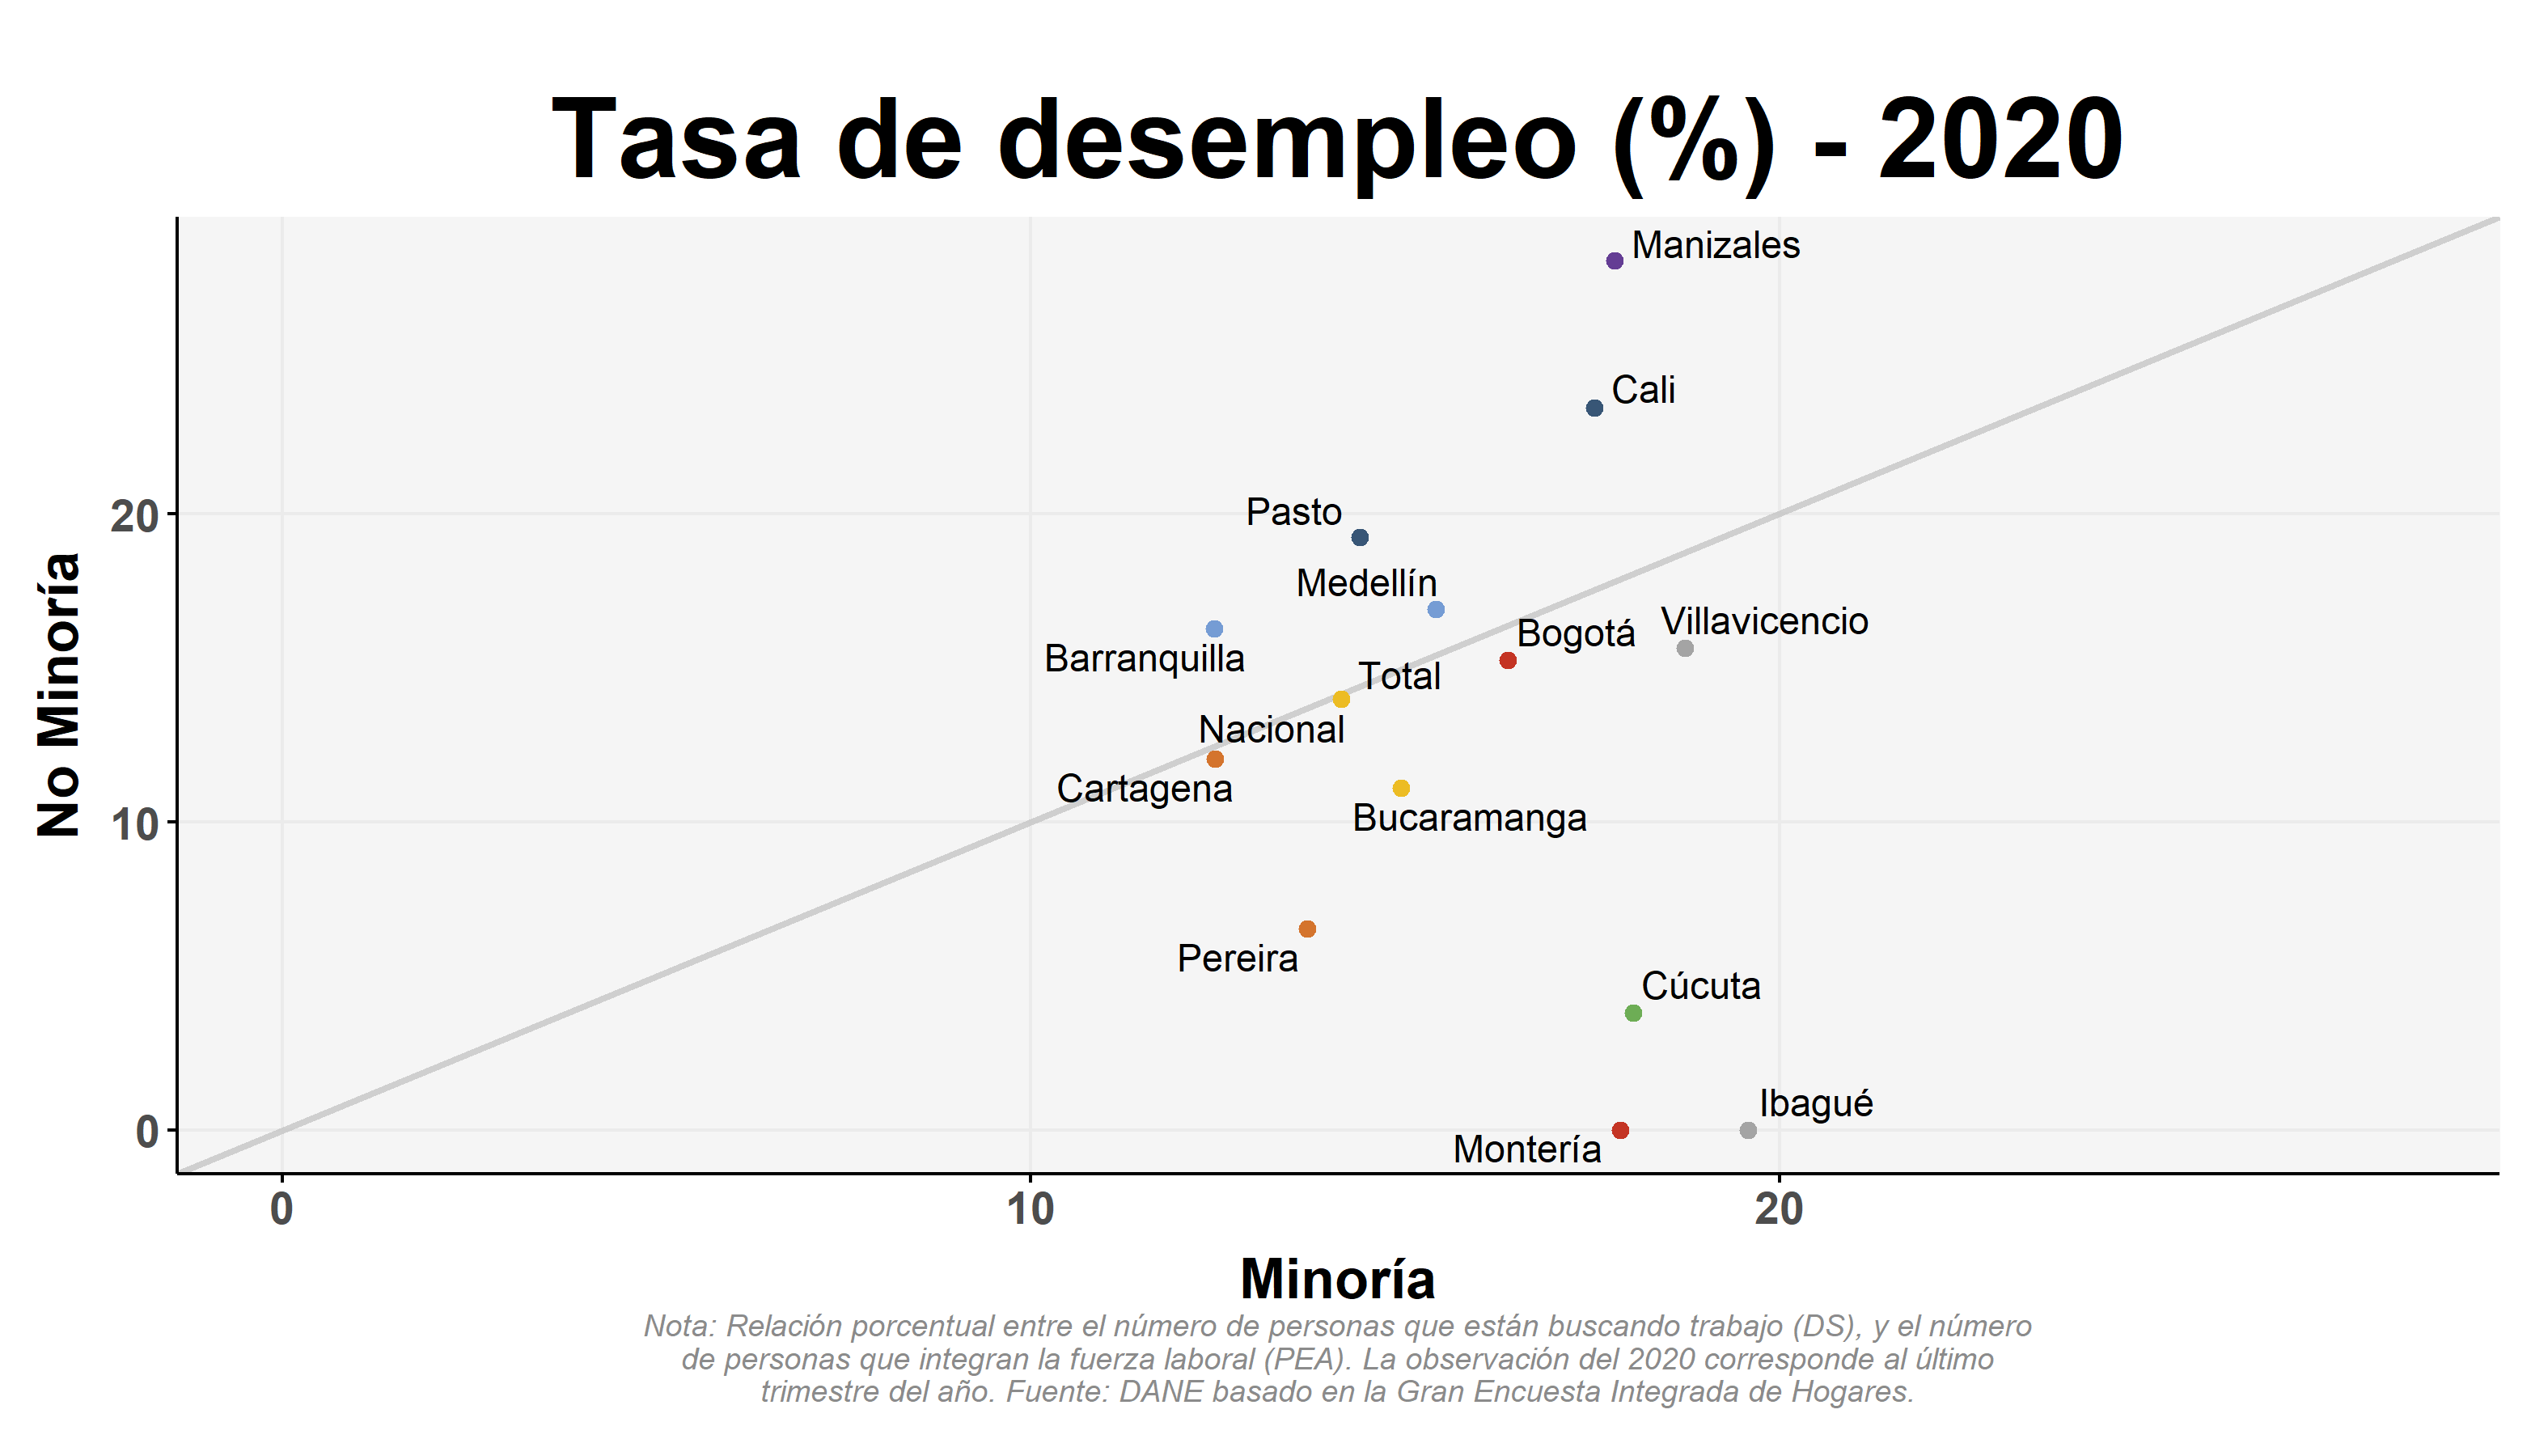
\includegraphics[width=\columnwidth]{img/var_43_scatter.png}
            \end{imagecolumn}
            \begin{textcolumn}
                \begin{itemize}
                    \item Las oportunidades de empleo para las minorias varían de acuerdo a la región. 
                    \item En ciudades como Montería, Ibagué y Cúcuta, las tasas de desempleo de las minorías son más altas que las del resto.
                \end{itemize}
            \end{textcolumn}
    \printcolumns
    \end{slide}    
    
        %%%-- Informalidad 
        \begin{slide}{15} 
            \begin{imagecolumn}
                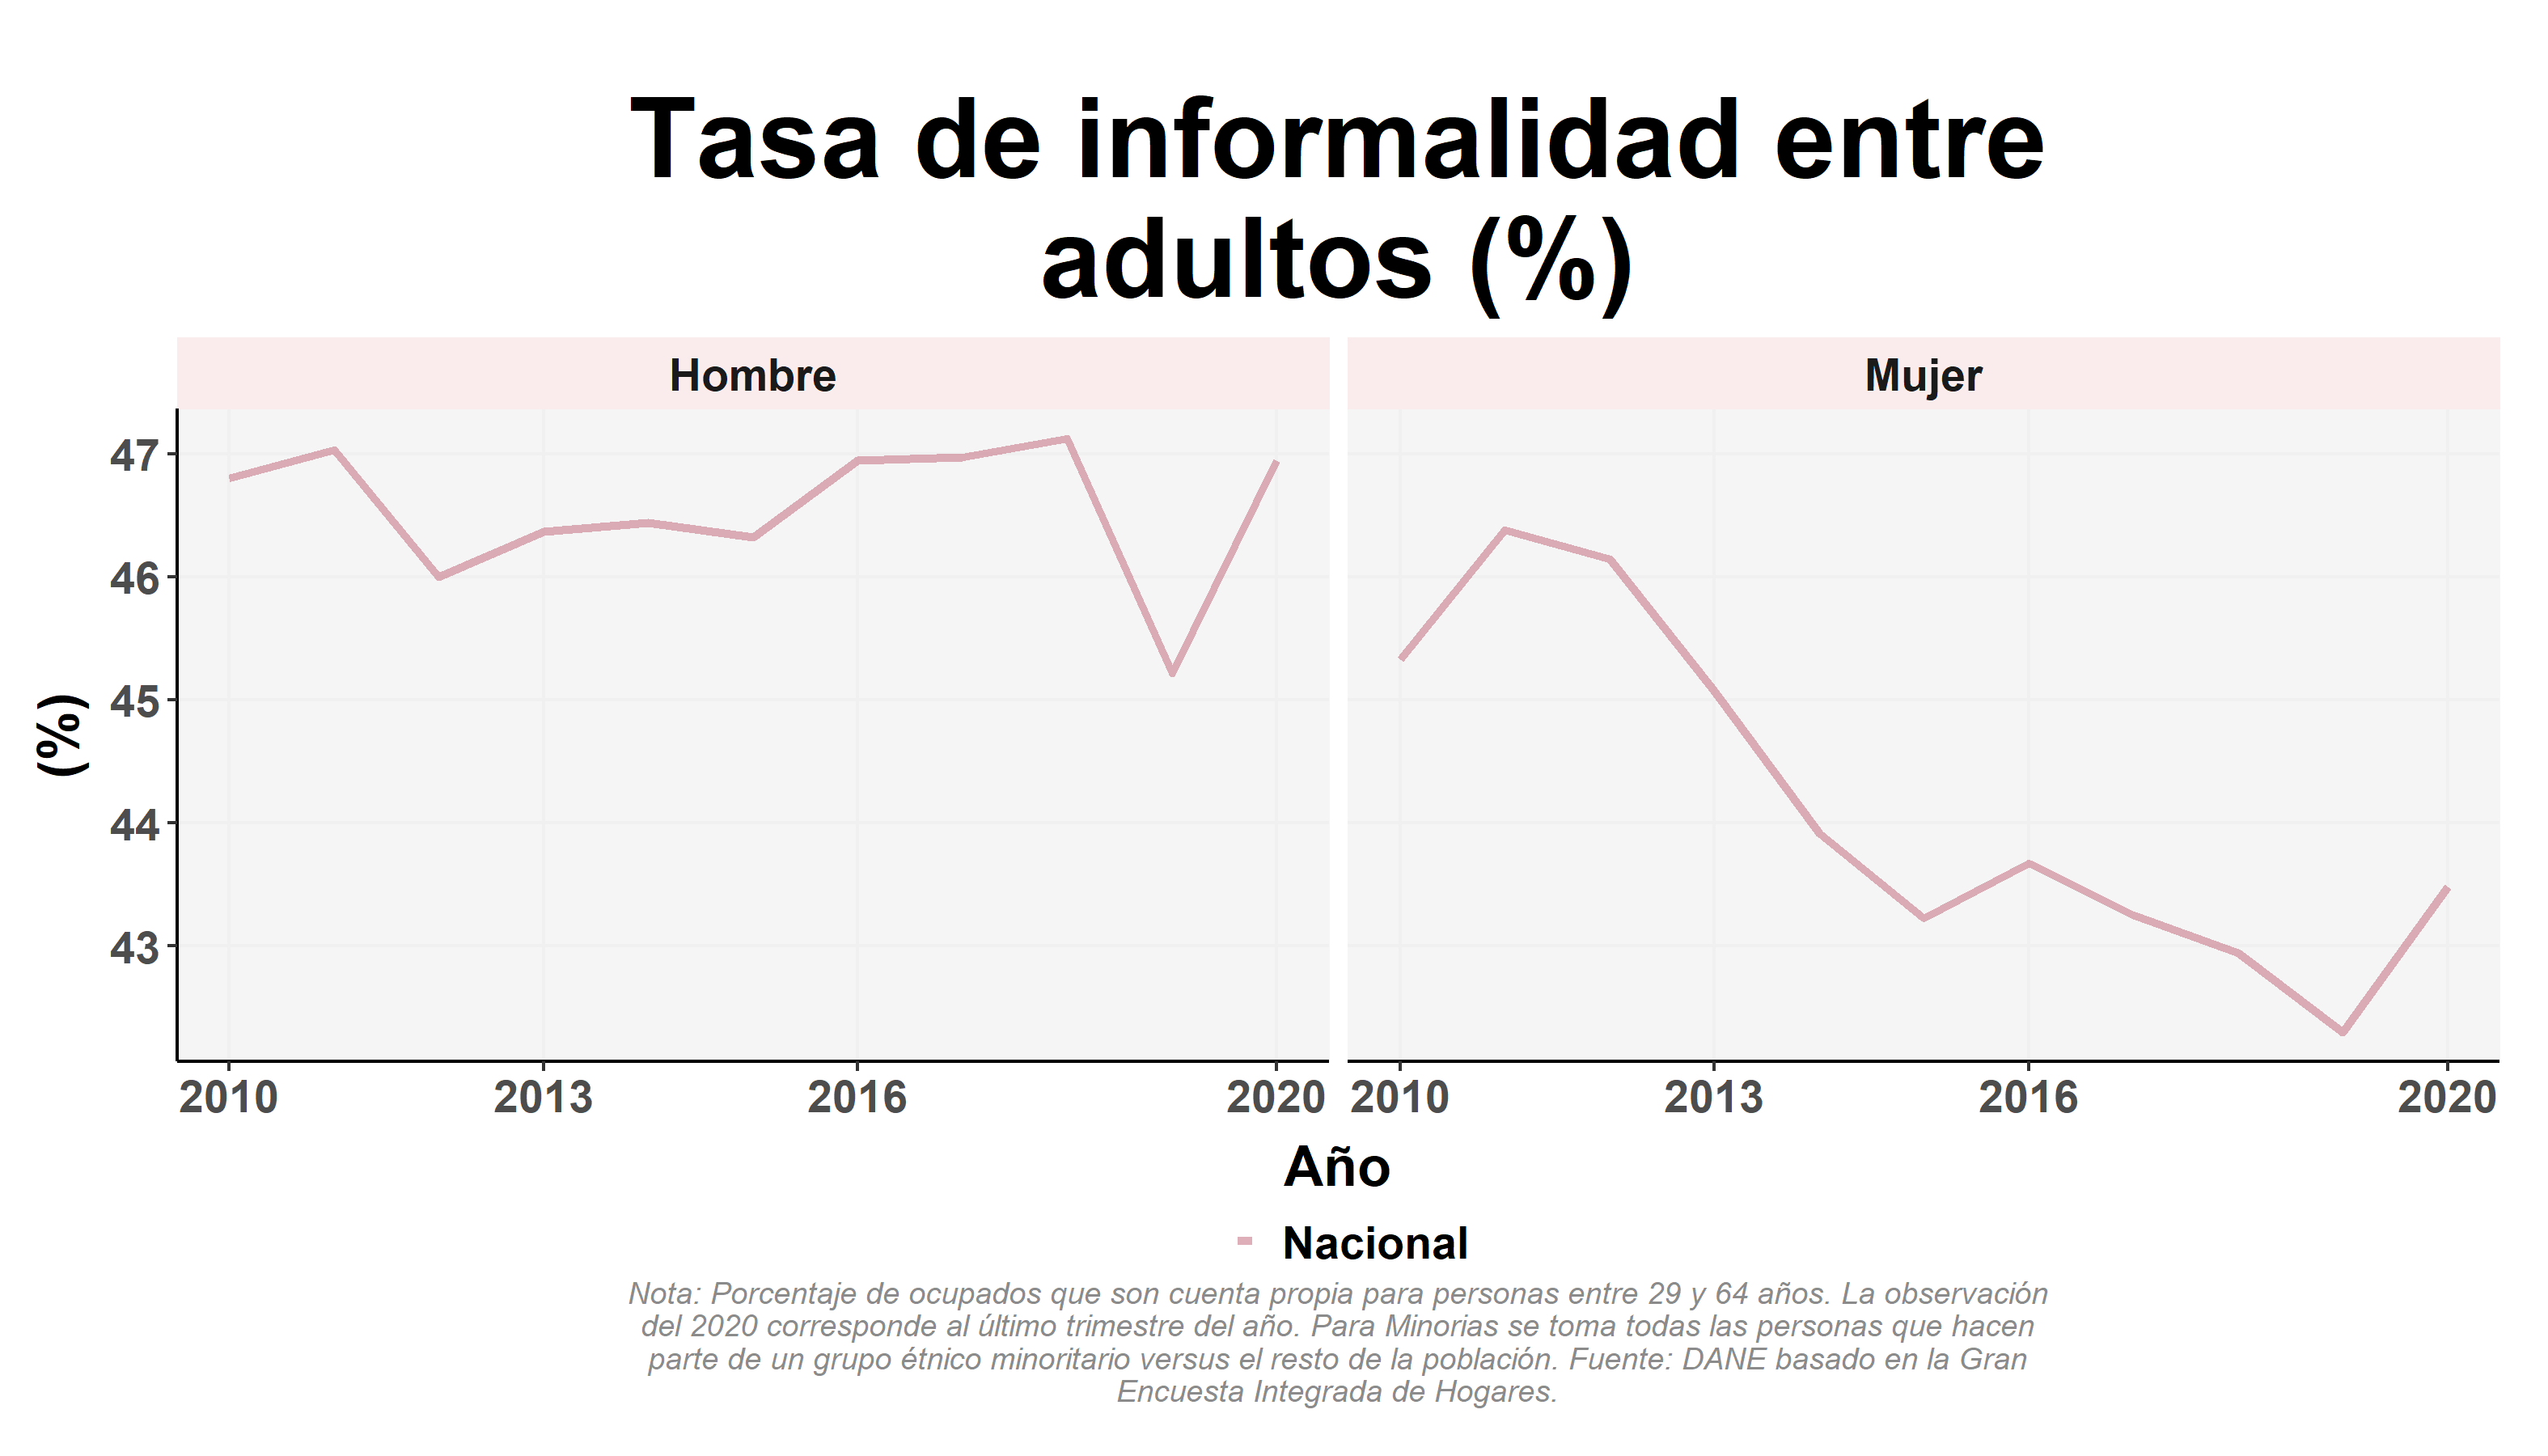
\includegraphics[width=\columnwidth]{img/var_72_trend.png}
            \end{imagecolumn}
            \begin{textcolumn}
                \begin{itemize}
                    \item La informalidad en el país ha disminuido ligeramente en la última década. 
                    \item Especialmente entre las mujeres.
                \end{itemize}
            \end{textcolumn}
    \printcolumns
    \end{slide}    

        %%%-- Homicidios 
        \begin{slide}{15} 
            \begin{imagecolumn}
                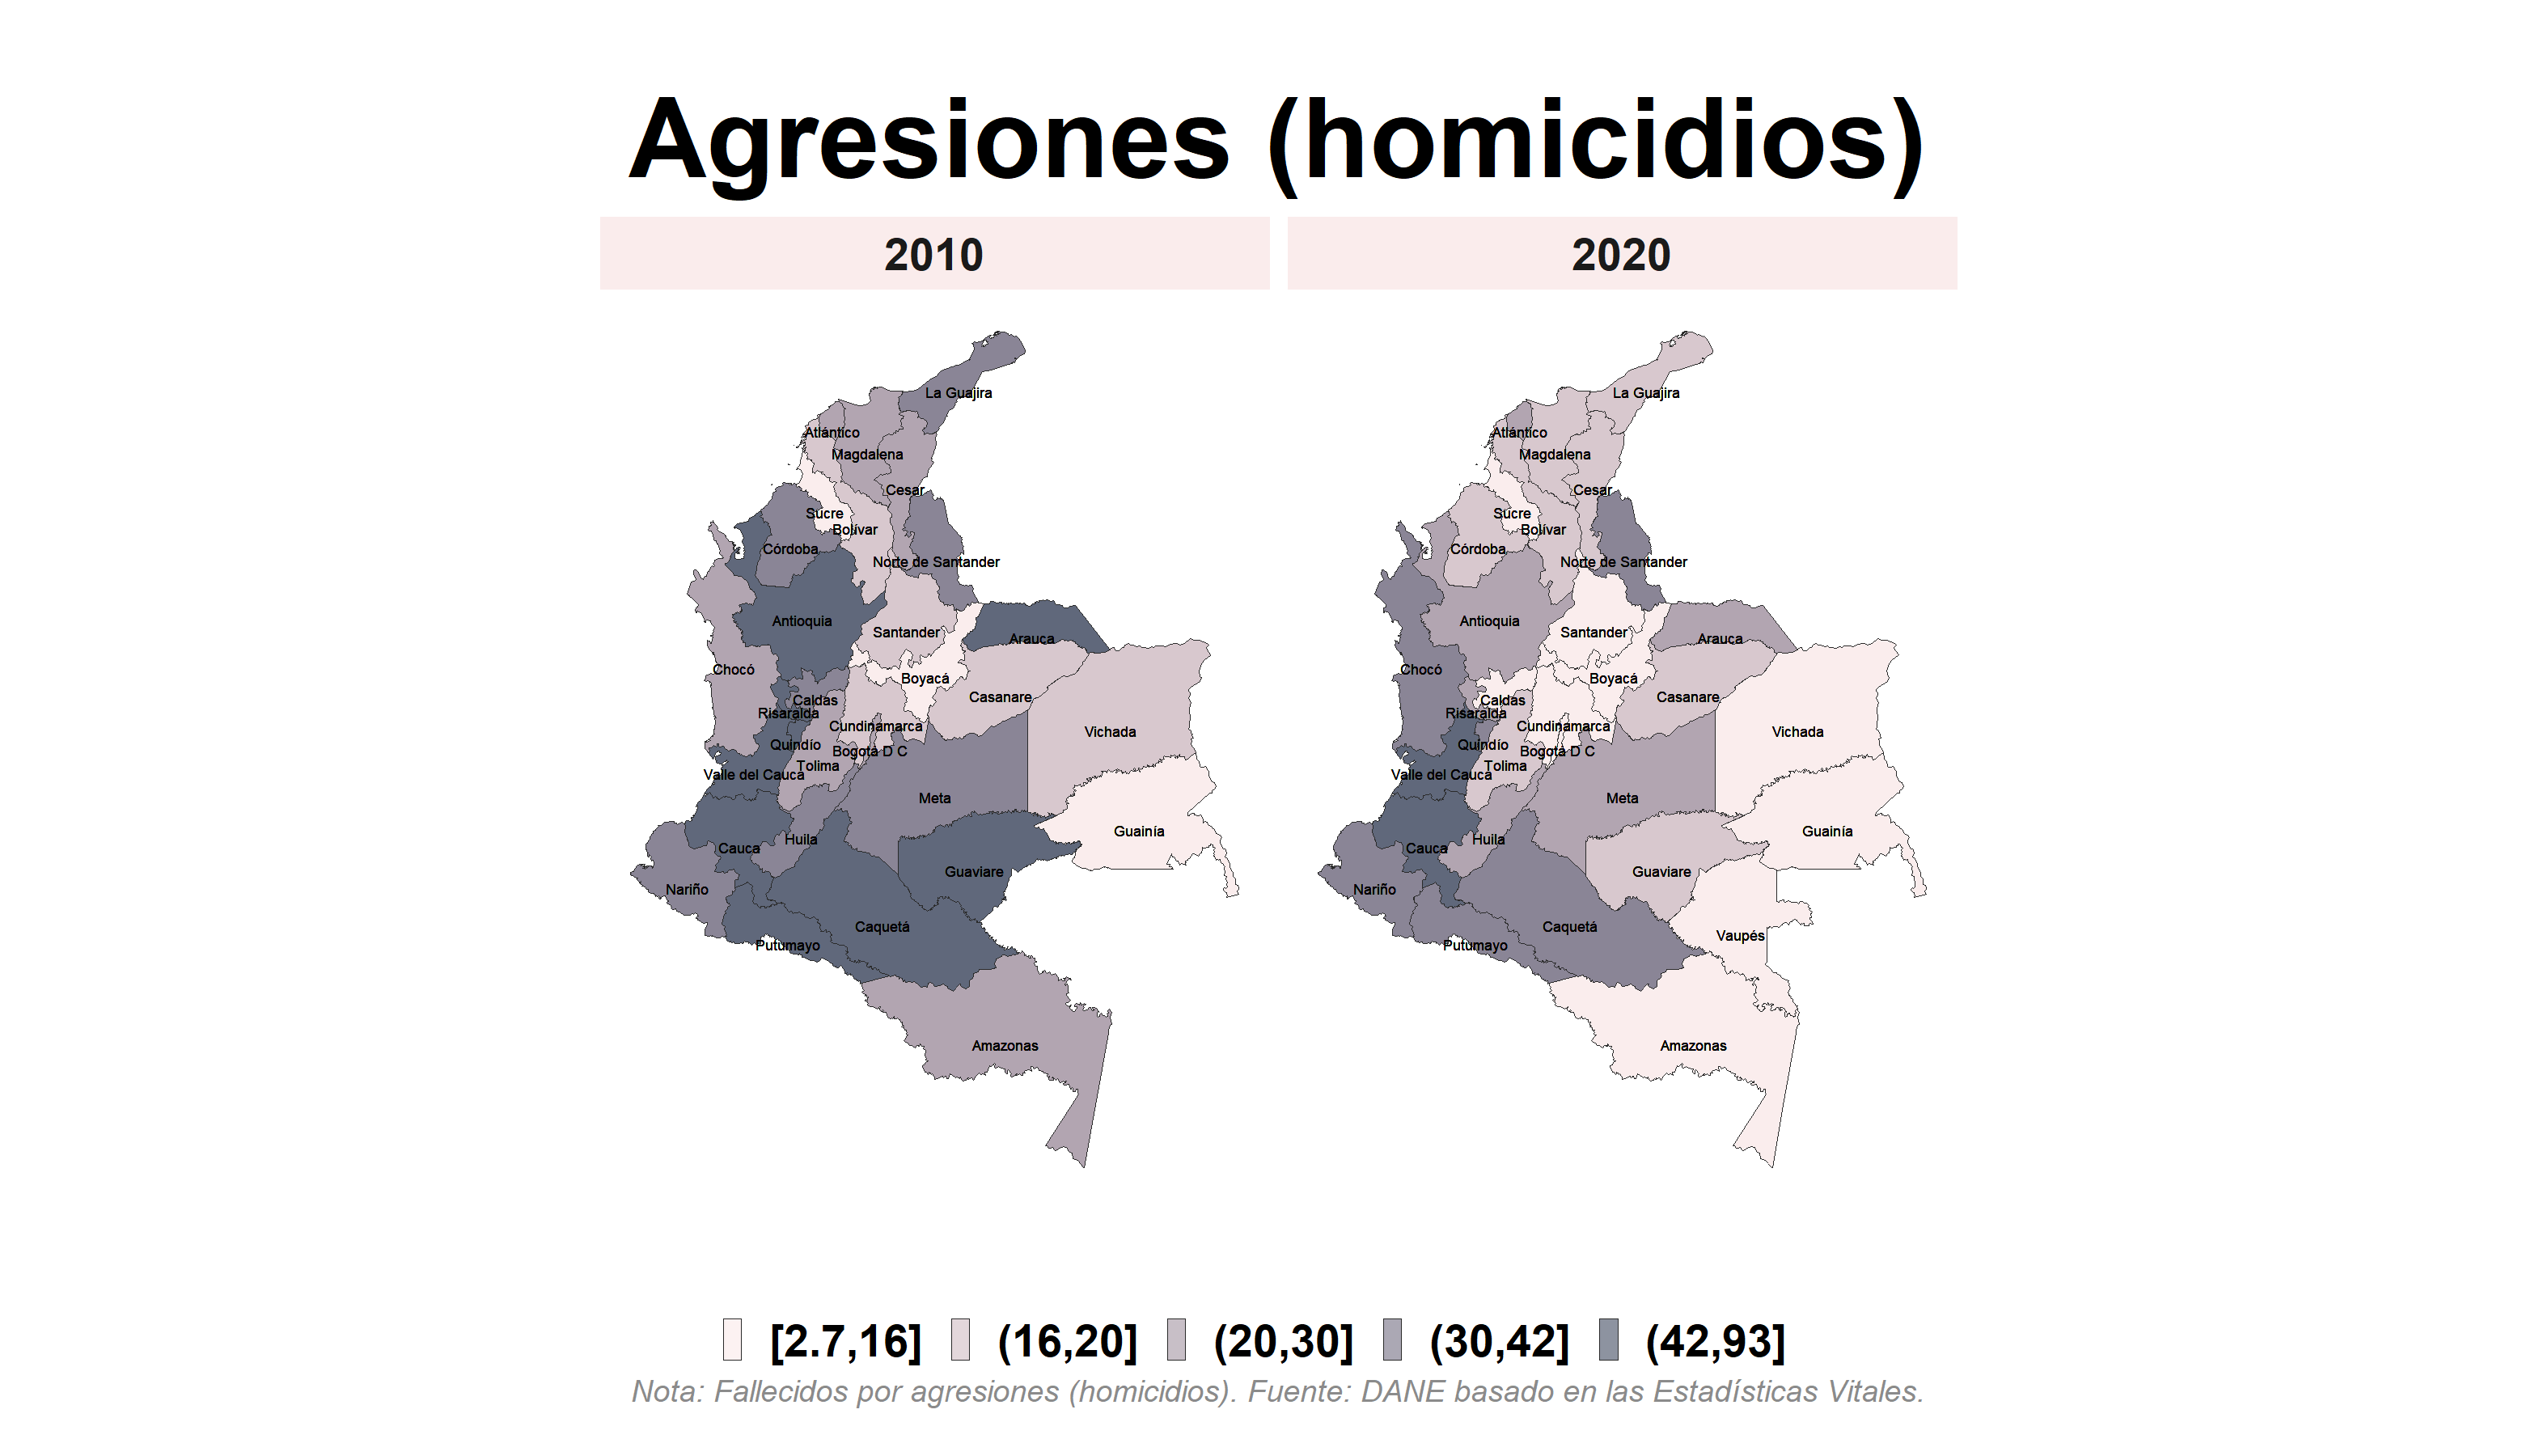
\includegraphics[width=\columnwidth]{img/var_286_map.png}
            \end{imagecolumn}
            \begin{textcolumn}
                \begin{itemize}
                    \item Una tendencia a la baja en los homicidios, pero con una alta concentración territorial.
                \end{itemize}
            \end{textcolumn}
    \printcolumns
    \end{slide}
    
        %%%-- salud mental 
        \begin{slide}{15} 
            \begin{imagecolumn}
                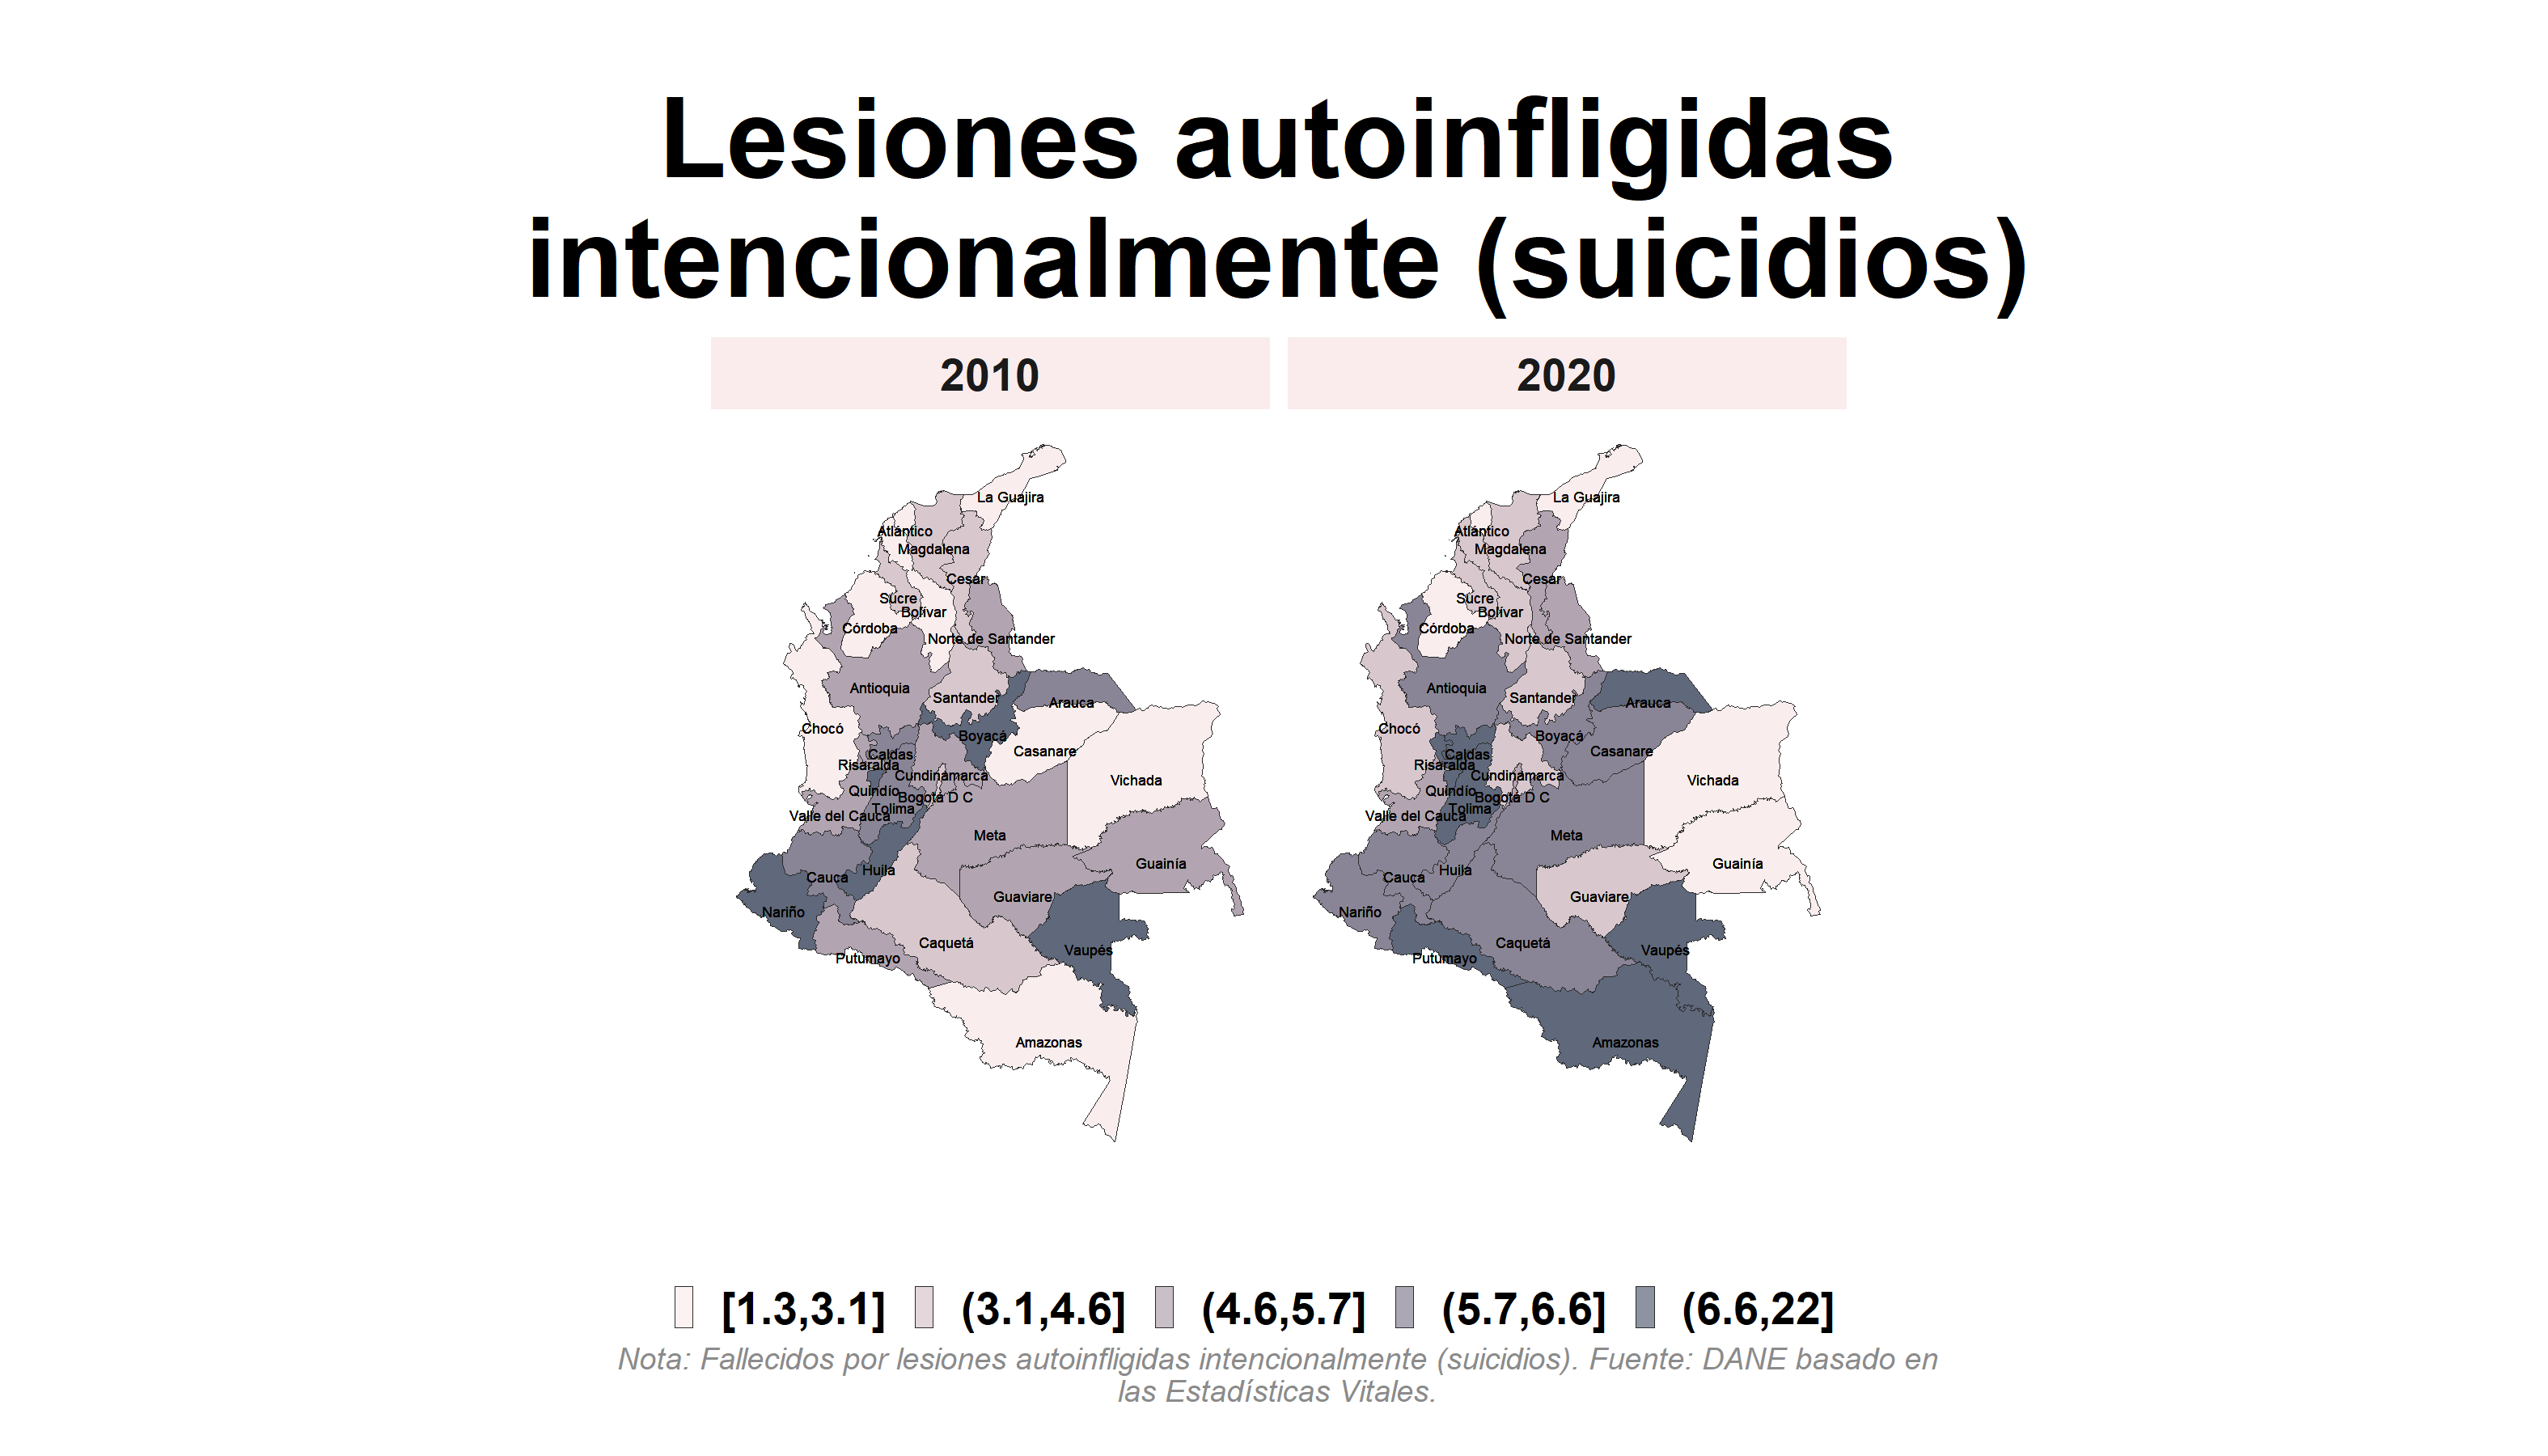
\includegraphics[width=\columnwidth]{img/var_294_map.png}
            \end{imagecolumn}
            \begin{textcolumn}
                \begin{itemize}
                    \item La salud mental ha empeorado a nivel nacional
                    \item La tasa de suicidios es particularmente alta en algunas zonas del centro del país.
                \end{itemize}
            \end{textcolumn}
    \printcolumns
    \end{slide}
    
          %%% ----------------------------
    %%% Machine Learning
    %%% ----------------------------
      \section{Colombias}
    %%% Contexto
    \slidetitle{17}
    
                %%%-- Highlights 
    \begin{slide}{18} 
            \begin{imagecolumn}
                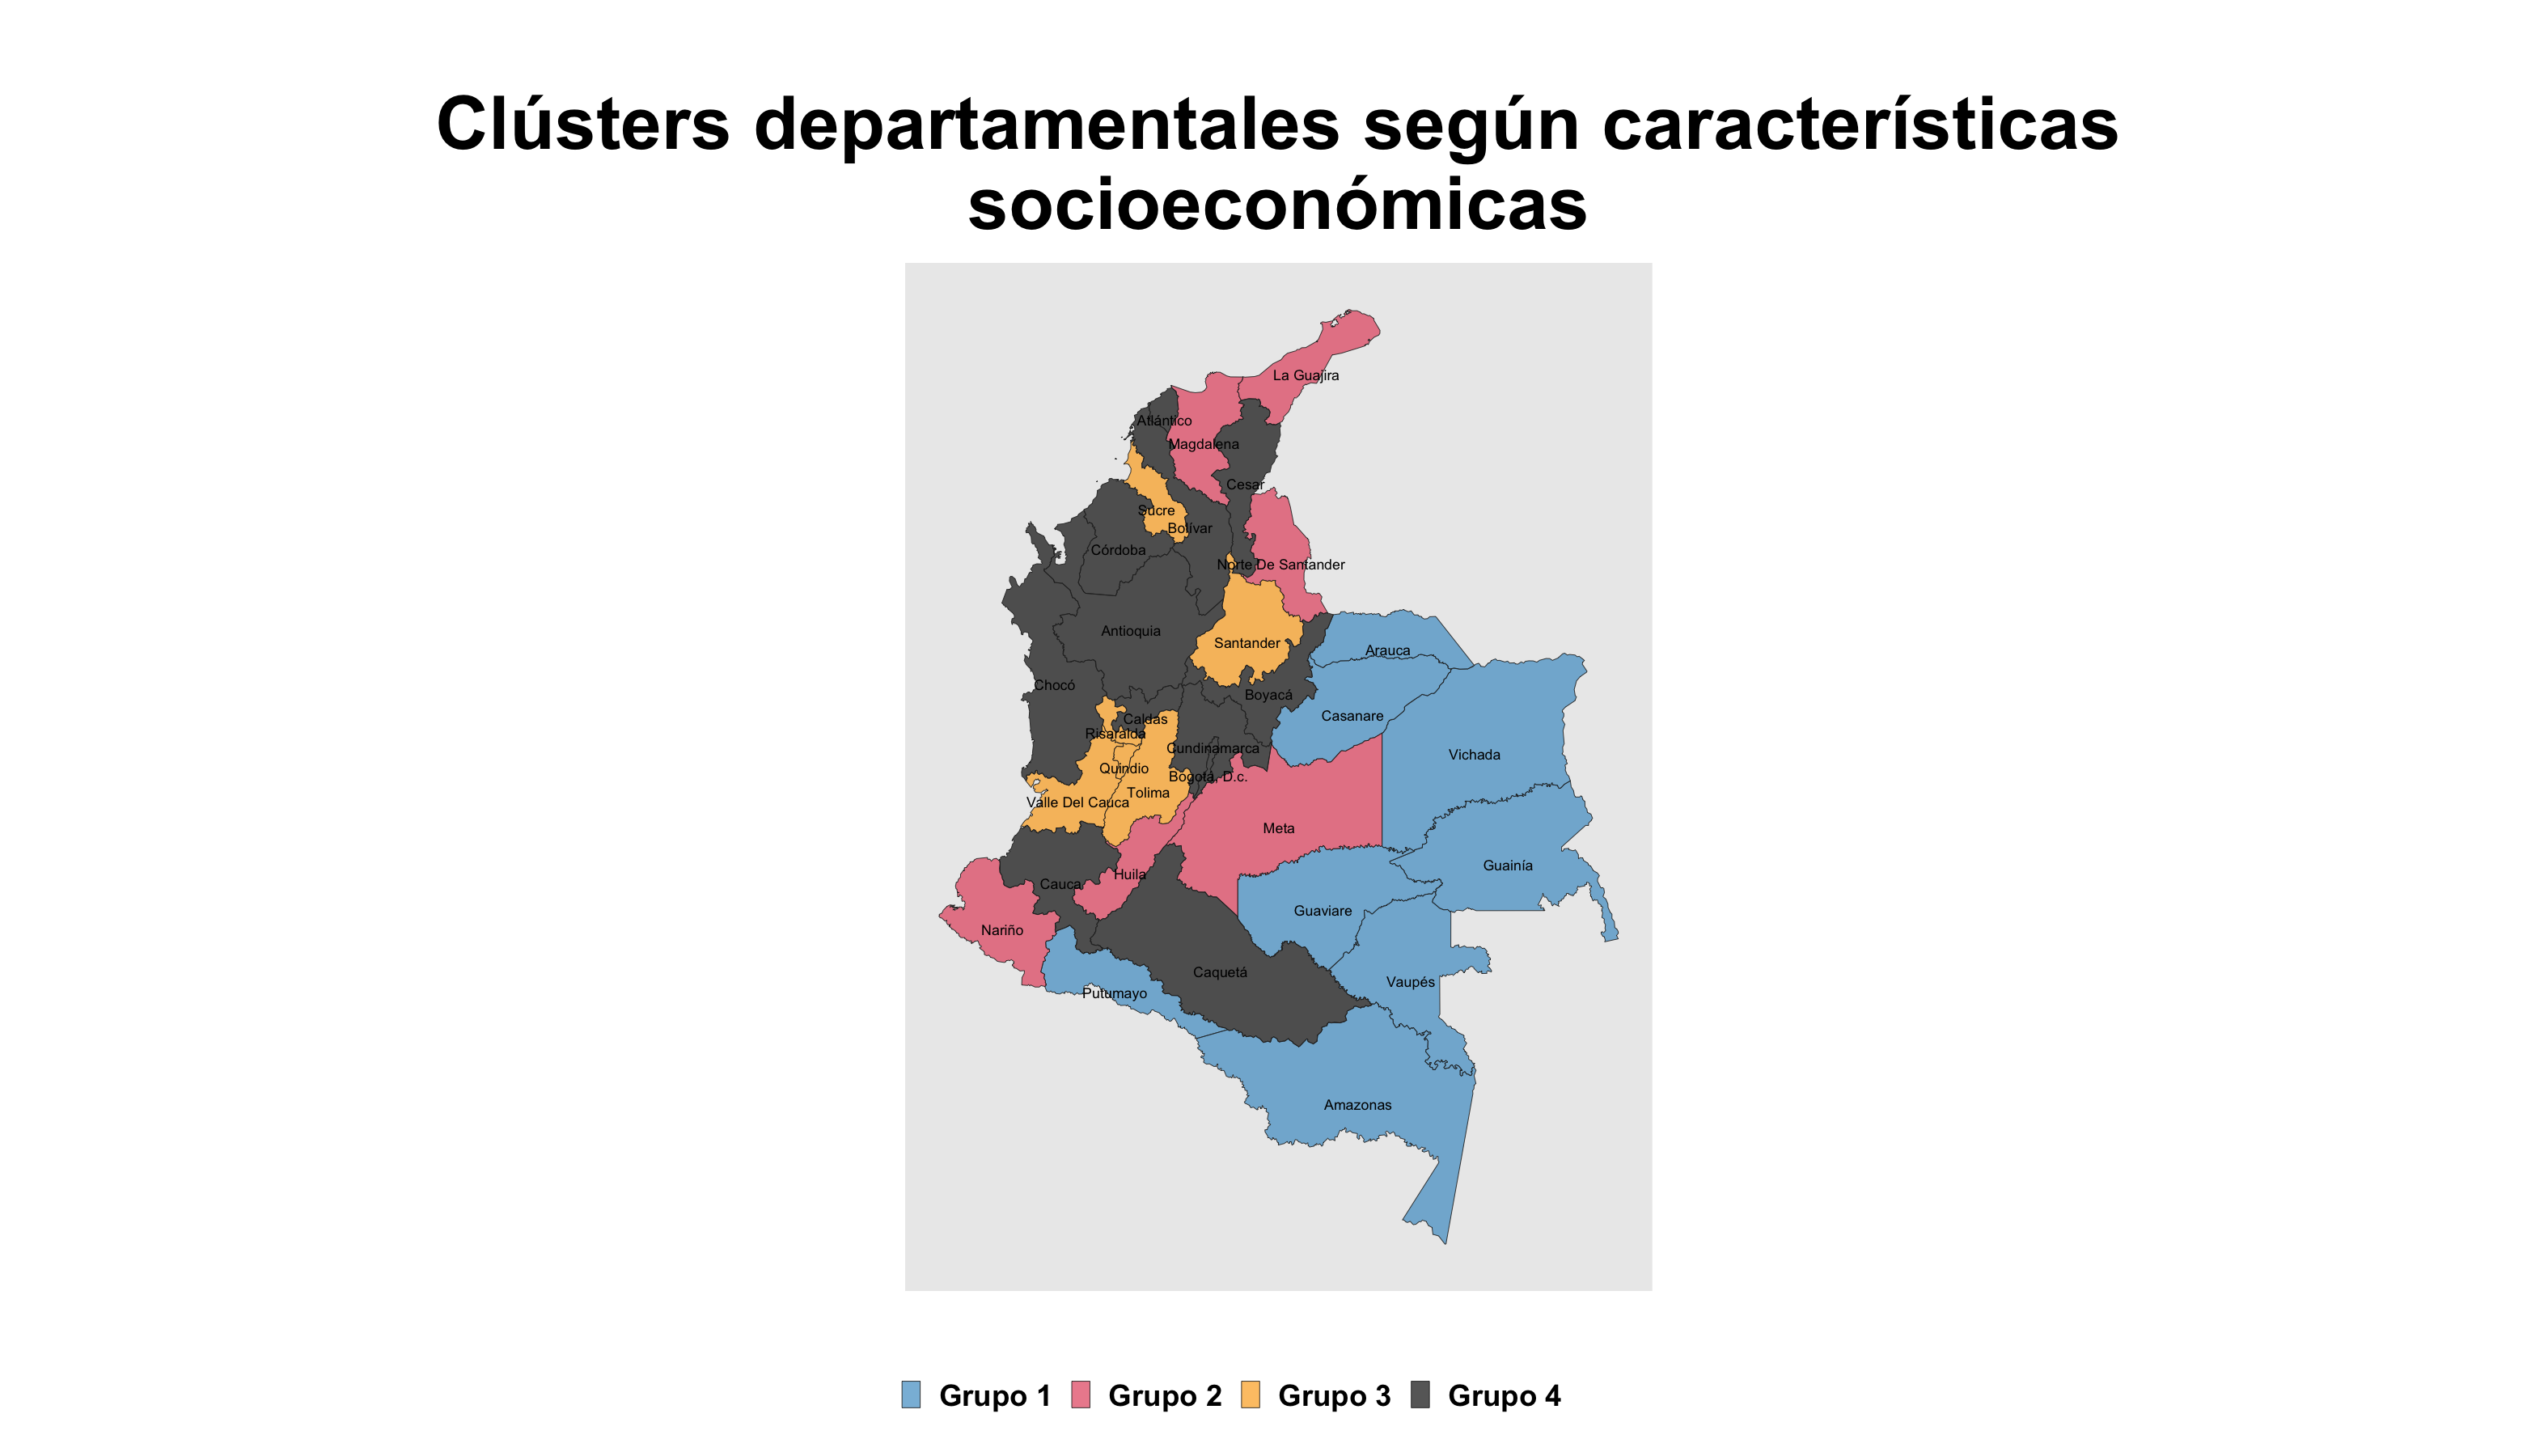
\includegraphics[width=\columnwidth]{img/cluster_main.png}
            \end{imagecolumn}
            \begin{textcolumn}
                \begin{itemize}
                    \item Índice por cada dimensión
                    \item 4 grupos de departamentos
                \end{itemize}
            \end{textcolumn}
    \printcolumns
    \end{slide}
    
        %%% Contexto
    \slidetitle{19}
    
    
   
\end{document}